%**************************************%
%*    Generated from PreTeXt source   *%
%*    on 2020-03-12T12:42:58-04:00    *%
%*                                    *%
%*      https://pretextbook.org       *%
%*                                    *%
%**************************************%
\documentclass[oneside,10pt,]{book}
%% Custom Preamble Entries, early (use latex.preamble.early)
%% Default LaTeX packages
%%   1.  always employed (or nearly so) for some purpose, or
%%   2.  a stylewriter may assume their presence
\usepackage{geometry}
%% Some aspects of the preamble are conditional,
%% the LaTeX engine is one such determinant
\usepackage{ifthen}
%% etoolbox has a variety of modern conveniences
\usepackage{etoolbox}
\usepackage{ifxetex,ifluatex}
%% Raster graphics inclusion
\usepackage{graphicx}
%% Color support, xcolor package
%% Always loaded, for: add/delete text, author tools
%% Here, since tcolorbox loads tikz, and tikz loads xcolor
\PassOptionsToPackage{usenames,dvipsnames,svgnames,table}{xcolor}
\usepackage{xcolor}
%% Colored boxes, and much more, though mostly styling
%% skins library provides "enhanced" skin, employing tikzpicture
%% boxes may be configured as "breakable" or "unbreakable"
%% "raster" controls grids of boxes, aka side-by-side
\usepackage{tcolorbox}
\tcbuselibrary{skins}
\tcbuselibrary{breakable}
\tcbuselibrary{raster}
%% We load some "stock" tcolorbox styles that we use a lot
%% Placement here is provisional, there will be some color work also
%% First, black on white, no border, transparent, but no assumption about titles
\tcbset{ bwminimalstyle/.style={size=minimal, boxrule=-0.3pt, frame empty,
colback=white, colbacktitle=white, coltitle=black, opacityfill=0.0} }
%% Second, bold title, run-in to text/paragraph/heading
%% Space afterwards will be controlled by environment,
%% dependent of constructions of the tcb title
\tcbset{ runintitlestyle/.style={fonttitle=\normalfont\bfseries, attach title to upper} }
%% Spacing prior to each exercise, anywhere
\tcbset{ exercisespacingstyle/.style={before skip={1.5ex plus 0.5ex}} }
%% Spacing prior to each block
\tcbset{ blockspacingstyle/.style={before skip={2.0ex plus 0.5ex}} }
%% xparse allows the construction of more robust commands,
%% this is a necessity for isolating styling and behavior
%% The tcolorbox library of the same name loads the base library
\tcbuselibrary{xparse}
%% Hyperref should be here, but likes to be loaded late
%%
%% Inline math delimiters, \(, \), need to be robust
%% 2016-01-31:  latexrelease.sty  supersedes  fixltx2e.sty
%% If  latexrelease.sty  exists, bugfix is in kernel
%% If not, bugfix is in  fixltx2e.sty
%% See:  https://tug.org/TUGboat/tb36-3/tb114ltnews22.pdf
%% and read "Fewer fragile commands" in distribution's  latexchanges.pdf
\IfFileExists{latexrelease.sty}{}{\usepackage{fixltx2e}}
%% Text height identically 9 inches, text width varies on point size
%% See Bringhurst 2.1.1 on measure for recommendations
%% 75 characters per line (count spaces, punctuation) is target
%% which is the upper limit of Bringhurst's recommendations
\geometry{letterpaper,total={340pt,9.0in}}
%% Custom Page Layout Adjustments (use latex.geometry)
%% This LaTeX file may be compiled with pdflatex, xelatex, or lualatex executables
%% LuaTeX is not explicitly supported, but we do accept additions from knowledgeable users
%% The conditional below provides  pdflatex  specific configuration last
%% The following provides engine-specific capabilities
%% Generally, xelatex is necessary non-Western fonts
\ifthenelse{\boolean{xetex} \or \boolean{luatex}}{%
%% begin: xelatex and lualatex-specific configuration
\ifxetex\usepackage{xltxtra}\fi
%% realscripts is the only part of xltxtra relevant to lualatex 
\ifluatex\usepackage{realscripts}\fi
%% fontspec package provides extensive control of system fonts,
%% meaning *.otf (OpenType), and apparently *.ttf (TrueType)
%% that live *outside* your TeX/MF tree, and are controlled by your *system*
%% fontspec will make Latin Modern (lmodern) the default font
\usepackage{fontspec}
%% 
%% Extensive support for other languages
\usepackage{polyglossia}
%% Set main/default language based on pretext/@xml:lang value
%% document language code is "en-US", US English
%% usmax variant has extra hypenation
\setmainlanguage[variant=usmax]{english}
%% Enable secondary languages based on discovery of @xml:lang values
%% Enable fonts/scripts based on discovery of @xml:lang values
%% Western languages should be ably covered by Latin Modern Roman
%% end: xelatex and lualatex-specific configuration
}{%
%% begin: pdflatex-specific configuration
\usepackage[utf8]{inputenc}
%% PreTeXt will create a UTF-8 encoded file
%% begin: font setup and configuration for use with pdflatex
\usepackage{lmodern}
\usepackage[T1]{fontenc}
%% end: font setup and configuration for use with pdflatex
%% end: pdflatex-specific configuration
}
%% Monospace font: Inconsolata (zi4)
%% Sponsored by TUG: http://levien.com/type/myfonts/inconsolata.html
%% Loaded for documents with intentional objects requiring monospace
%% See package documentation for excellent instructions
%% One caveat, seem to need full file name to locate OTF files
%% Loads the "upquote" package as needed, so we don't have to
%% Upright quotes might come from the  textcomp  package, which we also use
%% We employ the shapely \ell to match Google Font version
%% pdflatex: "varqu" option produces best upright quotes
%% xelatex,lualatex: add StylisticSet 1 for shapely \ell
%% xelatex,lualatex: add StylisticSet 2 for plain zero
%% xelatex,lualatex: we add StylisticSet 3 for upright quotes
%% 
\ifthenelse{\boolean{xetex} \or \boolean{luatex}}{%
%% begin: xelatex and lualatex-specific monospace font
\usepackage{zi4}
\setmonofont[BoldFont=Inconsolatazi4-Bold.otf,StylisticSet={1,3}]{Inconsolatazi4-Regular.otf}
%% end: xelatex and lualatex-specific monospace font
}{%
%% begin: pdflatex-specific monospace font
%% "varqu" option provides textcomp \textquotedbl glyph
%% "varl"  option provides shapely "ell"
\usepackage[varqu,varl]{zi4}
%% end: pdflatex-specific monospace font
}
%% Symbols, align environment, bracket-matrix
\usepackage{amsmath}
\usepackage{amssymb}
%% allow page breaks within display mathematics anywhere
%% level 4 is maximally permissive
%% this is exactly the opposite of AMSmath package philosophy
%% there are per-display, and per-equation options to control this
%% split, aligned, gathered, and alignedat are not affected
\allowdisplaybreaks[4]
%% allow more columns to a matrix
%% can make this even bigger by overriding with  latex.preamble.late  processing option
\setcounter{MaxMatrixCols}{30}
%%
%%
%% Division Titles, and Page Headers/Footers
%% titlesec package, loading "titleps" package cooperatively
%% See code comments about the necessity and purpose of "explicit" option
\usepackage[explicit, pagestyles]{titlesec}
\newtitlemark{\chaptertitlename}
%% Set global/default page style for document due
%% to potential re-definitions after documentclass
\pagestyle{headings}
%%
%% Create globally-available macros to be provided for style writers
%% These are redefined for each occurence of each division
\newcommand{\divisionnameptx}{\relax}%
\newcommand{\titleptx}{\relax}%
\newcommand{\subtitleptx}{\relax}%
\newcommand{\shortitleptx}{\relax}%
\newcommand{\authorsptx}{\relax}%
\newcommand{\epigraphptx}{\relax}%
%% Create environments for possible occurences of each division
%% Environment for a PTX "chapter" at the level of a LaTeX "chapter"
\NewDocumentEnvironment{chapterptx}{mmmmmm}
{%
\renewcommand{\divisionnameptx}{Chapter}%
\renewcommand{\titleptx}{#1}%
\renewcommand{\subtitleptx}{#2}%
\renewcommand{\shortitleptx}{#3}%
\renewcommand{\authorsptx}{#4}%
\renewcommand{\epigraphptx}{#5}%
\chapter[{#3}]{#1}%
\label{#6}%
}{}%
%% Environment for a PTX "section" at the level of a LaTeX "section"
\NewDocumentEnvironment{sectionptx}{mmmmmm}
{%
\renewcommand{\divisionnameptx}{Section}%
\renewcommand{\titleptx}{#1}%
\renewcommand{\subtitleptx}{#2}%
\renewcommand{\shortitleptx}{#3}%
\renewcommand{\authorsptx}{#4}%
\renewcommand{\epigraphptx}{#5}%
\section[{#3}]{#1}%
\label{#6}%
}{}%
%% Environment for a PTX "subsection" at the level of a LaTeX "subsection"
\NewDocumentEnvironment{subsectionptx}{mmmmmm}
{%
\renewcommand{\divisionnameptx}{Subsection}%
\renewcommand{\titleptx}{#1}%
\renewcommand{\subtitleptx}{#2}%
\renewcommand{\shortitleptx}{#3}%
\renewcommand{\authorsptx}{#4}%
\renewcommand{\epigraphptx}{#5}%
\subsection[{#3}]{#1}%
\label{#6}%
}{}%
%% Environment for a PTX "subsubsection" at the level of a LaTeX "subsubsection"
\NewDocumentEnvironment{subsubsectionptx}{mmmmmm}
{%
\renewcommand{\divisionnameptx}{Subsubsection}%
\renewcommand{\titleptx}{#1}%
\renewcommand{\subtitleptx}{#2}%
\renewcommand{\shortitleptx}{#3}%
\renewcommand{\authorsptx}{#4}%
\renewcommand{\epigraphptx}{#5}%
\subsubsection[{#3}]{#1}%
\label{#6}%
}{}%
%% Environment for a PTX "appendix" at the level of a LaTeX "chapter"
\NewDocumentEnvironment{appendixptx}{mmmmmm}
{%
\renewcommand{\divisionnameptx}{Appendix}%
\renewcommand{\titleptx}{#1}%
\renewcommand{\subtitleptx}{#2}%
\renewcommand{\shortitleptx}{#3}%
\renewcommand{\authorsptx}{#4}%
\renewcommand{\epigraphptx}{#5}%
\chapter[{#3}]{#1}%
\label{#6}%
}{}%
%% Environment for a PTX "exercises" at the level of a LaTeX "subsection"
\NewDocumentEnvironment{exercises-subsection}{mmmmmm}
{%
\renewcommand{\divisionnameptx}{Exercises}%
\renewcommand{\titleptx}{#1}%
\renewcommand{\subtitleptx}{#2}%
\renewcommand{\shortitleptx}{#3}%
\renewcommand{\authorsptx}{#4}%
\renewcommand{\epigraphptx}{#5}%
\subsection[{#3}]{#1}%
\label{#6}%
}{}%
%% Environment for a PTX "exercises" at the level of a LaTeX "subsection"
\NewDocumentEnvironment{exercises-subsection-numberless}{mmmmmm}
{%
\renewcommand{\divisionnameptx}{Exercises}%
\renewcommand{\titleptx}{#1}%
\renewcommand{\subtitleptx}{#2}%
\renewcommand{\shortitleptx}{#3}%
\renewcommand{\authorsptx}{#4}%
\renewcommand{\epigraphptx}{#5}%
\subsection*{#1}%
\addcontentsline{toc}{subsection}{#3}
\label{#6}%
}{}%
%% Environment for a PTX "exercises" at the level of a LaTeX "subsubsection"
\NewDocumentEnvironment{exercises-subsubsection}{mmmmmm}
{%
\renewcommand{\divisionnameptx}{Exercises}%
\renewcommand{\titleptx}{#1}%
\renewcommand{\subtitleptx}{#2}%
\renewcommand{\shortitleptx}{#3}%
\renewcommand{\authorsptx}{#4}%
\renewcommand{\epigraphptx}{#5}%
\subsubsection[{#3}]{#1}%
\label{#6}%
}{}%
%% Environment for a PTX "exercises" at the level of a LaTeX "subsubsection"
\NewDocumentEnvironment{exercises-subsubsection-numberless}{mmmmmm}
{%
\renewcommand{\divisionnameptx}{Exercises}%
\renewcommand{\titleptx}{#1}%
\renewcommand{\subtitleptx}{#2}%
\renewcommand{\shortitleptx}{#3}%
\renewcommand{\authorsptx}{#4}%
\renewcommand{\epigraphptx}{#5}%
\subsubsection*{#1}%
\addcontentsline{toc}{subsubsection}{#3}
\label{#6}%
}{}%
%%
%% Styles for six traditional LaTeX divisions
\titleformat{\chapter}[display]
{\normalfont\huge\bfseries}{\divisionnameptx\space\thechapter}{20pt}{\Huge#1}
[{\Large\authorsptx}]
\titleformat{name=\chapter,numberless}[display]
{\normalfont\huge\bfseries}{}{0pt}{#1}
[{\Large\authorsptx}]
\titlespacing*{\chapter}{0pt}{50pt}{40pt}
\titleformat{\section}[hang]
{\normalfont\Large\bfseries}{\thesection}{1ex}{#1}
[{\large\authorsptx}]
\titleformat{name=\section,numberless}[block]
{\normalfont\Large\bfseries}{}{0pt}{#1}
[{\large\authorsptx}]
\titlespacing*{\section}{0pt}{3.5ex plus 1ex minus .2ex}{2.3ex plus .2ex}
\titleformat{\subsection}[hang]
{\normalfont\large\bfseries}{\thesubsection}{1ex}{#1}
[{\normalsize\authorsptx}]
\titleformat{name=\subsection,numberless}[block]
{\normalfont\large\bfseries}{}{0pt}{#1}
[{\normalsize\authorsptx}]
\titlespacing*{\subsection}{0pt}{3.25ex plus 1ex minus .2ex}{1.5ex plus .2ex}
\titleformat{\subsubsection}[hang]
{\normalfont\normalsize\bfseries}{\thesubsubsection}{1em}{#1}
[{\small\authorsptx}]
\titleformat{name=\subsubsection,numberless}[block]
{\normalfont\normalsize\bfseries}{}{0pt}{#1}
[{\normalsize\authorsptx}]
\titlespacing*{\subsubsection}{0pt}{3.25ex plus 1ex minus .2ex}{1.5ex plus .2ex}
\titleformat{\paragraph}[hang]
{\normalfont\normalsize\bfseries}{\theparagraph}{1em}{#1}
[{\small\authorsptx}]
\titleformat{name=\paragraph,numberless}[block]
{\normalfont\normalsize\bfseries}{}{0pt}{#1}
[{\normalsize\authorsptx}]
\titlespacing*{\paragraph}{0pt}{3.25ex plus 1ex minus .2ex}{1.5em}
%%
%% Semantic Macros
%% To preserve meaning in a LaTeX file
%%
%% \mono macro for content of "c", "cd", "tag", etc elements
%% Also used automatically in other constructions
%% Simply an alias for \texttt
%% Always defined, even if there is no need, or if a specific tt font is not loaded
\newcommand{\mono}[1]{\texttt{#1}}
%%
%% Following semantic macros are only defined here if their
%% use is required only in this specific document
%%
%% Used for warnings, typically bold and italic
\newcommand{\alert}[1]{\textbf{\textit{#1}}}
%% Used for inline definitions of terms
\newcommand{\terminology}[1]{\textbf{#1}}
%% Division Numbering: Chapters, Sections, Subsections, etc
%% Division numbers may be turned off at some level ("depth")
%% A section *always* has depth 1, contrary to us counting from the document root
%% The latex default is 3.  If a larger number is present here, then
%% removing this command may make some cross-references ambiguous
%% The precursor variable $numbering-maxlevel is checked for consistency in the common XSL file
\setcounter{secnumdepth}{3}
%%
%% AMS "proof" environment is no longer used, but we leave previously
%% implemented \qedhere in place, should the LaTeX be recycled
\newcommand{\qedhere}{\relax}
%%
%% A faux tcolorbox whose only purpose is to provide common numbering
%% facilities for most blocks (possibly not projects, 2D displays)
%% Controlled by  numbering.theorems.level  processing parameter
\newtcolorbox[auto counter, number within=section]{block}{}
%%
%% This document is set to number PROJECT-LIKE on a separate numbering scheme
%% So, a faux tcolorbox whose only purpose is to provide this numbering
%% Controlled by  numbering.projects.level  processing parameter
\newtcolorbox[auto counter, number within=section]{project-distinct}{}
%% A faux tcolorbox whose only purpose is to provide common numbering
%% facilities for 2D displays which are subnumbered as part of a "sidebyside"
\newtcolorbox[auto counter, number within=tcb@cnt@block, number freestyle={\noexpand\thetcb@cnt@block(\noexpand\alph{\tcbcounter})}]{subdisplay}{}
%%
%% tcolorbox, with styles, for THEOREM-LIKE
%%
%% theorem: fairly simple numbered block/structure
\tcbset{ theoremstyle/.style={bwminimalstyle, runintitlestyle, blockspacingstyle, after title={\space}, } }
\newtcolorbox[use counter from=block]{theorem}[3]{title={{Theorem~\thetcbcounter\notblank{#1#2}{\space}{}\notblank{#1}{\space#1}{}\notblank{#2}{\space(#2)}{}}}, phantomlabel={#3}, breakable, parbox=false, after={\par}, fontupper=\itshape, theoremstyle, }
%% corollary: fairly simple numbered block/structure
\tcbset{ corollarystyle/.style={bwminimalstyle, runintitlestyle, blockspacingstyle, after title={\space}, } }
\newtcolorbox[use counter from=block]{corollary}[3]{title={{Corollary~\thetcbcounter\notblank{#1#2}{\space}{}\notblank{#1}{\space#1}{}\notblank{#2}{\space(#2)}{}}}, phantomlabel={#3}, breakable, parbox=false, after={\par}, fontupper=\itshape, corollarystyle, }
%%
%% tcolorbox, with styles, for DEFINITION-LIKE
%%
%% definition: fairly simple numbered block/structure
\tcbset{ definitionstyle/.style={bwminimalstyle, runintitlestyle, blockspacingstyle, after title={\space}, after upper={\space\space\hspace*{\stretch{1}}\(\lozenge\)}, } }
\newtcolorbox[use counter from=block]{definition}[2]{title={{Definition~\thetcbcounter\notblank{#1}{\space\space#1}{}}}, phantomlabel={#2}, breakable, parbox=false, after={\par}, definitionstyle, }
%%
%% tcolorbox, with styles, for REMARK-LIKE
%%
%% observation: fairly simple numbered block/structure
\tcbset{ observationstyle/.style={bwminimalstyle, runintitlestyle, blockspacingstyle, after title={\space}, } }
\newtcolorbox[use counter from=block]{observation}[2]{title={{Observation~\thetcbcounter\notblank{#1}{\space\space#1}{}}}, phantomlabel={#2}, breakable, parbox=false, after={\par}, observationstyle, }
%%
%% tcolorbox, with styles, for EXAMPLE-LIKE
%%
%% example: fairly simple numbered block/structure
\tcbset{ examplestyle/.style={bwminimalstyle, runintitlestyle, blockspacingstyle, after title={\space}, after upper={\space\space\hspace*{\stretch{1}}\(\square\)}, } }
\newtcolorbox[use counter from=block]{example}[2]{title={{Example~\thetcbcounter\notblank{#1}{\space\space#1}{}}}, phantomlabel={#2}, breakable, parbox=false, after={\par}, examplestyle, }
%%
%% tcolorbox, with styles, for FIGURE-LIKE
%%
%% figureptx: 2-D display structure
\tcbset{ figureptxstyle/.style={bwminimalstyle, middle=1ex, blockspacingstyle, } }
\newtcolorbox[use counter from=block]{figureptx}[3]{lower separated=false, before lower={{\textbf{Figure~\thetcbcounter}\space#1}}, phantomlabel={#2}, unbreakable, parbox=false, figureptxstyle, }
%%
%% xparse environments for introductions and conclusions of divisions
%%
%% introduction: in a structured division
\NewDocumentEnvironment{introduction}{m}
{\notblank{#1}{\noindent\textbf{#1}\space}{}}{\par\medskip}
%%
%% tcolorbox, with styles, for miscellaneous environments
%%
%% assemblage: fairly simple un-numbered block/structure
\tcbset{ assemblagestyle/.style={size=normal, colback=white, colbacktitle=white, coltitle=black, colframe=black, rounded corners, titlerule=0.0pt, center title, fonttitle=\normalfont\bfseries, blockspacingstyle, } }
\newtcolorbox{assemblage}[2]{title={\notblank{#1}{#1}{}}, phantomlabel={#2}, breakable, parbox=false, assemblagestyle}
%% proof: title is a replacement
\tcbset{ proofstyle/.style={bwminimalstyle, fonttitle=\normalfont\itshape, attach title to upper, after title={\space}, after upper={\space\space\hspace*{\stretch{1}}\(\blacksquare\)},
} }
\newtcolorbox{proofptx}[2]{title={\notblank{#1}{#1}{Proof.}}, phantom={\hypertarget{#2}{}}, breakable, parbox=false, after={\par}, proofstyle }
%% Divisional exercises (and worksheet) as LaTeX environments
%% Third argument is option for extra workspace in worksheets
%% Hanging indent occupies a 5ex width slot prior to left margin
%% Experimentally this seems just barely sufficient for a bold "888."
%% Division exercises, not in exercise group
\tcbset{ divisionexercisestyle/.style={bwminimalstyle, runintitlestyle, exercisespacingstyle, left=5ex, breakable, parbox=false } }
\newtcolorbox{divisionexercise}[4]{divisionexercisestyle, before title={\hspace{-5ex}\makebox[5ex][l]{#1.}}, title={\notblank{#2}{#2\space}{}}, phantom={\hypertarget{#4}{}}, after={\notblank{#3}{\newline\rule{\workspacestrutwidth}{#3\textheight}\newline}{}}}
%% Localize LaTeX supplied names (possibly none)
\renewcommand*{\appendixname}{Appendix}
\renewcommand*{\chaptername}{Chapter}
%% Equation Numbering
%% Controlled by  numbering.equations.level  processing parameter
%% No adjustment here implies document-wide numbering
\numberwithin{equation}{section}
%% "tcolorbox" environment for a single image, occupying entire \linewidth
%% arguments are left-margin, width, right-margin, as multiples of
%% \linewidth, and are guaranteed to be positive and sum to 1.0
\tcbset{ imagestyle/.style={bwminimalstyle} }
\NewTColorBox{image}{mmm}{imagestyle,left skip=#1\linewidth,width=#2\linewidth}
%% For improved tables
\usepackage{array}
%% Some extra height on each row is desirable, especially with horizontal rules
%% Increment determined experimentally
\setlength{\extrarowheight}{0.2ex}
%% Define variable thickness horizontal rules, full and partial
%% Thicknesses are 0.03, 0.05, 0.08 in the  booktabs  package
\newcommand{\hrulethin}  {\noalign{\hrule height 0.04em}}
\newcommand{\hrulemedium}{\noalign{\hrule height 0.07em}}
\newcommand{\hrulethick} {\noalign{\hrule height 0.11em}}
%% We preserve a copy of the \setlength package before other
%% packages (extpfeil) get a chance to load packages that redefine it
\let\oldsetlength\setlength
\newlength{\Oldarrayrulewidth}
\newcommand{\crulethin}[1]%
{\noalign{\global\oldsetlength{\Oldarrayrulewidth}{\arrayrulewidth}}%
\noalign{\global\oldsetlength{\arrayrulewidth}{0.04em}}\cline{#1}%
\noalign{\global\oldsetlength{\arrayrulewidth}{\Oldarrayrulewidth}}}%
\newcommand{\crulemedium}[1]%
{\noalign{\global\oldsetlength{\Oldarrayrulewidth}{\arrayrulewidth}}%
\noalign{\global\oldsetlength{\arrayrulewidth}{0.07em}}\cline{#1}%
\noalign{\global\oldsetlength{\arrayrulewidth}{\Oldarrayrulewidth}}}
\newcommand{\crulethick}[1]%
{\noalign{\global\oldsetlength{\Oldarrayrulewidth}{\arrayrulewidth}}%
\noalign{\global\oldsetlength{\arrayrulewidth}{0.11em}}\cline{#1}%
\noalign{\global\oldsetlength{\arrayrulewidth}{\Oldarrayrulewidth}}}
%% Single letter column specifiers defined via array package
\newcolumntype{A}{!{\vrule width 0.04em}}
\newcolumntype{B}{!{\vrule width 0.07em}}
\newcolumntype{C}{!{\vrule width 0.11em}}
%% Program listing support: for listings, programs, consoles, and Sage code
\ifthenelse{\boolean{xetex} \or \boolean{luatex}}%
  {\tcbuselibrary{listings}}%
  {\tcbuselibrary{listingsutf8}}%
%% We define the listings font style to be the default "ttfamily"
%% To fix hyphens/dashes rendered in PDF as fancy minus signs by listing
%% http://tex.stackexchange.com/questions/33185/listings-package-changes-hyphens-to-minus-signs
\makeatletter
\lst@CCPutMacro\lst@ProcessOther {"2D}{\lst@ttfamily{-{}}{-{}}}
\@empty\z@\@empty
\makeatother
%% We define a null language, free of any formatting or style
%% for use when a language is not supported, or pseudo-code, or consoles
%% Not necessary for Sage code, so in limited cases included unnecessarily
\lstdefinelanguage{none}{identifierstyle=,commentstyle=,stringstyle=,keywordstyle=}
\ifthenelse{\boolean{xetex}}{}{%
%% begin: pdflatex-specific listings configuration
%% translate U+0080 - U+00F0 to their textmode LaTeX equivalents
%% Data originally from https://www.w3.org/Math/characters/unicode.xml, 2016-07-23
%% Lines marked in XSL with "$" were converted from mathmode to textmode
\lstset{extendedchars=true}
\lstset{literate={ }{{~}}{1}{¡}{{\textexclamdown }}{1}{¢}{{\textcent }}{1}{£}{{\textsterling }}{1}{¤}{{\textcurrency }}{1}{¥}{{\textyen }}{1}{¦}{{\textbrokenbar }}{1}{§}{{\textsection }}{1}{¨}{{\textasciidieresis }}{1}{©}{{\textcopyright }}{1}{ª}{{\textordfeminine }}{1}{«}{{\guillemotleft }}{1}{¬}{{\textlnot }}{1}{­}{{\-}}{1}{®}{{\textregistered }}{1}{¯}{{\textasciimacron }}{1}{°}{{\textdegree }}{1}{±}{{\textpm }}{1}{²}{{\texttwosuperior }}{1}{³}{{\textthreesuperior }}{1}{´}{{\textasciiacute }}{1}{µ}{{\textmu }}{1}{¶}{{\textparagraph }}{1}{·}{{\textperiodcentered }}{1}{¸}{{\c{}}}{1}{¹}{{\textonesuperior }}{1}{º}{{\textordmasculine }}{1}{»}{{\guillemotright }}{1}{¼}{{\textonequarter }}{1}{½}{{\textonehalf }}{1}{¾}{{\textthreequarters }}{1}{¿}{{\textquestiondown }}{1}{À}{{\`{A}}}{1}{Á}{{\'{A}}}{1}{Â}{{\^{A}}}{1}{Ã}{{\~{A}}}{1}{Ä}{{\"{A}}}{1}{Å}{{\AA }}{1}{Æ}{{\AE }}{1}{Ç}{{\c{C}}}{1}{È}{{\`{E}}}{1}{É}{{\'{E}}}{1}{Ê}{{\^{E}}}{1}{Ë}{{\"{E}}}{1}{Ì}{{\`{I}}}{1}{Í}{{\'{I}}}{1}{Î}{{\^{I}}}{1}{Ï}{{\"{I}}}{1}{Ð}{{\DH }}{1}{Ñ}{{\~{N}}}{1}{Ò}{{\`{O}}}{1}{Ó}{{\'{O}}}{1}{Ô}{{\^{O}}}{1}{Õ}{{\~{O}}}{1}{Ö}{{\"{O}}}{1}{×}{{\texttimes }}{1}{Ø}{{\O }}{1}{Ù}{{\`{U}}}{1}{Ú}{{\'{U}}}{1}{Û}{{\^{U}}}{1}{Ü}{{\"{U}}}{1}{Ý}{{\'{Y}}}{1}{Þ}{{\TH }}{1}{ß}{{\ss }}{1}{à}{{\`{a}}}{1}{á}{{\'{a}}}{1}{â}{{\^{a}}}{1}{ã}{{\~{a}}}{1}{ä}{{\"{a}}}{1}{å}{{\aa }}{1}{æ}{{\ae }}{1}{ç}{{\c{c}}}{1}{è}{{\`{e}}}{1}{é}{{\'{e}}}{1}{ê}{{\^{e}}}{1}{ë}{{\"{e}}}{1}{ì}{{\`{\i}}}{1}{í}{{\'{\i}}}{1}{î}{{\^{\i}}}{1}{ï}{{\"{\i}}}{1}{ð}{{\dh }}{1}{ñ}{{\~{n}}}{1}{ò}{{\`{o}}}{1}{ó}{{\'{o}}}{1}{ô}{{\^{o}}}{1}{õ}{{\~{o}}}{1}{ö}{{\"{o}}}{1}{÷}{{\textdiv }}{1}{ø}{{\o }}{1}{ù}{{\`{u}}}{1}{ú}{{\'{u}}}{1}{û}{{\^{u}}}{1}{ü}{{\"{u}}}{1}{ý}{{\'{y}}}{1}{þ}{{\th }}{1}{ÿ}{{\"{y}}}{1}}
%% end: pdflatex-specific listings configuration
}
%% End of generic listing adjustments
%% The listings package as tcolorbox for Sage code
%% We do as much styling as possible with tcolorbox, not listings
%% Sage's blue is 50%, we go way lighter (blue!05 would also work)
%% Note that we defuse listings' default "aboveskip" and "belowskip"
\definecolor{sageblue}{rgb}{0.95,0.95,1}
\tcbset{ sagestyle/.style={left=0pt, right=0pt, top=0ex, bottom=0ex, middle=0pt, toptitle=0pt, bottomtitle=0pt,
boxsep=4pt, listing only, fontupper=\small\ttfamily,
breakable, parbox=false, 
listing options={language=Python,breaklines=true,breakatwhitespace=true, extendedchars=true, aboveskip=0pt, belowskip=0pt}} }
\newtcblisting{sageinput}{sagestyle, colback=sageblue, sharp corners, boxrule=0.5pt, toprule at break=-0.3pt, bottomrule at break=-0.3pt, }
\newtcblisting{sageoutput}{sagestyle, colback=white, colframe=white, frame empty, before skip=0pt, after skip=0pt, }
%% More flexible list management, esp. for references
%% But also for specifying labels (i.e. custom order) on nested lists
\usepackage{enumitem}
%% hyperref driver does not need to be specified, it will be detected
%% Footnote marks in tcolorbox have broken linking under
%% hyperref, so it is necessary to turn off all linking
%% It *must* be given as a package option, not with \hypersetup
\usepackage[hyperfootnotes=false]{hyperref}
%% configure hyperref's  \url  to match listings' inline verbatim
\renewcommand\UrlFont{\small\ttfamily}
%% Hyperlinking active in electronic PDFs, all links solid and blue
\hypersetup{colorlinks=true,linkcolor=blue,citecolor=blue,filecolor=blue,urlcolor=blue}
\hypersetup{pdftitle={Differential Equations}}
%% If you manually remove hyperref, leave in this next command
\providecommand\phantomsection{}
%% If tikz has been loaded, replace ampersand with \amp macro
%% extpfeil package for certain extensible arrows,
%% as also provided by MathJax extension of the same name
%% NB: this package loads mtools, which loads calc, which redefines
%%     \setlength, so it can be removed if it seems to be in the 
%%     way and your math does not use:
%%     
%%     \xtwoheadrightarrow, \xtwoheadleftarrow, \xmapsto, \xlongequal, \xtofrom
%%     
%%     we have had to be extra careful with variable thickness
%%     lines in tables, and so also load this package late
\usepackage{extpfeil}
%% Custom Preamble Entries, late (use latex.preamble.late)
%% Begin: Author-provided packages
%% (From  docinfo/latex-preamble/package  elements)
%% End: Author-provided packages
%% Begin: Author-provided macros
%% (From  docinfo/macros  element)
%% Plus three from MBX for XML characters
\DeclareMathOperator{\RE}{Re}
  \DeclareMathOperator{\IM}{Im}
  \DeclareMathOperator{\ess}{ess}
  \DeclareMathOperator{\intr}{int}
  \DeclareMathOperator{\dist}{dist}
  \DeclareMathOperator{\dom}{dom}
  \DeclareMathOperator{\diag}{diag}
  \DeclareMathOperator\re{\mathrm {Re~}}
  \DeclareMathOperator\im{\mathrm {Im~}}
  
  \newcommand\dd{\mathrm d}
  \newcommand{\eps}{\varepsilon}
  \newcommand{\To}{\longrightarrow}
  \newcommand{\hilbert}{\mathcal{H}}
  \newcommand{\s}{\mathcal{S}_2}
  \newcommand{\A}{\mathcal{A}}
  \newcommand\h{\mathcal{H}}
  \newcommand{\J}{\mathcal{J}}
  \newcommand{\M}{\mathcal{M}}
  \newcommand{\F}{\mathbb{F}}
  \newcommand{\N}{\mathcal{N}}
  \newcommand{\T}{\mathbb{T}}
  \newcommand{\W}{\mathcal{W}}
  \newcommand{\X}{\mathcal{X}}
  \newcommand{\D}{\mathbb{D}}
  \newcommand{\C}{\mathbb{C}}
  \newcommand{\BOP}{\mathbf{B}}
  \newcommand{\Z}{\mathbb{Z}}
  \newcommand{\BH}{\mathbf{B}(\mathcal{H})}
  \newcommand{\KH}{\mathcal{K}(\mathcal{H})}
  \newcommand{\pick}{\mathcal{P}_2}
  \newcommand{\schur}{\mathcal{S}_2}
  \newcommand{\R}{\mathbb{R}}
  \newcommand{\Complex}{\mathbb{C}}
  \newcommand{\Field}{\mathbb{F}}
  \newcommand{\RPlus}{\Real^{+}}
  \newcommand{\Polar}{\mathcal{P}_{\s}}
  \newcommand{\Poly}{\mathcal{P}(E)}
  \newcommand{\EssD}{\mathcal{D}}
  \newcommand{\Lop}{\mathcal{L}}
  \newcommand{\cc}[1]{\overline{#1}}
  \newcommand{\abs}[1]{\left\vert#1\right\vert}
  \newcommand{\set}[1]{\left\{#1\right\}}
  \newcommand{\seq}[1]{\left\lt#1\right>}
  \newcommand{\norm}[1]{\left\Vert#1\right\Vert}
  \newcommand{\essnorm}[1]{\norm{#1}_{\ess}}
  \newcommand{\tr}{\operatorname{tr}}
  \newcommand{\ran}[1]{\operatorname{ran}#1}
  \newcommand{\nt}{\stackrel{\mathrm {nt}}{\to}}
  \newcommand{\pnt}{\xrightarrow{pnt}}
  \newcommand{\ip}[2]{\left\langle #1, #2 \right\rangle}
  \newcommand{\ad}{^\ast}
  \newcommand{\inv}{^{-1}}
  \newcommand{\adinv}{^{\ast -1}}
  \newcommand{\invad}{^{-1 \ast}}
  \newcommand\Pick{\mathcal P}
  \newcommand\Ha{\mathbb{H}}
  \newcommand{\HH}{\Ha\times\Ha}
  \newcommand\Htau{\mathbb{H}(\tau)}
  \newcommand{\vp}{\varphi}
  \newcommand{\ph}{\varphi}
  \newcommand\al{\alpha}
  \newcommand\ga{\gamma}
  \newcommand\de{\delta}
  \newcommand\ep{\varepsilon}
  \newcommand\la{\lambda}
  \newcommand\up{\upsilon}
  \newcommand\si{\sigma}
  \newcommand\beq{\begin{equation}}
  \newcommand\ds{\displaystyle}
  \newcommand\eeq{\end{equation}}
  \newcommand\df{\stackrel{\rm def}{=}}
  \newcommand\ii{\mathrm i}
  \newcommand{\vectwo}[2]
  {
     \begin{pmatrix} #1 \\ #2 \end{pmatrix}
  }
  \newcommand{\vecthree}[3]
  {
     \begin{pmatrix} #1 \\ #2 \\ #3 \end{pmatrix}
  }
  \newcommand\blue{\color{blue}}
  \newcommand\black{\color{black}}
  \newcommand\red{\color{red}}
  
  \newcommand\nn{\nonumber}
  \newcommand\bbm{\begin{bmatrix}}
  \newcommand\ebm{\end{bmatrix}}
  \newcommand\bpm{\begin{pmatrix}}
  \newcommand\epm{\end{pmatrix}}
  \numberwithin{equation}{section}
  \newcommand\nin{\noindent}
  \newcommand{\nCr}[2]{\,_{#1}C_{#2}} 
\newcommand{\lt}{<}
\newcommand{\gt}{>}
\newcommand{\amp}{&}
%% End: Author-provided macros
\begin{document}
\frontmatter
%% begin: half-title
\thispagestyle{empty}
{\centering
\vspace*{0.28\textheight}
{\Huge Differential Equations}\\}
\clearpage
%% end:   half-title
%% begin: adcard
\thispagestyle{empty}
\null%
\clearpage
%% end:   adcard
%% begin: title page
%% Inspired by Peter Wilson's "titleDB" in "titlepages" CTAN package
\thispagestyle{empty}
{\centering
\vspace*{0.14\textheight}
%% Target for xref to top-level element is ToC
\addtocontents{toc}{\protect\hypertarget{x:book:diffeqs}{}}
{\Huge Differential Equations}\\[3\baselineskip]
{\Large Phanuel Mariano}\\[0.5\baselineskip]
{\Large University of New Haven}\\[3\baselineskip]
{\Large Ryan Tully-Doyle}\\[0.5\baselineskip]
{\Large University of New Haven}\\[3\baselineskip]
{\Large March 12, 2020}\\}
\clearpage
%% end:   title page
%% begin: copyright-page
\thispagestyle{empty}
\vspace*{\stretch{2}}
\vspace*{\stretch{1}}
\null\clearpage
%% end:   copyright-page
This set of lecture notes covers topics typical of an introductory course in differential equations. The notes draw extensively from Phanuel Mariano's ``Lecture notes in differential equations''.%
%% begin: table of contents
%% Adjust Table of Contents
\setcounter{tocdepth}{1}
\renewcommand*\contentsname{Contents}
\tableofcontents
%% end:   table of contents
\mainmatter
%
%
\typeout{************************************************}
\typeout{Chapter 1 Introduction}
\typeout{************************************************}
%
\begin{chapterptx}{Introduction}{}{Introduction}{}{}{x:chapter:introduction}
%
%
\typeout{************************************************}
\typeout{Section 1.1 Modeling via differential equations, some solutions and definitions}
\typeout{************************************************}
%
\begin{sectionptx}{Modeling via differential equations, some solutions and definitions}{}{Modeling via differential equations, some solutions and definitions}{}{}{x:section:ch1-1}
\begin{introduction}{}%
We being by asking what a differential equation is. In your calculus career, you have seen quite a number of them already, just in disguise. For example, you might have been asked ``what function is the antiderivative of \(x^2\)?'' In other words, find a function \(f(x)\) so that%
\begin{equation*}
\frac{d}{dx} f(x) = x^2.
\end{equation*}
In your past life, this sort of equation was solved by using integration, which will also be true in this class. Indeed, the reason that you spent so much time on techniques of integration was to give you the basic toolset needed to solve differential equations.%
\end{introduction}%
%
%
\typeout{************************************************}
\typeout{Subsection 1.1.1 What are differential equations?}
\typeout{************************************************}
%
\begin{subsectionptx}{What are differential equations?}{}{What are differential equations?}{}{}{x:subsection:ch1-1a}
So let us consider the question ``\emph{What is a differential equation and what are its solutions?}'' We can compare and contrast what we already know in algebra with what we know in differential equations.%
%
\begin{itemize}[label=\textbullet]
\item{}\alert{Algebraic equations:} are equations formed from numerical variables.%
\begin{itemize}[label=$\circ$]
\item{}Examples: \(x^2 - 1 = 0\) or \(x^2 + 1 = 0\)%
\item{}What are solutions? Are there even solutions? If so, how many?%
\begin{itemize}[label=$\blacksquare$]
\item{}Solutions to algebraic equations are numbers.%
\item{}We can always check if a number is a solution: note that \(x = 1\) is a solution of \(x^2 - 1 = 0\) since \(1^2 - 1 = 0\)%
\item{}But notice that there is another solution, \(x = -1\) as well. So solutions are not \emph{unique} in this case.%
\end{itemize}
%
\end{itemize}
%
\item{}\alert{Differential equations:} are equations involving variables representing \emph{functions and their derivatives}.%
\begin{itemize}[label=$\circ$]
\item{}Examples: \(\frac{dy}{dt} = 2y\) or \(y' = 4y + e^t\).%
\item{}What are solutions to differential equations?%
\begin{itemize}[label=$\blacksquare$]
\item{}\alert{They are functions}! This is tricky because functions are more complicated than numbers. Functions have domains, ranges, etc.%
\item{}Solutions to differential equations are \emph{not!} equations.%
\end{itemize}
%
\item{}Is there even a solution? (\terminology{Existence}) If so, how many? (\terminology{Uniqueness}). These are the two main questions that one asks in differential equations.%
\item{}\alert{Check:} We can always check that a function is a solution to a differential equation.%
\item{}Example: Show that \(y(t) = 9e^{2t}\) is a solution to the differential equation \(y' = 2y\).%
\par
Solution: Plug \(y(t)\) into the left hand side (LHS) of the equation, then plug into the right hand side (RHS) and check that they are equal.%
%
\begin{gather*}
LHS \overset{?}= RHS\\
\frac{d}{dt}(9e^{2t}) \overset{?}= 2\cdot (9e^{2t})\\
18e^{2t} \overset{\checkmark}= 18e^{2t}
\end{gather*}
What about \(y = 9e^{2t}+1\)? Is this a solution? Take a pen and paper and try this yourself by hand. You will see that \(y\) is NOT actually a solution to the example equation.%
\item{}Check that \(y(t) = 1 + t\) is a solution to the differential equation%
\begin{equation*}
\frac{dy}{dt} = \frac{y^2 - 1}{t^2 + 2t}.
\end{equation*}
%
\par
You should find that the answer is yes.%
\end{itemize}
%
\end{itemize}
\end{subsectionptx}
%
%
\typeout{************************************************}
\typeout{Subsection 1.1.2 Studying first order equations}
\typeout{************************************************}
%
\begin{subsectionptx}{Studying first order equations}{}{Studying first order equations}{}{}{x:subsection:ch1-1b}
What are differential equations used for? The answer is pretty much everything in modern science. Derivatives measure rate of change. Since modern science, engineering, and applied mathematics study changing quantities in the physical world, \emph{differential equations are the language of science}. Differential equations are models of the physical world that are used to make predictions.%
%
\begin{itemize}[label=\textbullet]
\item{}Meteorologists try to model the weather constantly (using very complicated differential equations), and they get it wrong all the time. \emph{Modeling is hard.}%
\item{}Models frequently follow from qualitative observations about the world. A classical example is known as \terminology{Newton's Law of Cooling}, which states that ``at a given time, the rate at which an object in an environment of constant ambient temperature is cooling is proportional to the difference between the object's temperature and the ambient temperature.''%
\par
Mathematically, we can translate this into a differential equation. Let \(T\) be the temperature of the object at time \(t\), and \(A\) be the ambient temperature. Then%
\begin{equation*}
\frac{dT}{dt} = C(T - A),
\end{equation*}
where \(C\) is the constant of proportionality.%
\item{}The solution to the equation%
\begin{equation*}
\frac{dP}{dt} = k\cdot P
\end{equation*}
models the population of a species at time \(t\), assuming unrestricted growth. In words, the equation says ``the rate at which a population grows at a given time is proportional to the current population at that time''.%
\item{}A related equation called the \terminology{logistic growth model} describes population growth in an environment with restricted resources, and is given by%
\begin{equation*}
\frac{dP}{dt} = C \cdot P(M - P),
\end{equation*}
where the constant \(C\) is the constant of proportionality, and the constant \(M\) is called the \terminology{carrying capacity} of the model. How does this equation behave for as time progresses?%
\end{itemize}
\begin{definition}{}{g:definition:idm45282413288432}%
The standard form of a \terminology{first order differential equation} (that is, an equation with only first derivatives) is%
\begin{equation*}
\frac{dy}{dt} = f(t,y),
\end{equation*}
where \(y = f(t)\) is a function and \(t\) is the independent variable.%
\par
An \terminology{initial value problem (IVP)} is a differential equation with an intial condition:%
\begin{equation*}
\frac{dy}{dt} = f(t, y), \text{ and } y(t_0) = y_0.
\end{equation*}
%
\end{definition}
%
\begin{itemize}[label=\textbullet]
\item{}Consider the IVP%
\begin{equation*}
\frac{dy}{dt} = 2y, \hspace{.1in} y(0) =9.
\end{equation*}
Is \(y(t) = 9e^{2t}\) a solution to the IVP?%
\par
Yes. We've already checked that \(y(t) = 9e^{2t}\) is a solution to the ODE, and furthermore we have that \(y(0) = 9e^{0} = 9\).%
\end{itemize}
\begin{definition}{}{g:definition:idm45282413217952}%
A \terminology{particular solution} to an ODE is simply one of the functions \(y = y(t)\) that satisfy a differential equation \(y' = f(t,y)\) for all \(t\).%
\par
A \terminology{general solution} to an ODE is a parametrized collection of solutions that contains the solutions to every possible IVP built from that ODE.%
\end{definition}
\begin{example}{Finding a general solution.}{g:example:idm45282413214208}%
 To find the general solution to \(\frac{dy}{dt} = 2y\), we can separate the \(y\)'s and the \(t\)'s to opposite sides and then integrate.%
\begin{align*}
\frac{dy}{dt}=2y \amp \iff\frac{dy}{y}=2dt\\
\amp \iff\int\frac{dy}{y}=\int2dt\\
\amp \iff\ln\left|y\right|=2t+C\\
\amp \iff\left|y\right|=e^{2t+C}=Ke^{2t},\text{ where }K=e^{C}\\
\amp \iff y=ce^{2t},\text{ where }c=\pm K.
\end{align*}
Thus, the general solution must be of the form%
\begin{equation*}
y = ce^{2t}.
\end{equation*}
\emph{There will be a whole section on this technique} (unsurprisingly named ``separation of variables'').\end{example}
\begin{definition}{}{g:definition:idm45282413207776}%
An \terminology{equilibrium solution} to an ODE is a \emph{constant solution}\(y(t) = y_0\). That is,%
\begin{equation*}
\frac{dy}{dt} = 0 \text{ for all } t.
\end{equation*}
\end{definition}
\begin{example}{Finding an equilibrium solution.}{g:example:idm45282413205488}%
 Find the equilibrium solution of the following equation. Suppose that%
\begin{equation*}
y' = y^3 + y^2 - 6y.
\end{equation*}
For what values of \(y(0) = y_0\) is \(y(t)\) equilibrium, increasing, or decreasing? Factor to get%
\begin{equation*}
y' = y(y-2)(y+3),
\end{equation*}
and create a sign chart (like in calculus!). The equilibrium solutions are \(y = -3, y=0,\) and \(y=2\). We can observe that solutions decrease for \(y_0 \in (-\infty, -3)\cup(0,2)\) and that they increase for \((-3,0)\cup(2,\infty)\).\end{example}
\end{subsectionptx}
%
%
\typeout{************************************************}
\typeout{Subsection 1.1.3 Solutions to some differential Equations}
\typeout{************************************************}
%
\begin{subsectionptx}{Solutions to some differential Equations}{}{Solutions to some differential Equations}{}{}{x:subsection:ch1-1c}
%
\begin{itemize}[label=\textbullet]
\item{}\alert{A Linear Differential Equation:} Pick your favorite real numbers \(a,b,y_{0}\) and consider the IVP%
\begin{equation*}
\frac{dy}{dt}=ay-b,\,\,\,\,\,\,y(0)=y_{0}.
\end{equation*}
%
\par
The \alert{general solution} to this differential equation is%
\begin{equation*}
y(t)=\frac{b}{a}+\left(y_{0}-\frac{b}{a}\right)e^{at}
\end{equation*}
\emph{We will see how one can get this very soon!}%
\item{}\alert{Example:} Find the solution to%
\begin{equation*}
\frac{dy}{dt}=-2y+8,\,\,\,\,\,y(0)=5.
\end{equation*}
%
\par
\alert{Solution:} The mysterious formula above says that%
\begin{equation*}
a=-2,b=-8
\end{equation*}
and%
\begin{equation*}
y_{0}=9
\end{equation*}
so the solution is%
\begin{equation*}
y(t)=4+\left(5-\frac{8}{2}\right)e^{-2t}=4+e^{-2t}.
\end{equation*}
%
\end{itemize}
\end{subsectionptx}
%
%
\typeout{************************************************}
\typeout{Subsection 1.1.4 Studying general differential equations}
\typeout{************************************************}
%
\begin{subsectionptx}{Studying general differential equations}{}{Studying general differential equations}{}{}{x:subsection:ch1-1d}
%
\begin{itemize}[label=\textbullet]
\item{}In this class, we will only study \terminology{ordinary differential equations} (ODE): contains only ordinary derivatives:%
\par
Example: \(\frac{d^{2}y}{dt^{2}}+\frac{dy}{dt}=-1\)%
\item{}There is a whole separate course where one can study \terminology{partial differential equations}(PDE):%
\par
Ex: \(\frac{\partial^{2}u(x,y)}{\partial x^{2}}+\frac{\partial^{2}u(x,y)}{\partial y^{2}}=-1\)%
\item{}System of equations:%
\begin{align*}
\frac{dx}{dt} \amp =x-xy\\
\frac{dv}{dt} \amp =y-3x
\end{align*}
%
\item{}The \terminology{order} of the equation speaks to the highest order derivative in the equation%
\begin{align*}
y^{\prime}+3y \amp =0\,\,\,\text{1st order}\\
y^{\prime\prime}+3y^{\prime} \amp =2t\,\,\,\text{2nd order}\\
\frac{d^{5}y}{dt}+\frac{dy}{dt} \amp =y\,\,\,\text{5th order}\\
u_{xx}+u_{yy} \amp =0\,\,\,\text{2nd order}
\end{align*}
%
\end{itemize}
\begin{definition}{}{g:definition:idm45282413181328}%
An ODE is called \terminology{linear} if it is linear in \(y\), i.e. it is of the form%
\begin{equation*}
a_{n}(t)y^{(n)}+a_{n-1}(t)y^{(n-1)}+\cdots+a_{0}(t)y=g(t)
\end{equation*}
\end{definition}
%
\begin{itemize}[label=\textbullet]
\item{}\alert{Linear}:%
\begin{itemize}[label=$\circ$]
\item{}\(y^{\prime}+4y=0\),%
\item{}\(t^{2}y^{\prime\prime}+\cos ty=1\),%
\item{}and \(\frac{y^{\prime}}{t}-y=t^{2}\).%
\end{itemize}
%
\item{}\alert{Nonlinear}:%
\begin{itemize}[label=$\circ$]
\item{}\(\left(\frac{du}{dt}\right)^{2}+y=1\),%
\item{}\(yy^{\prime}+y=1\),%
\item{}\(y^{\prime\prime}+3e^{y}y,\)%
\item{}and \(\frac{1}{y}-y^{\prime}=1\).%
\end{itemize}
%
\end{itemize}
Nonlinear ODEs are some of the hardest equations to solve! In fact, most of the time, one won't be able to find an exact formula for the solution of a differential equation. Much of the study of differential equations comes down to qualitative analysis and approximate solutions. But one nice thing about studying ODEs is that we can always check if a function is really a solution to a differential equation or not. Futhermore, the equations can frequently be understood without an explicit solution at all.%
\end{subsectionptx}
\end{sectionptx}
%
%
\typeout{************************************************}
\typeout{Section 1.2 Slope fields (direction fields)}
\typeout{************************************************}
%
\begin{sectionptx}{Slope fields (direction fields)}{}{Slope fields (direction fields)}{}{}{x:section:ch1-2}
\begin{introduction}{}%
In this section, we will learn about a \emph{qualitative} techinque - that is, we will learn to interpret the behavior of the solutions of differential equations using the equations themselves.%
\end{introduction}%
%
%
\typeout{************************************************}
\typeout{Subsection 1.2.1 Slope fields}
\typeout{************************************************}
%
\begin{subsectionptx}{Slope fields}{}{Slope fields}{}{}{g:subsection:idm45282413167136}
Generally, there are three broad approaches to differential equations:%
\begin{enumerate}
\item{}\alert{Analytically:} This means that one actually finds a formula for the solutions of a differential equations, typically using integral techniques.%
\item{}\alert{Numerically:} But often, it is very difficult to find an actual formula for the solution, even though there may be a solution. Thus one can use computers and algorithms to numerically approximate the solution. Even in the numerical case it is important to understand limitations of the calculated solutions.%
\item{}\alert{Qualitatively:} Maybe we don't need the full solution of a differential equation. We can use our knowledge of ODEs to have an idea of how the solution behaves. For example, maybe the only thing you want to answer about the solution is what the following asymptotic limit is:%
\begin{equation*}
\lim_{t\to\infty}y(t).
\end{equation*}
%
\end{enumerate}
%
\par
When we have an equation of the form \(\frac{dy}{dt}=f(t,y)\). We can always make a \terminology{slope field} for the ODE. A slope field contains minitangets at several points of a graph that describe the behavior of solutions through those points.%
\begin{example}{Slope field for \(y' = t - y\).}{g:example:idm45282413160448}%
\begin{tabular}{Alll}\hrulethin
\multicolumn{1}{AlA}{\(t\)}&\multicolumn{1}{lA}{\(y\)}&\multicolumn{1}{lA}{\(f(t,y) = t - y\)}\tabularnewline\hrulemedium
\multicolumn{1}{AlA}{-1}&\multicolumn{1}{lA}{1}&\multicolumn{1}{lA}{2}\tabularnewline\hrulethin
\multicolumn{1}{AlA}{-1}&\multicolumn{1}{lA}{0}&\multicolumn{1}{lA}{1}\tabularnewline\hrulethin
\multicolumn{1}{AlA}{-1}&\multicolumn{1}{lA}{-1}&\multicolumn{1}{lA}{0}\tabularnewline\hrulethin
\multicolumn{1}{AlA}{0}&\multicolumn{1}{lA}{1}&\multicolumn{1}{lA}{1}\tabularnewline\hrulethin
\multicolumn{1}{AlA}{0}&\multicolumn{1}{lA}{0}&\multicolumn{1}{lA}{0}\tabularnewline\hrulethin
\multicolumn{1}{AlA}{0}&\multicolumn{1}{lA}{-1}&\multicolumn{1}{lA}{-1}\tabularnewline\hrulethin
\multicolumn{1}{AlA}{1}&\multicolumn{1}{lA}{1}&\multicolumn{1}{lA}{0}\tabularnewline\hrulethin
\multicolumn{1}{AlA}{1}&\multicolumn{1}{lA}{0}&\multicolumn{1}{lA}{-1}\tabularnewline\hrulethin
\multicolumn{1}{AlA}{1}&\multicolumn{1}{lA}{-1}&\multicolumn{1}{lA}{-2}\tabularnewline\hrulethin
\end{tabular}
\end{example}
We can use mathematical software (the open source SageMath platform here) to generate slopefields that are accurate and easy to read.%
\begin{sageinput}
t, y = var('t,y')
plot_slope_field(y - t, (t, -3, 3), (y, -3, 3))
\end{sageinput}
%
\begin{itemize}[label=\textbullet]
\item{}Qualitatively, given a starting point, we can predict the long-term behavior of a particular solution. One feature to notice in the picture above is that solutions seem to have very different asymptotic behavior depending on whether the initial point is above or below the line \(y = t + 1\).%
\item{}Slope fields like the one above allow us to sketch what solution curves \emph{might} look like, as curves through a given point must have matching slope there. (Indeed, before computers, working by hand and sketching solutions was a time-consuming and detail-oriented art.)%
\item{}You can find a link to \mono{Dfield}, an applet that generates slope\slash{}direction fields, at \href{https://math.rice.edu/\~dfield/dfpp.html}{this link.}%
\item{}Slope fields can also be visualized in Desmos in various ways. A simple example can be found \href{https://www.desmos.com/calculator/v6ft5ichl3}{here.}%
\end{itemize}
\end{subsectionptx}
%
%
\typeout{************************************************}
\typeout{Subsection 1.2.2 Two important cases}
\typeout{************************************************}
%
\begin{subsectionptx}{Two important cases}{}{Two important cases}{}{}{x:subsection:ch1-2b}
There are two forms of first order equations that are relatively open to qualitative analysis, the cases where the function \(f(t,y)\) on the RHS is a function of just one variable.%
\par
\alert{Type 1:} \(\frac{dy}{dt} = f(t)\).%
%
\begin{itemize}[label=\textbullet]
\item{}The slopes are always the same in each \emph{vertical line}. Draw a picture.%
\item{}These are the simple ODEs corresponding to finding antiderivatives in Calculus II.%
\item{}For example, the slope field of \(\frac{dy}{dt} = 2t\) is computed \begin{sageinput}
g = Graphics()
t, y = var('t, y')
g += plot_slope_field(2*t, (t,-5,5),(y,-5,5))
g += plot(t^2 - 4, (t, -5,5), ymin = -5, ymax = 5)
g += plot(t^2 - 5, (t, -5,5), ymin = -5, ymax = 5)
g.show()
\end{sageinput}
%
\item{}Integrating both sides gives the general solution as the family of parabolas \(y = t^2 + C\), which you should be able to see in the slope field.%
\end{itemize}
\alert{Type 2:} \(\frac{dy}{dt} = f(y)\)%
%
\begin{itemize}[label=\textbullet]
\item{}These are called \terminology{autonomous equations}.%
\item{}The slopes are always the same in each \emph{horizontal line}.%
\item{}Autonomous equations have equilibrium solutions whenever \(f(y) = 0\).%
\item{}For example, to do a qualitative analysis of the autonomous equation%
\begin{equation*}
\frac{dy}{dt} = 4y(1-y)
\end{equation*}
first identify the equilibria (in this case \(y = 0\) and \(y = 1\)).%
\par
Now check slopes between the equilibrium solutions -%
\begin{align*}
y'(2) \amp= (-)\\
y'(.5) \amp= (+)\\
y'(-1) \amp= (-)
\end{align*}
Before we visualize, we can already see what the long term behavior should be. The equilibrium solution \(y = 1\) attracts solutions (this is called a stable equilibrium) while the solution \(y = 0\) pushes solutions away (which is called an unstable equilibrium).%
\begin{sageinput}
t, y  = var('t,y')
plot_slope_field(4*y*(1-y), (t,-2,2),(y,-2,2))
\end{sageinput}
\end{itemize}
 When trying to match slope fields you should always follow these steps: %
\begin{enumerate}
\item{}Factor!%
\item{}Find the equilibrium solutions.%
\item{}Test points between equilibrium solutions.%
\end{enumerate}
\end{subsectionptx}
\end{sectionptx}
\end{chapterptx}
%
%
\typeout{************************************************}
\typeout{Chapter 2 First Order Differential Equations}
\typeout{************************************************}
%
\begin{chapterptx}{First Order Differential Equations}{}{First Order Differential Equations}{}{}{x:chapter:ch2}
%
%
\typeout{************************************************}
\typeout{Section 2.1 Linear equations and integrating factors}
\typeout{************************************************}
%
\begin{sectionptx}{Linear equations and integrating factors}{}{Linear equations and integrating factors}{}{}{x:section:ch2-1}
\begin{introduction}{}%
Recall that a first order differential equation is an equation involving functions and their first derivatives. The general form of a first order equation is%
\begin{equation*}
\frac{dy}{dt} = f(t, y)
\end{equation*}
where \(t\) is the independent variable. This chapter will concern many standard and useful forms of first order equations along with methods of solution. A \terminology{linear first order differential equation} has the form%
\begin{equation*}
\frac{dy}{dt} = a(t) y + b(t).
\end{equation*}
This equation can be rewritten into \terminology{standard form} as%
\begin{equation*}
\frac{dy}{dt} + p(t) y = g(t)
\end{equation*}
where \(p(t) = -a(t)\) and \(g(t) = b(t)\).%
\begin{example}{}{g:example:idm45282412618960}%
The first order linear differential equation%
\begin{equation*}
y' = t^2 y + \cos t
\end{equation*}
can be rewritten in standard form as%
\begin{equation*}
y' - t^2 y = \cos t.
\end{equation*}
%
\end{example}
\end{introduction}%
%
%
\typeout{************************************************}
\typeout{Subsection 2.1.1 Integrating factors method}
\typeout{************************************************}
%
\begin{subsectionptx}{Integrating factors method}{}{Integrating factors method}{}{}{x:subsection:ch2-1a}
 Consider a first order linear differential equation in standard form%
\begin{equation}
y' + p(t)y = g(t).\label{x:men:linODE}
\end{equation}
Then notice that \(\frac{dy}{dt}+p(t)y\) looks awfully like a \emph{product rule} of some sort. (Remember that the product rule gives a method for computing a derivative of a product of functions by \((fg)' = f
'g + fg'\).) In the product rule, there are two functions. In our case, clearly one function will be \(y(t)\); what will the second function be? We need to adjust the equation so that we can undo a product rule amd simplify the equation. We denote by \(\mu(t)\) the \terminology{integrating factor} that makes the LHS into a product rule. We can figure out what \(\mu\) needs to be by computation. Let's multiply both sides by \(\mu(t)\) and get%
\begin{equation*}
\mu(t)\frac{dy}{dt}+\mu(t)p(t)y=\mu(t)g(t),
\end{equation*}
and if we want the LHS to be a product rule then%
\begin{equation*}
LHS=\frac{d\left[\mu(t)y(t)\right]}{dt}=\mu(t)\frac{dy}{dt}+\mu(t)p(t)y.
\end{equation*}
Let's just assume this works for now. (We will find out precisely what \(\mu(t)\) needs to be in the following section). Setting the LHS to RHS we get%
\begin{equation*}
\frac{d\left[\mu(t)y(t)\right]}{dt}=\mu(t)g(t).
\end{equation*}
Then integrating we get%
\begin{equation*}
\int\frac{d\left[\mu(t)y(t)\right]}{dt}dt=\int\mu(t)g(t)dt.
\end{equation*}
But we know integrating cancels differentiation, and thus the LHS equals \(\mu(t)y(t)\) so that%
\begin{equation*}
\mu(t)y(t)=\int\mu(t)g(t)dt+C.
\end{equation*}
Since \(y\) is the desired solution, we divide by \(\mu(t)\) we get that \begin{assemblage}{}{x:assemblage:firstorderlinearsol}%
%
\begin{equation*}
y(t)=\frac{1}{\mu(t)}\left[\int\mu(t)g(t)dt+C\right],
\end{equation*}
which is the \terminology{general solution} to the ODE in \hyperref[x:men:linODE]{(\ref{x:men:linODE})}.%
\end{assemblage}
\end{subsectionptx}
%
%
\typeout{************************************************}
\typeout{Subsection 2.1.2 Finding the integrating factor}
\typeout{************************************************}
%
\begin{subsectionptx}{Finding the integrating factor}{}{Finding the integrating factor}{}{}{x:subsection:ch2-1b}
So recall that for the product rule to work we have%
\begin{equation*}
\frac{d\left[\mu(t)y(t)\right]}{dt}=\mu(t)\frac{dy}{dt}+\mu(t)p(t)y
\end{equation*}
but then this only happens if the derivative of \(\mu(t)\) is \(\mu(t)g(t)\) (by product rule!!!!). Thus,%
\begin{equation*}
\frac{d\left[\mu(t)\right]}{dt}=\mu(t)p(t).
\end{equation*}
Rewrite this as%
\begin{equation*}
\frac{d\mu}{dt}=\mu p
\end{equation*}
which is a separable equation (discussed at length in the next section). Thus, we can integrate both sides and get%
\begin{align*}
\int\frac{d\mu}{\mu}=\int p(t)dt \amp \iff \amp \ln\left|\mu\right|=\int p(t)dt\\
\amp \iff \amp \mu=e^{\int p(t)dt}.
\end{align*}
We then have a formula for the integrating factor \(\mu\):%
\begin{assemblage}{}{g:assemblage:idm45282413088208}%
An integrating factor \(\mu\) for a first order linear ODE (as in \hyperref[x:men:linODE]{(\ref{x:men:linODE})}) is given by%
\begin{equation*}
\mu(t)=e^{\int p(t)\,dt}.
\end{equation*}
%
\end{assemblage}
\end{subsectionptx}
%
%
\typeout{************************************************}
\typeout{Subsection 2.1.3 Examples}
\typeout{************************************************}
%
\begin{subsectionptx}{Examples}{}{Examples}{}{}{g:subsection:idm45282413085968}
\begin{example}{(without formula).}{g:example:idm45282413085232}%
Find general solution of%
\begin{equation*}
\frac{dy}{dt}=\frac{3}{t}y+t^{5}.
\end{equation*}
%
%
\begin{itemize}[label=\textbullet]
\item{}Step 1: Rewrite as%
\begin{equation*}
\frac{dy}{dt}-\frac{3}{t}y=t^{5}
\end{equation*}
so that \(p(t)=-\frac{3}{t}\) and \(g(t)=t^{5}\)%
. \item{}Step 2: Find an integrating factor:%
\begin{equation*}
\mu(t)=e^{\int-\frac{3}{t}dt}=e^{-3\ln t}=t^{-3}=\frac{1}{t^{3}}.
\end{equation*}
Note we only need an integrating factor, not a general integrating factor. So we never need to have a \(+C\) in this step! In the next step we will note that we also don't need the absolute value inside the natural log (why not?).%
\item{}Step 3: Multiply BOTH SIDES of the equation by \(\mu(t)\) and get%
\begin{equation*}
\frac{1}{t^{3}}\frac{dy}{dt}-\frac{3}{t^{4}}y=t^{2}
\end{equation*}
and notice that%
\begin{align*}
\frac{1}{t^{3}}\frac{dy}{dt}-\frac{3}{t^{4}}y \amp =t^{2}\\
\Downarrow\\
\frac{d}{dt} \left[\frac{1}{t^{3}}y\right]\amp =t^{2}
\end{align*}
%
\item{}Step 4: Integrate and solve for \(y(t)\) (don't forget the constant \(C\) in this step, which is very important!)%
\begin{align*}
\int\frac{d\left[\frac{1}{t^{3}}y\right]}{dt}=\int t^{2}dt+C \amp \iff \amp \frac{1}{t^{3}}y=\frac{t^{3}}{3}+C\\
\amp \iff \amp y(t)=\frac{t^{6}}{3}+Ct^{3}.
\end{align*}
%
\end{itemize}
\end{example}
\begin{example}{(using formula).}{g:example:idm45282413072800}%
Solve the IVP:%
\begin{equation*}
\frac{dy}{dt}=\frac{3}{t}y+t^{5}
\end{equation*}
with \(y(1)=\frac{4}{3}\). In this example we'll skip the previous steps and go straight to using the formula.%
%
\begin{itemize}[label=\textbullet]
\item{}Step 1: Rewrite as%
\begin{equation*}
\frac{dy}{dt}-\frac{3}{t}y=t^{5}
\end{equation*}
so that \(p(t)=-\frac{3}{t}\) and \(g(t)=t^{5}\).%
\item{}Step 2: Find an integrating factor:%
\begin{equation*}
\mu(t)=e^{\int-\frac{3}{t}dt}=e^{-3\ln t}=t^{-3}=\frac{1}{t^{3}}.
\end{equation*}
%
\item{}Step 3: I can just plug in the formula and get%
\begin{align*}
y(t) \amp = \amp \frac{1}{\mu(t)}\left[\int\mu(t)g(t)dt.+C\right]\\
\amp = \amp t^{3}\left[\int\frac{1}{t^{3}}t^{5}dt+C\right]\\
\amp = \amp t^{3}\left[\frac{t^{3}}{3}+C\right]=\frac{1}{3}t^{6}+Ct^{3}.
\end{align*}
%
\item{}Step 4: Since \(y(1)=\frac{4}{3}\) then%
\begin{equation*}
\frac{4}{3}=\frac{1}{3}+C
\end{equation*}
so \(C=1\) so that%
\begin{equation*}
y(t)=\frac{1}{3}t^{6}+t^{3}.
\end{equation*}
%
\end{itemize}
\end{example}
\begin{example}{(using formula).}{g:example:idm45282412477792}%
Find the general solution for%
\begin{equation*}
\frac{dy}{dt}=y+9\cos t^{2}.
\end{equation*}
%
%
\begin{itemize}[label=\textbullet]
\item{}Step 1: Rewrite as%
\begin{equation*}
\frac{dy}{dt}-y=9\cos t^{2}
\end{equation*}
so that \(p(t)=-1\) and \(g(t)=9\cos t^{2}\).%
\item{}Step 2: Find an integrating factor:%
\begin{equation*}
\mu(t)=e^{\int-1dt}=e^{-t}.
\end{equation*}
Note we only need an integrating factor, not a general integrating factor. So we never need to have a \(+C\) in this step!%
\item{}Step 3: I can go through the process again, or I can just plug in the formula and get%
\begin{align*}
y(t) \amp = \amp \frac{1}{\mu(t)}\left[\int\mu(t)g(t)dt.+C\right]\\
\amp = \amp \frac{1}{e^{-t}}\left[\int e^{-t}9\cos t^{2}dt+C\right]\\
\amp = \amp e^{t}\left[\int e^{-t}9\cos t^{2}dt+C\right]
\end{align*}
Can't integrate, so we leave the answer in this form.%
\end{itemize}
\end{example}
\begin{example}{(using formula).}{g:example:idm45282412469504}%
Find general solution of%
\begin{equation*}
t^{3}y^{\prime}+4t^{2}y=e^{-t}.
\end{equation*}
%
%
\begin{itemize}[label=\textbullet]
\item{}Step 1: Rewrite as%
\begin{equation*}
y^{\prime}+\frac{4}{t}y=\frac{e^{-t}}{t^{3}}
\end{equation*}
so that \(p(t)=\frac{4}{t}\) and \(g(t)=\frac{e^{-t}}{t^{3}}\).%
\item{}Step 2: Find an integrating factor:%
\begin{equation*}
\mu(t)=e^{\int\frac{4}{t}dt}=e^{4\ln\left|t\right|}=t^{4}.
\end{equation*}
Note we only need an integrating factor, not a general integrating factor. So we never need to have a \(+C\) in this step!%
\item{}Step 3: I can go through the process again, or I can just plug in the formula and get%
\begin{align*}
y(t) \amp = \amp \frac{1}{\mu(t)}\left[\int\mu(t)g(t)dt.+C\right]\\
\amp = \amp \frac{1}{t^{4}}\left[\int t^{4}\frac{e^{-t}}{t^{3}}dt+C\right]\\
\amp = \amp \frac{1}{t^{4}}\left[\int te^{-t}dt+C\right]\\
\amp = \amp \frac{1}{t^{4}}\left[-te^{-t}-e^{-t}+C\right]\\
\amp = \amp -\frac{1}{t^{3}}e^{-t}-\frac{1}{t^{4}}e^{-t}+\frac{C}{t^{4}}.
\end{align*}
%
\end{itemize}
 where we used \emph{integration by parts}.\end{example}
\end{subsectionptx}
\end{sectionptx}
%
%
\typeout{************************************************}
\typeout{Section 2.2 Separable equations}
\typeout{************************************************}
%
\begin{sectionptx}{Separable equations}{}{Separable equations}{}{}{x:section:ch2-2}
One of the easiest methods to solve a first order ODE is called \terminology{separation of variables} (presuming that one can integrate the result!). In the previous section, we focused on linear equations, which cover a good deal of first order ODEs. But we want to be able to solve at least some nonlinear equations if they fall into easily computable forms.%
\par
The technique we'll use in this section will only work if the first order ODE is \terminology{separable}. We say a first order ODE is separable if we can write it in the following form:%
\begin{equation}
\frac{dy}{dt}=g(t)h(y).\label{x:men:sepeqn}
\end{equation}
If we can write it this way, then separate the variables to get (put all the \(y\)'s on one side and all \(t\)'s on the other side)%
\begin{equation*}
\frac{1}{h(y)}dy=g(t)dt,
\end{equation*}
and then integrate both side with respect to their respective variable. This is legal by a \(u\)-substitution argument. (This is informal algebra!)%
\par
Note: Sometimes you'll see a separable equation written in the following \terminology{differential} form:%
\begin{equation*}
M(x)dy+N(y)dy=0.
\end{equation*}
%
\begin{example}{(Not separable).}{g:example:idm45282412452384}%
Notice that \(\frac{dy}{dt}=y+t\) is not separable.%
\par
But we can solve this using the methods of the previous section.%
\end{example}
\begin{example}{}{g:example:idm45282412450256}%
Find the general solution of%
\begin{equation*}
\frac{dy}{dt}=\frac{t}{y^{2}}.
\end{equation*}
%
\par
Separate variables in the equation, integrate and then solve for \(y\):%
\begin{align*}
\frac{dy}{dt}=\frac{t}{y^{2}} \amp \iff \amp y^{2}dy=t\,dt\\
\amp \iff \amp \int y^{2}dy=\int t\,dt\\
\amp \iff \amp \frac{y^{3}}{3}=\frac{t^{2}}{2}+c_{1}\\
\amp \iff \amp y=\sqrt[3]{\frac{3t^{2}}{2}+3c_{1}}.
\end{align*}
%
\par
We can then rename \(C=3c_{1}\) and get the \emph{general solution}%
\begin{equation*}
y(t)=\sqrt[3]{\frac{3t^{2}}{2}+C}.
\end{equation*}
If you are able to solve for \(y\) exactly, then this is called an \terminology{explicit} solution, because we can solve exactly with a formula.%
\end{example}
\begin{example}{(missing solution).}{g:example:idm45282412442992}%
Find the general solution for%
\begin{equation*}
\frac{dy}{dt}=y^{2}.
\end{equation*}
%
%
\begin{itemize}[label=\textbullet]
\item{}First let's find the equilibrium solutions: \(y(t)=0\) is the only one.%
\item{}Then use the general separation of variables procedure%
\begin{align*}
\frac{dy}{dt}=y^{2} \amp \iff \amp \frac{1}{y^{2}}dy=dt\\
\amp \iff \amp \int\frac{1}{y^{2}}dy=\int dt\\
\amp \iff \amp -\frac{1}{y}=t+C.
\end{align*}
%
\item{}But notice that%
\begin{equation*}
y=-\frac{1}{t+C}
\end{equation*}
does NOT solve the IVP with \(y(0)=0\). Thus we have to include the equilibrium solution \(y(t)=0\) to get the complete general solution. In this case we say the general solution is:%
\begin{equation*}
y_g(t) = \begin{cases}
0\\
-\frac{1}{t + C}
\end{cases}
\end{equation*}
%
\end{itemize}
\alert{Moral of the story:} Always find the equilibrium solutions first in case there are any missing solutions from separating variables!%
\begin{sageinput}
t, y = var('t,y')
g = Graphics()
g += plot_slope_field(y^2, (t, -5,5),(y,-5,5))
g += plot(-1/(t + 4), (t, -5,5), ymin = -5, ymax = 5)
g += plot(0, (t, -5,5), ymin=-5, ymax=5)
g.show()
\end{sageinput}
\end{example}
\begin{example}{(Clever quadratic formula trick).}{g:example:idm45282412433072}%
Solve the IVP:%
\begin{equation*}
\frac{dy}{dx}=\frac{2x+1}{y+1}\,\,\,\,\,\,y(0)=1
\end{equation*}
%
%
\begin{itemize}[label=\textbullet]
\item{}Note there are no equilibrium solutions%
\item{}Use the general separation of variables procedure%
\begin{align*}
\frac{dy}{dt}=\frac{2x+1}{y+1} \amp \iff \amp \int\left(y+1\right)dy=\int\left(2x+1\right)dx\\
\amp \iff \amp \frac{y^{2}}{2}+y=x^{2}+x+C\\
\amp \iff \amp \frac{y^{2}}{2}+y-x^{2}-x+c=0\\
\amp \iff \amp y^{2}+2y-2x^{2}-2x+C=0
\end{align*}
%
\item{}Then we can use the quadratic formula on%
\begin{equation*}
ay^{2}+by+c=0
\end{equation*}
where%
\begin{align*}
a \amp =1\\
b \amp =2\\
c \amp =-2x^{2}-2x+C
\end{align*}
hence an explicit solution is given by%
\begin{align*}
y \amp =\frac{-b\pm\sqrt{b^{2}-4ac}}{2a}\\
\amp =\frac{-2\pm\sqrt{4-4\left(-2x^{2}-2x+C\right)}}{2}\\
\amp =-1\pm\sqrt{1+2x^{2}+2x+C}\\
\amp =-1\pm\sqrt{2x^{2}+2x+C}.
\end{align*}
Thus the general solution is%
\begin{equation*}
y_g(x)=-1\pm\sqrt{2x^{2}+2x+C}.
\end{equation*}
%
\item{}Now to solve the IVP use the initial condition: \(y(0)=1\)%
\begin{equation*}
1=y(0)=-1\pm\sqrt{C}
\end{equation*}
so that%
\begin{equation*}
2=\pm\sqrt{c}
\end{equation*}
since the LHS is positive we choose the positive sign in the \(\pm\) so that%
\begin{equation*}
2=\sqrt{c}
\end{equation*}
hence%
\begin{equation*}
c=4
\end{equation*}
so that we get the particular solution%
\begin{equation*}
y_p(x)=-1+\sqrt{2x^{2}+2x+4}.
\end{equation*}
%
\end{itemize}
\begin{sageinput}
x, y = var('x,y')
g = Graphics()
g += plot_slope_field((2*x+1)/(y+1), (x, -5,5),(y,-5,5))
g += plot(-1 + sqrt(2*x^2 + 2*x + 4), (x, -5,5), ymin = -5, ymax = 5)
g += points([(0,1)], size = 50)
g.show()
\end{sageinput}
\end{example}
\begin{example}{Implicit solutions.}{g:example:idm45282412416704}%
Find the general solution for%
\begin{equation*}
\frac{dy}{dt}=\frac{y}{1+y^{2}}.
\end{equation*}
%
\par
In this example, we would get%
\begin{equation*}
\ln\left|y\right|+\frac{y^{2}}{2}=t+C
\end{equation*}
and leave it that way as there is no nice way to solve this. But any function \(y(t)\) that satisfies the equation above is a solution to our ODE. When we write solutions this way, we call this an \terminology{implicit solution}, as the equation implicitly defines \(y\) as a function of \(t\).%
\end{example}
\begin{example}{}{g:example:idm45282412412048}%
Solve the IVP%
\begin{equation*}
\frac{dy}{dt}=t^{4}y\,\,\,\,\,\,y(0)=1.
\end{equation*}
%
%
\begin{itemize}[label=\textbullet]
\item{}Solution:%
\item{}Start with equilibrium solutions \(y=0\).%
\item{}Get \(\left|y\right|=Ce^{t^{5}/5}\) but notice that by choise of \(C\) this shortens to \(y=Ce^{t^{5}/5}\).%
\item{}Note that this includes the equilibrum solution \(y=0\) by setting \(C=0\).%
\item{}Thus then general solution is given by%
\begin{equation*}
y_g(t)=Ce^{t^{5}/5}.
\end{equation*}
%
\item{}To solve the IVP we use the initial condition%
\begin{equation*}
1=y(0)=Ce^{0}=C
\end{equation*}
thus \(C=1\), hence the particular solution to the IVP is%
\begin{equation*}
y_p(t)=e^{t^{5}/5}.
\end{equation*}
%
\end{itemize}
\begin{sageinput}
t, y = var('t,y')
g = Graphics()
g += plot_slope_field(y*t^4, (t, -5,5),(y,-5,5))
g += plot(exp((t^5)/5), (t, -5,5), ymin = -5, ymax = 5)
g += points([(0,1)], size = 50)
g.show()
\end{sageinput}
\end{example}
\begin{example}{}{g:example:idm45282412401040}%
Find the general solution:%
\begin{equation*}
\frac{dy}{dt}=\left(y+1\right)\left(y+5\right).
\end{equation*}
%
%
\begin{itemize}[label=\textbullet]
\item{}Solution:%
\item{}Start with equilibrium solutions \(y=-1,-5\) .%
\item{}Use partial fractions to get \(\frac{1}{\left(y+1\right)\left(y+5\right)}=\frac{1/4}{y+1}-\frac{1/4}{y+5}\).%
\item{}The solution is%
\begin{align*}
\frac{1}{4}\ln\left|y+1\right|-\frac{1}{4}\ln\left|y+5\right|=t+C \amp \iff \amp \ln\left|\frac{y+1}{y+5}\right|=4t+C_{1}\\
\amp \iff \amp \left|\frac{y+1}{y+5}\right|=C_{2}e^{4t}\\
\amp \iff \amp \frac{y+1}{y+5}=C_{3}e^{4t}\\
\amp \iff \amp y=\frac{5ke^{4t}-1}{1-ke^{4t}}.
\end{align*}
%
\item{}This yields all solutions but the equilibrium solution \(y=-5\). Note that \(y=-1\) can be found by taking \(k=-1\). Thus%
\begin{equation*}
y_g(t) =  \begin{cases}
y(t)=\frac{5ke^{4t}-1}{1-ke^{4t}}\\
y(t)=-5.
\end{cases}
\end{equation*}
%
\end{itemize}
\end{example}
\end{sectionptx}
%
%
\typeout{************************************************}
\typeout{Section 2.3 Separable homogeneous equations and the substitution method}
\typeout{************************************************}
%
\begin{sectionptx}{Separable homogeneous equations and the substitution method}{}{Separable homogeneous equations and the substitution method}{}{}{x:section:ch2-3}
Consider an ODE%
\begin{equation*}
\frac{dy}{dx}=f\left(x,y\right)
\end{equation*}
and suppose we can rewrite it in the form%
\begin{equation}
\frac{dy}{dx}=F\left(\frac{y}{x}\right).\label{x:men:homoeq}
\end{equation}
An equation of the form \hyperref[x:men:homoeq]{(\ref{x:men:homoeq})} is called \terminology{homogeneous}.%
%
\begin{itemize}[label=\textbullet]
\item{}To solve this equation. We will define a new variable%
\begin{equation*}
v=\frac{y}{x}\,\,\,\,\,\,\,(\text{Important})
\end{equation*}
and write everything in terms of only \(v\) and \(x\)!%
\item{}\emph{Solve} for \(y\): and get%
\begin{equation*}
y=xv.
\end{equation*}
%
\item{}Implicitly differentiate both sides:%
\begin{equation*}
\frac{dy}{dx}=x\frac{dv}{dx}+1\cdot v.\,\,\,\,\,\,\,(\text{Important})
\end{equation*}
%
\end{itemize}
The two important equations we come up with are:%
\begin{assemblage}{}{g:assemblage:idm45282412381584}%
%
\begin{equation*}
\text{General homogeneous substitution:}\begin{cases}
v=\frac{y}{x}\\
\frac{dy}{dx}=x\frac{dv}{dx}+v
\end{cases}
\end{equation*}
%
\end{assemblage}
\begin{example}{}{g:example:idm45282412380400}%
Consider%
\begin{equation*}
\frac{dy}{dx}=\frac{x^{2}+xy+y^{2}}{x^{2}}.
\end{equation*}
%
\par
\alert{Part (a):} Show that this ODE is homogeneous and rewrite the entire equation by only \(v\) and \(x\).%
\par
To see this we divide the numerator and denominator by \(x^{2}\) and get%
\begin{equation*}
\frac{dy}{dx}=\frac{1+\frac{y}{x}+\left(\frac{y}{x}\right)^{2}}{1}.
\end{equation*}
Then replacing \(\frac{dy}{dx}=x\frac{dv}{dx}+v\) and \(v=\frac{y}{x}\), we get a new equation%
\begin{equation*}
x\frac{dv}{dx}+v=1+v+v^{2}.
\end{equation*}
%
\par
\alert{Part (b):} Solve the ODE in terms of \(v\) and then return everything into terms of \(y,x\).%
\par
We rewrite%
\begin{align*}
x\frac{dv}{dx}=1+v^{2} \amp \iff\int\frac{dv}{1+v^{2}}=\int\frac{1}{x}dx\\
\amp \iff\tan^{-1}\left(v\right)=\ln\left|x\right|+c\\
\amp \iff\tan^{-1}\left(\frac{y}{x}\right)=\ln\left|x\right|+c.
\end{align*}
Then%
\begin{equation*}
\frac{y}{x}=\tan\left(\ln\left|x\right|+C\right)
\end{equation*}
and the general solution is%
\begin{equation*}
y_g(x)=x\tan\left(\ln\left|x\right|+C\right)
\end{equation*}
%
\end{example}
\begin{example}{}{g:example:idm45282412369584}%
Find the solution to%
\begin{equation*}
y^{\prime}=\frac{y}{x}+\frac{x}{y}\,\,\,\,,x>0.
\end{equation*}
%
\par
\alert{Step 1:} First check if you can apply any of the method of the previous sections (linear? separable?). The equation is neither linear, or separable. But notice that this is \emph{homogeneous} for if we let \(v=\frac{y}{x}\) then%
\begin{equation*}
\frac{dy}{dx}=\frac{y}{x}+\frac{1}{y/x}=v+\frac{1}{v}.
\end{equation*}
%
\par
\alert{Step 2:} Recall that \(\frac{dy}{dx}=x\frac{dv}{dx}+v\) , so plug this into the LHS, and get%
\begin{align*}
x\frac{dv}{dx}+v=v+\frac{1}{v} \amp \iff\int vdv=\int\frac{1}{x}dx\\
\amp \iff\frac{v^{2}}{2}=\ln\left|x\right|+C\\
\amp \iff y^{2}=2x^{2}\ln\left|x\right|+kx^{2}.
\end{align*}
and we get the general solution%
\begin{equation*}
y_g(x)=\pm\sqrt{2x^{2}\ln\left|x\right|+Cx^{2}}
\end{equation*}
%
\begin{sageinput}
x, y = var('x,y')
g = Graphics()
g+= plot_slope_field(y/x + x/y, (x,-10,10),(y,-10,10))
g+= plot(sqrt(2*x^2*log(abs(x))+x^2),(x,1.1,10), ymin=-10, ymax=10)
g+= plot(-sqrt(2*x^2*log(abs(x))+3*x^2),(x,-10, -1.1),ymin=-10, ymax=10)
g.show()
\end{sageinput}
\end{example}
\begin{example}{(not always the same substitution).}{g:example:idm45282412361344}%
Rewrite the equation%
\begin{equation*}
\frac{dy}{dx}=e^{9y-x}
\end{equation*}
in terms of only \(v,x\) by letting \(v=9y-x\).%
\par
\alert{Solution:} Use the substitution \(v=9y-x\), then solve for \(y\) and get%
\begin{equation*}
y=\frac{1}{9}v+\frac{1}{9}x.
\end{equation*}
Then using implicit differentiation,%
\begin{equation*}
\frac{dy}{dx}=\frac{1}{9}\frac{dv}{dx}+\frac{1}{9}
\end{equation*}
and hence%
\begin{align*}
\frac{dy}{dx}=e^{9y-x} \amp \iff\frac{1}{9}\frac{dv}{dx}+\frac{1}{9}=e^{v}\\
\amp \iff\frac{dv}{dx}=9e^{v}-1.
\end{align*}
and this can be easily solved by separating variables.%
\end{example}
\end{sectionptx}
%
%
\typeout{************************************************}
\typeout{Section 2.4 Modeling with Differential Equations}
\typeout{************************************************}
%
\begin{sectionptx}{Modeling with Differential Equations}{}{Modeling with Differential Equations}{}{}{x:section:ch2-4}
\begin{introduction}{}%
What are Differential Equations used for? Predicting the future! That is, differential equations typically appear in the context of \terminology{mathematical models} for physical situations that can be dsecribed using the language of change. Models are used in many areas, including science, engineering, and finance. Once a model has been written down in terms of a differential equation, there are three broad approaches to understanding the system being studied.%
%
\begin{itemize}[label=\textbullet]
\item{}Analytic: explicit solutions%
\item{}Qualitative: Use geometry to see long term behaviour. For example, to check if the population is increasing or decreasing.%
\item{}Numerical: Approximations to actual solutions.%
\end{itemize}
\end{introduction}%
%
%
\typeout{************************************************}
\typeout{Subsection 2.4.1 Model building}
\typeout{************************************************}
%
\begin{subsectionptx}{Model building}{}{Model building}{}{}{x:subsection:ch2-4a}
%
\begin{enumerate}
\item{}State Assumptions (science step, Newton's law of motions, etc, ...)%
\item{}Describe variables, parameters: Independent variables (\(t,x\)), dependent variables (\(y,u\)), parameters (\(k,\alpha\)) (do not change with time)%
\item{}Create Equations:%
\begin{itemize}[label=\textbullet]
\item{}Rate of change = slope = derivative.%
\item{}the word ``is'' means equal.%
\item{}A is proportional to B means \(A=kB\).%
\end{itemize}
%
\end{enumerate}
\begin{example}{Population growth.}{g:example:idm45282412342336}%
%
\begin{itemize}[label=\textbullet]
\item{}\alert{Goal:} Want to write a differential equation that models population growth of say zebras.%
\item{}\alert{Assumption:} The rate of growth of the population is proportional to the size of the population.%
\item{}\alert{Problem:} Write a differential equation that governs this. Let \(P(t)\) be the population of zebras at time \(t\). So for now we have%
\begin{equation*}
\frac{dP}{dt}=k\cdot P.
\end{equation*}
%
\par
Note here that \(k\) is a \terminology{parameter} that can be changed or selected for a specific situation once we know more information. For example if we know the proportion is \(k=2\), then%
\begin{equation*}
\frac{dP}{dt}=2\cdot P
\end{equation*}
and we already saw earlier that \(P(t)=Ce^{2t}\) is a solution to this.%
\end{itemize}
\end{example}
\begin{example}{Mixing problem 1.}{g:example:idm45282412333872}%
\alert{Problem:} A vat contains 60L of water with 5kg of salt water dissolved in it. A salt water solution that contains 2kg of salt per liter enters the vat at a rate of 3 L\slash{}min. Pure water is also flowing into the vat at a rate of 2 L\slash{}min. The solution in the vat is kept well mixed and is drained at a rate of 5 L\slash{}min, so that the rate in is the same as the rate out. Thus there is always 60L of salt water at any given time. How much salt is in the tank after 30 minutes? What is the long term behavior?%
\par
\alert{Solution:}%
%
\begin{itemize}[label=\textbullet]
\item{}\alert{Step 1:} Define variables.%
\par
Let \(y(t)=\)amount of salt at time \(t\). Let \(y(0)=5\) kg.%
\item{}\alert{Step 2:} Find rate in\slash{}rate out%
\par
Two equations from basic physics will help here. First,%
\begin{equation*}
\text{mass(kg) } = \text{ density(kg/L) } \times \text{ volume(L)}.
\end{equation*}
Second,%
\begin{equation*}
\text{rate of mass (kg/min) } = \text{ concentration (kg/L) } \times \text{rate of volume (L/min)}.
\end{equation*}
%
\par
Finally, when the volume of the mixture doesn't change, it must by that%
\begin{equation*}
\text{ volume rate in } = \text{ volume rate out}
\end{equation*}
%
\par
Using the information from the problem we have%
\begin{align*}
\mbox{Rate in } \amp = \amp \underset{\mbox{-salt water solution}}{\left(2\frac{\mbox{kg}}{\mbox{L}}\right)\left(3\frac{\mbox{L}}{\mbox{min}}\right)}+\underset{-\mbox{pure water}}{\left(0\frac{\mbox{kg}}{L}\right)\left(2\frac{\mbox{L}}{\mbox{min}}\right)}\\
\amp = \amp 6\frac{\mbox{kg}}{\mbox{min}}.
\end{align*}
%
\par
and%
%
\begin{align*}
\mbox{Rate out } \amp = \amp \left(\begin{array}{c}
\mbox{concentrarion}\\
\mbox{of stuff going out}
\end{array}\right)\times\mbox{Rate}\\
\amp = \amp \left(\frac{y(t)}{60} \frac{\mbox{kg}}{\mbox{L}}\right)\times5\frac{\mbox{L}}{\mbox{min}}.\\
\amp = \amp \frac{y(t)}{12}\frac{\mbox{kg}}{\mbox{min}}.
\end{align*}
\item{}\alert{Step 3:} Write the IVP%
\par
Always recall that for mixing problems we have%
\begin{align*}
\frac{dy}{dt} \amp = \amp \mbox{Rate in}-\mbox{Rate out}\\
\amp = \amp 6-\frac{y}{12}.
\end{align*}
and the initial condition is%
\begin{equation*}
y(0)=5.
\end{equation*}
%
\item{}\alert{Step 4:} Find the common denominator and solve using separation of variables.%
\par
Write%
\begin{equation*}
\frac{dy}{dt}=6-\frac{y}{12}=\frac{72-y}{12}
\end{equation*}
and using separation of variables we get%
\begin{align*}
\frac{dy}{dt}=\frac{72-y}{12} \amp \iff \amp \frac{dy}{72-y}=\frac{dt}{12}\\
\amp \iff \amp -\ln\left|72-y\right|=\frac{t}{12}+C_{1}\\
\amp \iff \amp \ln\left|72-y\right|=\frac{-t}{12}+C_{2}\\
\amp \iff \amp \left|72-y\right|=C_{3}e^{-\frac{t}{12}}\\
\amp \iff \amp 72-y=ke^{-\frac{t}{12}}\\
\amp \iff \amp y=72-ke^{-\frac{t}{12}}.
\end{align*}
Solving the IVP by using \(y(0)=5\), we get%
\begin{align*}
y(0)=5 \amp \iff \amp 72-ke^{0}=5\\
\amp \iff \amp k=72-5=67
\end{align*}
so the final solution is%
\begin{equation*}
y(t)=72-67e^{-\frac{t}{12}}.
\end{equation*}
%
\item{}\alert{Step 5:}%
\par
After 30 minutes there is%
\begin{equation*}
y(30)=72-67e^{-\frac{30}{12}}=66.5\mbox{ kg}.
\end{equation*}
The long term behavior is simply the limit:%
\begin{equation*}
\lim_{t\to\infty}y(t)=\lim_{t\to\infty}72-67e^{-\frac{30}{12}}=72-0=72.
\end{equation*}
%
\end{itemize}
\end{example}
\begin{example}{Mixing problem II.}{g:example:idm45282412307568}%
The difference here is that now we allow the total volume of fluid to vary, when before it was kept fixed.%
\par
\alert{Problem:} A \(400\)-gallon tank initially contains \(200\) gallons of water containing \(3\) pounds of sugar per gallon. Suppose water containing \(5\) pounds per gallon flows into the the top of the tank at a rate of \(6\) gallons per minute. The water in the tank is kept well mixed, and \(4\) gallons per minute are removed from the bottom of the tank. How much sugar is in the tank when the tank is full?%
\par
\alert{Solution:}%
%
\begin{itemize}[label=\textbullet]
\item{}\alert{Step 1:} Define variables%
\par
Let \(y(t)=\) amount of sugar at time \(t\), which is in minutes. Let \(y(0)=3\times200=600\mbox{ pounds}\).%
\item{}\alert{Step 2:} Find Rate in\slash{} Rate out%
\par
Note that for anything that comes in you can always find the rate in as%
\begin{equation*}
\mbox{Rate in}=\left(\begin{array}{c}
\mbox{concentration}\\
\mbox{of sugar coming in}
\end{array}\right)\times\mbox{Rate}.
\end{equation*}
Similarly you can always find the Rate out as%
\begin{equation*}
\mbox{Rate out}=\left(\begin{array}{c}
\mbox{concentration}\\
\mbox{of sugar coming out}
\end{array}\right)\times\mbox{Rate}.
\end{equation*}
%
\par
We have%
\begin{align*}
\text{Rate in}\amp = \amp \underset{\mbox{-sugar water solution}}{\left(5\frac{\mbox{pounds}}{\mbox{gallon}}\right)\left(6\frac{\mbox{gallons}}{\mbox{min}}\right)}\\
\amp = \amp 30\frac{\mbox{pounds}}{\mbox{gallon}}.
\end{align*}
%
\par
To find the concentration of sugar coming out we have know the amount of water at time \(t\).%
\begin{align*}
\mbox{Water at time }t \amp = \amp 200\mbox{ gallons}+\left(6\frac{\mbox{gallons}}{\mbox{min}}-4\frac{\mbox{gallons}}{\mbox{min}}\right)t\\
\amp = \amp 200+2t,
\end{align*}
So%
\begin{align*}
\mbox{Rate out} \amp = \amp \left(\begin{array}{c}
\mbox{concentration}\\
\mbox{of stuff going out}
\end{array}\right)\times\mbox{Rate}\\
\amp = \amp \left(\frac{y(t)}{200+2t}\frac{\text{pounds}}{\text{gallon}}\right)\times4\frac{\mbox{gallons}}{\mbox{min}}.\\
\amp = \amp 4\frac{y(t)}{200+2t}\frac{\text{pound}}{\text{min}}.
\end{align*}
%
\item{}\alert{Step 3:} Write the IVP%
\par
Always recall that for mixing problems we have%
\begin{align*}
\frac{dy}{dt} \amp = \amp \mbox{Rate in}-\mbox{Rate out}\\
\amp = \amp 30-\frac{4}{200+2t}y.
\end{align*}
and the initial condition%
\begin{equation*}
y(0)=600.
\end{equation*}
%
\item{}\alert{Step 4:} Solve using the Method of integrating factors:%
\par
Write%
\begin{equation*}
\frac{dy}{dt}+\frac{4}{200+2t}y=30
\end{equation*}
so that \(g(t)=\frac{4}{200+2t}\) and \(b(t)=30\). Thus the integrating factor is%
\begin{equation*}
\mu(t)=e^{4\int\frac{dt}{200+2t}}=e^{2\int\frac{dt}{100+t}}=e^{2\ln\left(100+t\right)}=\left(100+t\right)^{2}.
\end{equation*}
Thus using the formula, we have that%
\begin{align*}
y(t) \amp = \amp \frac{1}{\mu(t)}\left[\int\mu(t)b(t)dt.+C\right]\\
\amp = \amp \frac{1}{\left(100+t\right)^{2}}\left[30\int\left(100+t\right)^{2}dt.+C\right]\\
\amp = \amp \frac{1}{\left(100+t\right)^{2}}\left[30\frac{\left(100+t\right)^{3}}{3}.+C\right]\\
\amp = \amp \frac{1}{\left(100+t\right)^{2}}\left[10\left(100+t\right)^{3}+C\right]
\end{align*}
and using \(y(0)=600\) we get that%
\begin{equation*}
600=\frac{1}{100^{2}}\left[10\cdot100^{3}+C\right]
\end{equation*}
so that%
\begin{equation*}
C=-4,000,000
\end{equation*}
and thus%
\begin{equation*}
y(t)=\frac{10\left(100+t\right)^{3}-4,000,000}{\left(100+t\right)^{2}}.
\end{equation*}
%
\item{}\alert{Step5:} Answer the question%
\par
Since the amount of water in the tank is \(200+2t\) then it fills up when%
\begin{equation*}
200+2t=400
\end{equation*}
so that \(t=100\). Thus the amount of sugar is%
\begin{align*}
y(100) \amp = \amp \frac{10\left(200\right)^{3}-4,000,000}{\left(200\right)^{2}}\\
\amp = \amp 1,900\mbox{ pounds}.
\end{align*}
%
\end{itemize}
\end{example}
\end{subsectionptx}
\end{sectionptx}
%
%
\typeout{************************************************}
\typeout{Section 2.5 Modeling with differential equations - more problems}
\typeout{************************************************}
%
\begin{sectionptx}{Modeling with differential equations - more problems}{}{Modeling with differential equations - more problems}{}{}{x:section:ch2-5}
%
%
\typeout{************************************************}
\typeout{Subsection 2.5.1 Newton's Law of Cooling}
\typeout{************************************************}
%
\begin{subsectionptx}{Newton's Law of Cooling}{}{Newton's Law of Cooling}{}{}{g:subsection:idm45282412273232}
\terminology{Newton's Law of Cooling} states that the temperature of an object changes at a rate proportional to the difference between its temperature and its surroundings.%
\par
That is, let \(T(t)\) be the temperature of the object, while \(T_{s}\) is the surrounding temperature. Then by Newton's Law of cooling there is some constant of proportionality \(k\), such that%
\begin{equation*}
\frac{dT}{dt}=k\left(T-T_{s}\right).
\end{equation*}
%
\begin{example}{Newton's Law of Cooling.}{g:example:idm45282412269328}%
Suppose there was a murder in a room that is 70° F. Assume the victim had a temperature of 98.6° when murdered. Let \(t_{c}\) be the time it took for someone to finally discover the corpse since its death. As a detective, your goal is to find out how long ago the body died. Here is the given information %
\begin{itemize}[label=\textbullet]
\item{}Fact 1: At the time time someone discovered the body, the temperature of the corpse was \(72.5\).%
\item{}Fact 2: One hour after the body was discovered, the temperature of the corpse was \(72\).%
\item{}Question: Find the critical value of \(t_{c}\)%
\end{itemize}
\alert{Solution:} One needs to solve the following IVP: Let \(T(t)\) be the temperature of the victim, then%
\begin{equation*}
\frac{dT}{dt}=k\left(T-70\right),\,\,\,\,\,T\left(0\right)=98.6
\end{equation*}
and need to use the information%
\begin{align*}
T(t_{c}) \amp =72.5,\\
T(t_{c}+1) \amp =72.
\end{align*}
to solve for \(k\).%
\par
First solving for \(T(t)\) we get%
\begin{align*}
T(t) \amp =70+\left(98.6-70\right)e^{kt}\\
\amp =70+28.6e^{kt}.
\end{align*}
%
\par
Then using%
\begin{align*}
72.5 \amp =70+28.6e^{kt_{c}},\\
72 \amp =70+28.6e^{k(t_{c}+1)}
\end{align*}
%
\par
Solving the first equation for \(k\) we get%
\begin{equation*}
k=\frac{1}{t_{c}}\ln\frac{2.5}{28.6}
\end{equation*}
and plugging this into second equation we get%
\begin{equation*}
72=70+28.6e^{\frac{1}{t_{c}}\ln\frac{2.5}{28.6}(t_{c}+1)}
\end{equation*}
and hence%
\begin{equation*}
t_{c}\approx10.92\text{ hours}.
\end{equation*}
and \(k=-0.223\).%
\end{example}
\end{subsectionptx}
%
%
\typeout{************************************************}
\typeout{Subsection 2.5.2 Free fall with friction}
\typeout{************************************************}
%
\begin{subsectionptx}{Free fall with friction}{}{Free fall with friction}{}{}{g:subsection:idm45282412254160}
We will consider problems involving \terminology{free-fall} with and without initial velocities. We will also consider when there is some \terminology{air resistance} of magnitude \(R(v)\) directed opposite to the velocity \(v\).%
\par
\alert{Setting up an equation:}%
\par
Assume that the positive direction is up (that is, gravity is negatively oriented).%
\par
Since we know that \(F=\text{mass}\times\text{acceleration}=m\frac{dv}{dt}\). This will always be the LHS of our equation.%
\par
The RHS depends on the problem given (e.g. free fall, throwing object up? is there resistance?)%
\par
Thus our equations in free fall will be in the form%
\begin{equation*}
m\frac{dv}{dt}=\pm R(v) - mg.
\end{equation*}
The plus\slash{}minus symbol is present as friction\slash{}resistance is always in the opposite direction of motion.%
%
\begin{itemize}[label=\textbullet]
\item{}We'll have \(-R(v)\): If object is going up, i.e. \(v>0\). (Since air resistance \(R(v)\) is directed opposite to the velocity \(v\))%
\item{}We'll have \(+R(v)\) if the object is going down, i.e. \(v\lt0\) (Since air resistance \(R(v)\) is directed opposite to the velocity \(v\))%
\end{itemize}
\begin{example}{}{g:example:idm45282412242512}%
Suppose an object with mass \(10\) kg is launched upward with initial velocity \(20\) m\slash{}s from a platform that is \(3\) meters high. Suppose there is a force due to air resistance of magnitude \(\left|v\right|\) directed opposite to the velocity, where the velocity \(v\) is measured in m\slash{}s. We neglect the variation of the earth's gravitational fields with distance. (Since it's not going very high anyways)%
%
\begin{itemize}[label=\textbullet]
\item{}\alert{Part (a):} Find the maximum height above the ground that the object reaches.%
\par
\alert{Solution:} Suppose we consider when the object is going up in the air before it has reached the maximum height. Let \(R(v)=\left|v\right|\) be the resistance, then using what've discussed above we have%
\begin{equation*}
m\frac{dv}{dt}=-R(v)-mg,
\end{equation*}
and we have \(-R(v)\) since the object is still going up. Since the object is going up then \(v>0\). Recall that%
\begin{equation*}
\left|v\right|=\begin{cases}
v \amp v>0\\
-v \amp v\lt0
\end{cases}
\end{equation*}
then%
\begin{equation*}
m\frac{dv}{dt}=-\left|v\right|-mg=-v-mg.
\end{equation*}
Hence%
\begin{equation*}
m\frac{dv}{dt}=-v-mg.
\end{equation*}
%
\par
Solving this we have that%
\begin{align*}
\int\frac{dv}{v+mg}=\frac{\int-dt}{m} \amp \iff\ln\left|v+mg\right|=-\frac{t}{m}+C\\
\amp \iff\left|v+mg\right|=Ce^{-t/m}\\
\amp \iff v+mg=Ce^{-t/m}\\\\
\amp \iff v=Ce^{-t/m}-mg.
\end{align*}
%
\par
Since \(v(0)=20\) Then we can solve for \(C\) and obtain (using \(g=9.8 \text{m/s}^2\)%
\begin{align*}
v(t) \amp =\left(20+mg\right)e^{-t/m}-mg,\\
\amp =118e^{-t/10}-98.
\end{align*}
and this equation is valid only when the object is going up.%
\par
The maximum happens when velocity is equal to zero. Thus set \(v(t_{1})=0\) and we get that%
\begin{align*}
0=118e^{-t/10}-98 \amp \iff t_{1}=-10\ln\left(\frac{98}{118}\right)\\
\amp \iff t_{1}\approx1.86.
\end{align*}
%
\par
Solve for position: We get%
\begin{align*}
x(t) \amp =\int v(t)dt+C\\
\amp =-1180e^{-t/10}-98t+C.
\end{align*}
Since \(x(0)=3\), then%
\begin{align*}
3=-1180e^{0}-98\cdot0+C \amp \iff3=-1180+C\\
\amp \iff C=1183.
\end{align*}
%
\par
Thus%
\begin{equation*}
x(t)=-1180e^{-t/10}-98t+1183.
\end{equation*}
Then%
\begin{align*}
\text{maximum height} \amp =x(1.86)\\
\amp \approx21.
\end{align*}
%
\item{}\alert{Part (b):} Find the time that the object hits the ground, assuming it missed the platform.%
\par
\alert{Solution:} We need to find the equation of when the object is falling down.When the object is falling down we thus have the following equation:%
\begin{equation*}
m\frac{dv}{dt}=R(v)-mg,
\end{equation*}
and we have \(R(v)\) since the object is going down. Thus since the object is going \emph{down} then \(v\lt0\). Recall that%
\begin{equation*}
\left|v\right|=\begin{cases}
v \amp v>0\\
-v \amp v\lt0
\end{cases}
\end{equation*}
then \(\left|v\right|=-v\) so that%
\begin{equation*}
m\frac{dv}{dt}=\left|v\right|-mg=-v-mg.
\end{equation*}
hence%
\begin{equation*}
m\frac{dv}{dt}=-v-mg.
\end{equation*}
%
\par
Solving this we have that \(v_{2}(t)=Ce^{-t/m}-mg\) with initial condition \(v_{2}(0)=0\). Thus%
\begin{align*}
\end{align*}
%
\par
Then%
\begin{align*}
x_{2}(t) \amp =\int v_{2}(t)dt+C\\
\amp =-980e^{-t/10}-98t+C
\end{align*}
since%
\begin{equation*}
x_{2}(0)=\text{maximum height}=21
\end{equation*}
then solving for \(C\) we have%
\begin{equation*}
x_{2}(t)=-980e^{-t/10}-98t+1001.
\end{equation*}
%
\par
To find out when \(x_{2}(t)\) hits the ground we need to find \(t_{2}\) such that \(x_{2}(t_{2})=0\) thus (using a calculator)%
\begin{equation*}
0=-980e^{-t_{2}/10}-98t_{2}+1001\iff t_{2}\approx2.14.
\end{equation*}
%
\par
Thus the ball hits the ground by adding the time it takes to reach its maximum plus the time after that:%
\begin{equation*}
t_{0}=t_{1}+t_{2}=1.86+2.14=4\text{ seconds}.
\end{equation*}
%
\end{itemize}
\end{example}
\begin{example}{}{g:example:idm45282412206272}%
Consider the same scenario as before. A object with mass \(10\) kg is launched upward with initial velocity \(20\) m\slash{}s from a platform that is \(3\) meters high. Except, there is a force due to air resistance of magnitude \(v^{2}/5\) directed opposite to the velocity, where the velocity \(v\) is measured in m\slash{}s.%
%
\begin{itemize}[label=\textbullet]
\item{}\alert{Part (a):} Write the differential equation for velocity, when the object is still going up.%
\par
\alert{Solution:} Let \(R(v)=v^{2}/5\) be the resistance, then%
\begin{equation*}
m\frac{dv}{dt}=-R(v)-mg,
\end{equation*}
and we have \(-R(v)\) since the object is still going up. Thus%
\begin{equation*}
m\frac{dv}{dt}=-\frac{v^{2}}{5}-mg\iff m\frac{dv}{dt}=-\frac{v^{2}}{5}-98
\end{equation*}
%
\item{}\alert{Part (b):} Write the differential equation for velocity, when the object has already reched maximum and is already going down..%
\par
\alert{Solution:} Let \(R(v)=v^{2}/5\) be the resistance, then using the above we have%
\begin{equation*}
m\frac{dv}{dt}=R(v)-mg,
\end{equation*}
and we have \(R(v)\) since the object is going down. Thus%
\begin{equation*}
m\frac{dv}{dt}=\frac{v^{2}}{5}-98.
\end{equation*}
%
\end{itemize}
\end{example}
\begin{example}{}{g:example:idm45282412195584}%
Suppose we fly a plane at an altitude of \(5000\) ft and drop a watermelon that weighs \(64\) pounds vertically downward. Assume that the force of air resistance, which is directed opposite to the velocity, is of magnitude \(\left|v\right|/128\). (Use \(g=32\) ft\slash{}sec\(^2\))%
\par
\alert{Question:} Find how long it takes for the watermelon to hit the ground.%
\par
\alert{Solution:} Since the watermelon is falling down, \(v\lt0\). Hence%
\begin{equation*}
m\frac{dv}{dt}=R(v)-mg,
\end{equation*}
where \(R(v)\) is positive. Now recall that%
\begin{equation*}
\text{weight}=mg
\end{equation*}
then \(m=\frac{64}{32}=2\).%
\par
Then \(R(v)=\left|v\right|/128=v/128\), and so%
\begin{align*}
m\frac{dv}{dt}=\frac{v}{128}-mg \amp \iff2\frac{dv}{dt}=\frac{v}{128}-64\\
\amp \iff\frac{dv}{dt}=\frac{v}{256}-32\\
\amp \iff\int\frac{dv}{v-256\cdot32}=\int\frac{1}{256}dt\\
\amp \iff v(t)=Ce^{t/256}+256\cdot32.
\end{align*}
and since \(v(0)=0\) then%
\begin{equation*}
v(t)=-256\cdot32e^{t/256}+256\cdot32.
\end{equation*}
%
\par
Solving for the distance traveled \(x(t)\) from the ground we have%
\begin{equation*}
x(t)=-\left(256\right)^{2}\cdot32e^{t/256}+32\cdot\left(256\right)t+C
\end{equation*}
and letting \(x(0)=0\), then%
\begin{equation*}
x(t)=-\left(256\right)^{2}\cdot32e^{t/256}+32\cdot\left(256\right)t+\left(256\right)^{2}\cdot32
\end{equation*}
Then, noting that since we chose the plane to be altitude 0 and the melon falls 5000ft down,%
\begin{align*}
x(t_{0})=-5000 \amp \iff t_{0}\approx17.88\text{ seconds.}
\end{align*}
%
\end{example}
\end{subsectionptx}
\end{sectionptx}
%
%
\typeout{************************************************}
\typeout{Section 2.6 Existence and Uniqueness of Solutions}
\typeout{************************************************}
%
\begin{sectionptx}{Existence and Uniqueness of Solutions}{}{Existence and Uniqueness of Solutions}{}{}{x:section:ch2-6}
%
%
\typeout{************************************************}
\typeout{Subsection 2.6.1 Existence theorems}
\typeout{************************************************}
%
\begin{subsectionptx}{Existence theorems}{}{Existence theorems}{}{}{x:subsection:ch2-6a}
We want to know if solutions even exist to a given ODE.%
%
\begin{itemize}[label=\textbullet]
\item{}If this models a physical phenomona and no solutions exists, then there is something seriously wrong about your model.%
\item{}Why spend time trying to find a solution, and doing all the things in previous sections if no solutions exist.%
\end{itemize}
By way of analogy, consider the polynomial equation%
\begin{equation*}
2x^{5}-10x+3=0.
\end{equation*}
Plugging \(x=\pm1\) into \(f(x)=2x^{5}-10x+5\) we get \(f(1)=-5\) and \(f(-1)=11\). What can we conclude about the solution set?%
%
\begin{itemize}[label=\textbullet]
\item{}We draw a continuous sketch of this graph, and show it must cross the \(x-\)axis.%
\item{}By the intermediate value theorem we know that at least one solution exists, since somewhere in between \(x=-1\) and \(x=1\) the function \(f(x)\) must have crossed the \(x-\) axis.%
\item{}There could be more than one, we'd like to know if we should stop searching for more solutions.%
\item{}This is a difficult questions. There is no ``quadratic formula'' for 5th degree polynomials.%
\end{itemize}
On the other hand, no real solutions exist for \(x^{2}+1=0\).%
\par
In the context of differential equations, there are theorems that tell us conditions for when a solution must \terminology{exist} for a linear first order ODE and when we know that solution is \terminology{unique}.%
\begin{theorem}{Linear \(1\)st order ODE Existence and Uniqueness Theorem.}{}{x:theorem:existencethm1}%
If the function \(p\) and \(g\) are continuous on an open interval \(I=(a,b)\)      containing the point \(t=t_{0}\), then there \terminology{exists} a \terminology{unique} function \(y=\phi(t)\) that satisties the IVP%
\begin{equation*}
y^{\prime}+p(t)y=g(t),\,\,\,\,\,\,\,y(t_{0})=y_{0}
\end{equation*}
for each \(t\) in \(I\) and where \(y_{0}\) is an arbitrary initial value.%
\end{theorem}
This theorem guarantees the existence and uniqueness of solutions under the assumption of the theorem. \emph{This is only for IVP, nothing to do with separate solutions to ODE's} (which we already know there are many).%
\par
\emph{This theorem allows you to know the domain before even solving for the solution. That is, we know where the solution is valid, which is an important consideration in modeling problems.}%
\begin{example}{}{g:example:idm45282412157040}%
\alert{Part (a):} Without solving the problem, what is the largest interval in which the solution of the given IVP is certain to exist by the Existence and Uniqueness Theorem?%
\begin{equation*}
(t-1)y^{\prime}+\cos ty=\frac{e^{t}}{t-6}\,\,\,\,\,\,\,y(3)=-4
\end{equation*}
%
\par
\alert{Solution:} We rewrite as%
\begin{equation*}
y^{\prime}+\frac{\cos t}{(t-1)}y=\frac{e^{t}}{\left(t-6\right)(t-1)}
\end{equation*}
Since \(\frac{\cos t}{(t-1)}\) and \(\frac{e^{t}}{\left(t-6\right)(t-1)}\) are only both continuous for every \(t\neq1,6\). The intervals are:%
\begin{equation*}
\left(-\infty,1\right)\cup\left(1,6\right)\cup\left(6,\infty\right).
\end{equation*}
%
\par
But since the interval \(I=(1,6)\) is the only one that contains the initial point \(t_{0}=03\) is in \(I\). Then we know there exists a unique solution \(y=\phi(t)\) on the interval \((1,6)\).%
\par
\alert{Part (b):} What if I change the initial condition to%
\begin{equation*}
y(8)=7,
\end{equation*}
then what is the interval \(I\)?%
\par
\alert{Solution:} Then \(I=\left(6,\infty\right)\).%
\end{example}
\begin{example}{}{g:example:idm45282412146560}%
\alert{Part (a):} Without solving the problem, what is the largest interval in which the solution of the given IVP is certain to exist by the Existence and Uniqueness Theorem?%
\begin{equation*}
t^{2}y^{\prime}+\frac{\ln\left(t-1\right)}{e^{t-2}}y=\frac{t-5}{\sin(t-4)}\,\,\,\,\,\,\,y(3)=\pi
\end{equation*}
%
\par
\alert{Solution:} We rewrite as%
\begin{equation*}
y^{\prime}+\frac{\ln\left(t-1\right)}{t^{2}e^{t-2}}y=\frac{t-5}{t^{2}\sin(t-4)}
\end{equation*}
\textbackslash{}item The function \(\frac{\ln\left|t-1\right|}{t^{2}e^{t-2}}\) is continuous when \(t\neq0\) and \(t-1>0\). So continuous on \((1,\infty)\).%
\par
The function \(\frac{t-5}{t^{2}\sin(t-4)}\) is continuous when \(t\neq0\) and when \(t-4\neq n\pi\) \(\implies t\neq4+n\pi\). So the problem points are \(t=0\) and \(t=\dots,4-2\pi,4-\pi,4,4+\pi,4+2\pi\). Note that \(4+\pi\approx7.14\) hence both functions are simultaneously continuous on%
\begin{equation*}
\left(1,4\right)\cup\left(4,4+\pi\right)\cup\left(4+\pi,4+2\pi\right)\cup\cdots
\end{equation*}
since \(t_{0}=3\) falls inside \((1,4)\) then the solution to this IVP must have domain%
\begin{equation*}
I=(1,4).
\end{equation*}
%
\par
\alert{Part (b):} What if I change the initial condition to%
\begin{equation*}
y(8)=10,
\end{equation*}
then what is \(I\)?%
\par
Then \(I=\left(4+\pi,4+2\pi\right)\).%
\end{example}
For general first order equations, the situation is more complicated. The content of the following theorem is that if the differential equation is nice enough, we can find some small circle where the solutions exist and are unique.%
\begin{theorem}{General 1st Order ODE existence and uniqueness theorem.}{}{x:theorem:existencethm2}%
Suppose \(f(t,y)\) and \(\frac{\partial f}{\partial y}\) are continuous functions in a rectangle of the form%
\begin{equation*}
\left\{ \left(t,y\right)\mid a\lt t\lt b,c \lt y \lt d\right\}
\end{equation*}
in the \(ty-\)plane. If \((t_{0},y_{0})\) is a point inside the rectangle. then there exists a unique \(\epsilon>0\) and a \terminology{unique function} \(y(t)=\phi(t)\) defined for \(\left(t_{0}-\epsilon,t_{0}+\epsilon\right)\) that solves the initial value problem%
\begin{equation*}
\frac{dy}{dt}=f(t,y),\qquad y(t_{0})=y_{0}.
\end{equation*}
%
\end{theorem}
\alert{Warning:} Unlike \hyperref[x:theorem:existencethm1]{Theorem~\ref{x:theorem:existencethm1}}, the statement of \hyperref[x:theorem:existencethm2]{Theorem~\ref{x:theorem:existencethm2}} does not tell you what domain the solution will be valid for. In this case, you really do have to explicitly find the solution to figure out the domain of the function.%
\begin{corollary}{}{}{g:corollary:idm45282412124512}%
Moreover assuming the same conditions as Theorem 1, if \((t_{0},y_{0})\) is a point in this rectangle and if \(y_{1}(t)\) and \(y_{2}(t)\) are two functions that solve the IVP%
\begin{equation*}
\frac{dy}{dt}=f(t,y),\quad y(t_{0})=y_{0},
\end{equation*}
for all \(t\in\left(t_{0}-\epsilon,t_{0}+\epsilon\right)\), then%
\begin{equation*}
y_{1}(t)=y_{2}(t)
\end{equation*}
for \(t\in\left(t_{0}-\epsilon,t_{0}+\epsilon\right)\).%
\end{corollary}
\alert{Restatement of Uniqueness Theorem:} If two solutions \(y_{1},y_{2}\) to an ODE that satisfies the condition of the uniqueness theorem, then if they are in the same place at the same time, then they must be the same function! That is, the uniqueness condition says that if \(y_{1},y_{2}\) are two solutions to some ODE and \(y_{1}\) and \(y_{2}\) are equal at some point \(t_{0}\), then \(y_{1}(t)=y_{2}(t)\) for all \(t\) in some interval. \emph{It's either all or nothing.}%
\begin{example}{}{g:example:idm45282412115856}%
Consider%
\begin{equation*}
\frac{dy}{dt}=(y-1)^{1/2}\qquad y(0)=1.
\end{equation*}
%
\par
\alert{Part (a):} Is this a linear or nonlinear equation? Can you use \hyperref[x:theorem:existencethm1]{Theorem~\ref{x:theorem:existencethm1}}?%
\par
\alert{Solution:} This is a nonlinear equation, due to the expression \((y-1)^{1/2}\). Since \hyperref[x:theorem:existencethm1]{Theorem~\ref{x:theorem:existencethm1}} only applies to linear equations, we can't use it for this IVP.%
\par
\alert{Part (b):} Using \hyperref[x:theorem:existencethm2]{Theorem~\ref{x:theorem:existencethm2}} (the general theorem), can you guarantee that there is a unique solution to this IVP? Why?%
\par
\alert{Solution:} To apply \hyperref[x:theorem:existencethm2]{Theorem~\ref{x:theorem:existencethm2}}, we need the right hand side equation%
\begin{equation*}
f(t,y)=(y-1)^{1/2}
\end{equation*}
to be continuous and we need%
\begin{equation*}
\frac{\partial f}{\partial y}=\frac{1}{2\sqrt{y-1}}
\end{equation*}
to be continous around the point \((t_{0},y_{0})=(0,1)\). But since \(\frac{1}{2\sqrt{y-1}}\) is not continuous when \(y_{0}=1\), then we cannot guarantee uniqueness of the solution. (That is, this is a poor model at this point.)%
\par
\alert{Moral:} There could be multiple solutions to this IVP. If a solution exists, it may not be unique!%
\end{example}
In summary:%
\begin{itemize}[label=\textbullet]
\item{}\hyperref[x:theorem:existencethm1]{Theorem~\ref{x:theorem:existencethm1}}: Allows to check if there exists a unique solution for Linear Equations. Also tells us what the possible domain is.%
\item{}\hyperref[x:theorem:existencethm2]{Theorem~\ref{x:theorem:existencethm2}}: Allows to check if there exists a unique solution for general first order equations. Does not tell us about possible domains.%
\end{itemize}
%
\end{subsectionptx}
%
%
\typeout{************************************************}
\typeout{Subsection 2.6.2 More examples. Domains of solutions.}
\typeout{************************************************}
%
\begin{subsectionptx}{More examples. Domains of solutions.}{}{More examples. Domains of solutions.}{}{}{x:subsection:ch2-6b}
A \terminology{partial derivative} is a derivative of a function in more than one variable with respect to just one of the variables, considering the other variables as constants. For a function \(f = f(t,y)\), we denote the partial derivative with respect to \(t\) by \(\frac{\partial}{\partial t} f\) or by the compact notation \(f_t\). For example, take the partials of \(y^{2}+t^{2},yt\) and \(y^{2}t\).%
\par
%
\begin{equation*}
\frac{\partial}{\partial y} [y^2 + t^2] = 2y + 0 = 2y
\end{equation*}
and%
\begin{equation*}
\frac{\partial}{\partial t} [y^2 + t^2] = 0 + 2t = 2t.
\end{equation*}
For the second function,%
\begin{equation*}
\frac{\partial}{\partial y} y^2 t = 2yt
\end{equation*}
and%
\begin{equation*}
\frac{\partial}{\partial t} y^2 t = y^2.
\end{equation*}
%
\par
Notice that \hyperref[x:theorem:existencethm2]{Theorem~\ref{x:theorem:existencethm2}} only gives you a function \(y(t)\) defined for some interval \(\left(t_{0}-\epsilon,t_{0}+\epsilon\right)\). We need to keep in mind that the number \(\epsilon>0\) may be super small, so the solution may not be valid for big \(t\). So this affects how we can apply this theorem real world solutions.%
\begin{example}{Finding the domain of a solution.}{g:example:idm45282412092576}%
Consider%
\begin{equation*}
\frac{dy}{dt}=1+y^{2}\qquad y(0)=0.
\end{equation*}
%
\par
\alert{Part (a):} Find where in the \(t-y\) plane the hypothesis of \hyperref[x:theorem:existencethm2]{Theorem~\ref{x:theorem:existencethm2}} is satisfied:%
\par
\alert{Solution:} Note that \(f(t,y)=1+y^{2}\) and \(\frac{\partial f}{\partial y}=2y\) are always continuous, thus satisfied in all of \(\mathbb{R}^{2}\).%
\par
\alert{Part (b):} Find the actual interval in which the IVP exists uniquely. We \alert{must} keep in mind that the solution could blow up at an asymptote.%
\par
Solve using separable equations and get \(y(t)=\tan(t+c)\) and with initial condition you get \(y(t)=\tan(t)\). But this solution is only valid for \(t\in\left(-\frac{\pi}{2},\frac{\pi}{2}\right)\).%
\begin{sageinput}
t,y = var('t,y')
g = Graphics()
g += plot_slope_field(1 + y^2, (t,-5,5), (y,-5,5))
g += plot(tan(t), (t,-5,5), ymax=5, ymin=-5)
g.show()
\end{sageinput}
\alert{Moral}: Unlike \hyperref[x:theorem:existencethm1]{Theorem~\ref{x:theorem:existencethm1}}, the conclusion of \hyperref[x:theorem:existencethm2]{Theorem~\ref{x:theorem:existencethm2}} does not say that the solution needs to exist in the entire rectangle, it just says that there exists some (possibly mysterious) interval in which it exists.%
\end{example}
\begin{example}{Lack of uniqueness.}{g:example:idm45282412080752}%
Consider the problem \(\frac{dy}{dt}=3y^{2/3}\) and \(y(0)=0\).%
\par
\alert{Question 1:} Show that \(y_{1}(t)=0\) and \(y_{2}(t)=t^{3}\) are two solutions to this IVP. Why does this not contradict the uniqueness assertion of \hyperref[x:theorem:existencethm2]{Theorem~\ref{x:theorem:existencethm2}}?%
\par
\alert{Solution:} We know the equilibrium \(y_{1}(t)=0\) which solves the IVP is one solution. Use separation of variables to get \(y(t)=(t+c)^{3}\) so that \(y_{2}(t)=t^{3}\).%
\par
That is, the solution through \((0,0)\) is \alert{NOT UNIQUE!}%
\par
This doesn't contradict \hyperref[x:theorem:existencethm2]{Theorem~\ref{x:theorem:existencethm2}} because we can compute \(\frac{\partial f}{\partial y}=2y^{-\frac{1}{3}}=\frac{2}{y^{1/3}}\). This is not continuous at \((t_{0},y_{0})=(0,0)\), and so the theorem does not apply.%
\par
\alert{Question 2:} Consider the problem \(\frac{dy}{dt}=3y^{2/3}\) and \(y(1)=1\). Find where in the \(t-y\) plane solutions exist uniquely.%
\par
\alert{Solution:} Solutions exist uniquely in any rectangle not containing \((0,0)\).%
\end{example}
\begin{example}{Applications of uniqueness: comparing solutions.}{g:example:idm45282412067536}%
Consider the equation \(\frac{dy}{dt}=\frac{(1+t)^{2}}{(1+y)^{2}}\).%
\par
We can easily check that \(y_{1}(t)=t\) is a solution. Now say that \(y_{2}(t)\) is the unique solution to the IVP%
\begin{equation*}
\frac{dy}{dt}=\frac{(1+t)^{2}}{(1+y)^{2}}\quad y(0)=-.1.
\end{equation*}
%
\par
It is very hard to solve this equation. But we can still say something about the behavior of \(y_2\). In particular, \(y_{2}(t)\) can't cross the other solution \(y_{1}(t)=t\). Then we can say that%
\begin{equation*}
y_{2}(t) \lt t
\end{equation*}
for all \(t\), which is a useful and striking bound on the behavior of \(y_2\).%
\begin{sageinput}
t,y = var('t,y')
g = Graphics()
g += plot_slope_field((1+t)^2/(1+y)^2, (t,-5,5), (y,-5,5))
g += plot(t, (t,-5,5), ymin=-5, ymax = 5)
Y =function('Y')(t)
ode = diff(Y,t) == (1+t)^2/(1+Y)^2
g += desolve_rk4(ode, Y, ivar=t, ics=[0,-.1], step=.1, end_points=[-5,5], output = 'plot', xmin=-5, xmax = 5, color='red')
g.show()
\end{sageinput}
\end{example}
\end{subsectionptx}
%
%
\typeout{************************************************}
\typeout{Subsection 2.6.3 Summary}
\typeout{************************************************}
%
\begin{subsectionptx}{Summary}{}{Summary}{}{}{x:subsection:ch2-6c}
%
\begin{itemize}[label=\textbullet]
\item{}We must check continuity conditions to have uniqueness and existence.%
\item{}Uniqueness implies that solutions can't cross each other.%
\item{}Specifically, uniqueness implies that solutions can't cross equilibrium solutions.%
\item{}We can use uniqueness to say that solutions are between other solutions, which can give strong qualitative understanding.%
\end{itemize}
\end{subsectionptx}
\end{sectionptx}
%
%
\typeout{************************************************}
\typeout{Section 2.7 Autonomous Equations and Population dynamics}
\typeout{************************************************}
%
\begin{sectionptx}{Autonomous Equations and Population dynamics}{}{Autonomous Equations and Population dynamics}{}{}{x:section:ch2-7}
\begin{introduction}{}%
\begin{definition}{}{g:definition:idm45282412053840}%
An \terminology{autonomous differential equation} is of the form%
\begin{equation*}
\frac{dy}{dt}=f(y).
\end{equation*}
%
\end{definition}
We will only deal with autonomous equations in this section. Autonomous equations are preferable for some physical models are autonomous (self-govering). For example a compressed spring has the same force at 4:00am and at 10:00pm.%
\end{introduction}%
%
%
\typeout{************************************************}
\typeout{Subsection 2.7.1 Examples of autonomous systems}
\typeout{************************************************}
%
\begin{subsectionptx}{Examples of autonomous systems}{}{Examples of autonomous systems}{}{}{x:subsection:ch2-7a}
%
%
\typeout{************************************************}
\typeout{Subsubsection 2.7.1.1 Population growth\slash{}decay}
\typeout{************************************************}
%
\begin{subsubsectionptx}{Population growth\slash{}decay}{}{Population growth\slash{}decay}{}{}{g:subsubsection:idm45282412050144}
Assumption: The rate of growth of the population is proportional to the size of the population. Thus if \(k\) is the proportionality constant (growth rate) we have%
\begin{equation*}
\frac{dP}{dt}=kP.
\end{equation*}
But here \(P\) is the dependent variable, \(t\) is time, which is the independent variable. Thus \(P=P(t)\) is actually a function! This is a ODE. We can also write it \(P^{\prime}=kP\), or the physics way, \(\dot{P}=kP\).%
\end{subsubsectionptx}
%
%
\typeout{************************************************}
\typeout{Subsubsection 2.7.1.2 Logistic Growth:}
\typeout{************************************************}
%
\begin{subsubsectionptx}{Logistic Growth:}{}{Logistic Growth:}{}{}{g:subsubsection:idm45282412045552}
Assumption: If population is small, then rate of growth is proportional to its size. If population is too large to be supported by its resources and environment, then the population will decrease, that \(\frac{dP}{dt} \lt 0\). We can restate the assumptions as%
\begin{enumerate}
\item{}\(\frac{dP}{dt}\approx kP\) if \(P\) is small.%
\item{}If \(P>N\) then \(\frac{dP}{dt} \lt 0\).%
\end{enumerate}
%
\par
In this case, we have the \terminology{logistic growth model}%
\begin{equation*}
\frac{dP}{dt}=k\left(1-\frac{P}{N}\right)P
\end{equation*}
%
\end{subsubsectionptx}
\end{subsectionptx}
%
%
\typeout{************************************************}
\typeout{Subsection 2.7.2 Phase lines}
\typeout{************************************************}
%
\begin{subsectionptx}{Phase lines}{}{Phase lines}{}{}{g:subsection:idm45282412039312}
Suppose \(\frac{dy}{dt}=y(1-y)\), which has the slope field \begin{sageinput}
t, y = var('t,y')
plot_slope_field(y*(1-y), (t,-3,3), (y, -3, 3))
\end{sageinput}
%
\par
Since the slopes are the same at each horizontal direction we can compress this information to something \emph{easier} to draw, the \terminology{phase line} for the autonomous equation.%
\par
Rope Metaphor: We can reduce the entire 2d picture into a ``rope'' that the function climbs up and down.%
\begin{enumerate}
\item{}Start with IVP \(\frac{dy}{dt}=f(y)\) and \(y(0)=y_{0}\).%
\item{}Draw a rope at start at \(y_{0}\).%
\item{}At each \(y\) write \(f(y)\) on this rope to indicate the slope at that \(y\).%
\item{}If \(f(y)=0\) stay put. If \(f(y)>0\) then climb up the rope, if \(f(y)\lt 0\) then climb down the rope.%
\item{}Bigger values for \(f(y)\) means climb faster as \(t\) moves through time.%
\item{}If you let \(y(t)\) your location on the rope, then \(y(t)\) is a solution to the IVP.%
\end{enumerate}
%
\par
The rope in \hyperref[x:figure:fig-phase1]{Figure~\ref{x:figure:fig-phase1}} is the Phase line, but instead of numbers we use arrows to represent the slope.%
\par
The phase line for this equation has two points representing the equilibrium solutions, and arrows indicating the sign of the slopes given by \(f(y)\) between the equilibira.%
\begin{figureptx}{Phase line for \(\frac{dy}{dt} = y(1-y)\)}{x:figure:fig-phase1}{}%
\begin{image}{0.35}{0.3}{0.35}%
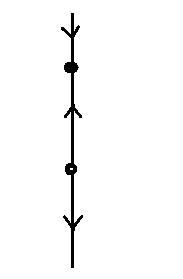
\includegraphics[width=\linewidth]{images/1.6-Phase1.png}
\end{image}%
\tcblower
\end{figureptx}%
For example, the phase line shows that as \(y\) is close to \(y=1\) from below, then the function keeps increasing, and thus must approach asymptotically to the equilibrium solution.%
\par
A sketch of some possible solutions looks like: \begin{figureptx}{Solution sketch for \(\frac{dy}{dt} = y(1-y)\)}{x:figure:fig-sketch1}{}%
\begin{image}{0.3}{0.4}{0.3}%
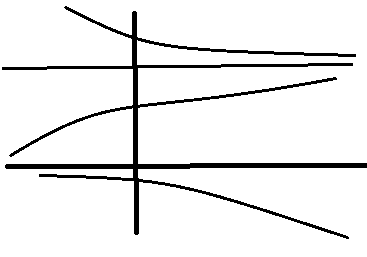
\includegraphics[width=\linewidth]{images/1.6-Sketch1.png}
\end{image}%
\tcblower
\end{figureptx}%
%
\par
From our first sketch we can always notice the following things about sketching curves:%
%
\begin{enumerate}
\item{}If \(f(y(0))=0\) then \(y(0)\) is an equilibirum solution and \(y(t)=y(0)\) for all \(t\).%
\item{}If \(f(y(0))>0\) then \(y(t)\) is \emph{increasing} for all \(t\) and either \(y(y)\to\infty\) as \(t\to\infty\) or \(y(t)\) tends to first equilibirum point \emph{larger} than \(y(0).\)%
\item{}If \(f(y(0))
\lt 0\) then then \(y(t)\) is \emph{decreasing} for all \(t\) and either \(y(y)\to-\infty\) as \(t\to\infty\) or \(y(t)\) tends to first equilibirum point \emph{smaller} than \(y(0).\)%
\end{enumerate}
\begin{example}{Curve Sketching.}{g:example:idm45282412004320}%
We let%
\begin{equation*}
\frac{dy}{dt}=(2-y)\sin y.
\end{equation*}
%
%
\begin{enumerate}
\item{}Find equilibrium points \(y=2\) and \(y=n\pi\) (so infinite amount)%
\item{}Plug points and get that the phase line is : \begin{image}{0.35}{0.3}{0.35}%
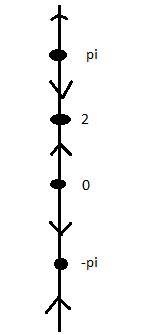
\includegraphics[width=\linewidth]{images/1.6-Phase2.png}
\end{image}%
%
\item{}Talk about what happens when things are getting close to the equilibrium solutions.%
\item{}Sketch curves: \begin{image}{0}{1}{0}%
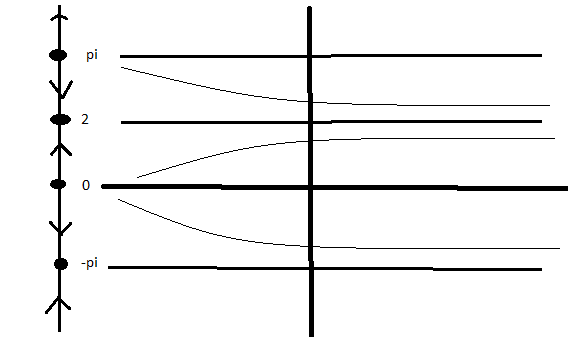
\includegraphics[width=\linewidth]{images/1.6-Sketch2.png}
\end{image}%
%
\end{enumerate}
\end{example}
\begin{example}{We don't know how quickly things jump.}{g:example:idm45282411997984}%
Show that the graph \(\frac{dP}{dt}=(1-\frac{P}{20})^{3}(\frac{P}{5}-1)P^{7}\) has Phase line \([\ominus20\oplus5\ominus0\oplus]\)\(\begin{array}{c}
\vee\\
20\\
\wedge\\
5\\
\vee\\
0\\
\wedge
\end{array}\) but \(5\) jumps to \(20\) very quickly (like \(0.00001\) quick.%
\begin{sageinput}
t,y=var('t,y')
plot_slope_field((1 - y/20)^3 * (y/5 - 1) *y^7, (t,-5,5), (y,0, 20))
\end{sageinput}
\end{example}
\begin{example}{Not all solutions exist for all \(t\).}{g:example:idm45282411992960}%
Consider the equation \(\frac{dy}{dt}=(1+y)^{2}\).%
\par
The phase line is \([\ominus-1\oplus]\) \(\begin{array}{c}
\wedge\\
-1\\
\wedge
\end{array}\) Sketch a curve.%
\par
These increasing\slash{}decreasing behaviors could be asymptotes. (Phase LINE DOES NOT TELL US THIS INFO)%
\par
ACTUAL SOL: \(y(t)=-1-\frac{1}{t+c}\). Asymptote at \(t=c\).%
\par
If \(y(0)>-1\) then draw possible curve.%
\begin{sageinput}
t,y=var('t,y')
g = Graphics()
g+= plot_slope_field((1+y)^2, (t,-5,5),(y,-5,5))
g+= plot(-1-1/(t + 2), (t,-5,5), ymax = 5, ymin = -5)
g.show()
\end{sageinput}
\end{example}
\begin{example}{Cusps.}{g:example:idm45282411985568}%
Consider the equation \(\frac{dy}{dt}=\frac{1}{1-y}\).%
\par
The phase line would be: \begin{image}{0}{1}{0}%
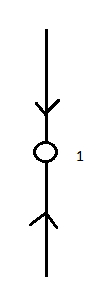
\includegraphics[width=\linewidth]{images/1.6-Phase3.png}
\end{image}%
 We can sketch ``cusp-like'' curves. Once a curve has fallen into a hole once it reaches the dotted line.%
\begin{sageinput}
t,y=var('t,y')
g = Graphics()
g+= plot_slope_field(1/(1-y), (t, -5, 5), (y, -5, 5))
g+= plot(1 + sqrt(-2*t + 4), (t, -5, 2))
g+= plot(1 - sqrt(-2*t -2), (t, -5, -1), color="red")
g.show()
\end{sageinput}
\end{example}
\alert{Role of Equilibrium points:}%
\par
The solutions to autonomous equations either%
\begin{enumerate}
\item{}Tend to \(\pm\infty\)%
\item{}Tend to the equilibrium solutions.%
\item{}Stay consistently increasing\slash{}decreasing within equilibrium solutions.%
\end{enumerate}
%
\end{subsectionptx}
%
%
\typeout{************************************************}
\typeout{Subsection 2.7.3 Classification of Equilibrium Solutions}
\typeout{************************************************}
%
\begin{subsectionptx}{Classification of Equilibrium Solutions}{}{Classification of Equilibrium Solutions}{}{}{g:subsection:idm45282411977872}
Recall what \terminology{asymptotic} means: say that \(f\) is asymptotic to the line \(y = c\) if%
\begin{equation*}
\lim_{t \to \infty} f(t) = c.
\end{equation*}
%
\par
We can classify the equilibrium solutions to an autonomous equation by looking at the behavior of ``nearby'' solutions. Solutions fall into one of three categories.%
%
\begin{enumerate}
\item{}\alert{Asymptotically stable (sink)}%
%
\begin{enumerate}
\item{}\(y_{0}\) is an \terminology{asymptotically stable} equilibrium if any solution with initial condition sufficiently close to \(y_{0}\) is asymptotic to \(y_{0}\) as \(t\) increases.%
\item{}Phase Line looks like this: \(\left[\ominus y_{0}\oplus\right]\) \(\begin{array}{c}
\vee\\
y_{0}\\
\wedge
\end{array}\)%
\item{}Graph looks like: (reminds you that it is falling into something)%
\item{}In a graph of \(f(y)\) vs. \(y\), we have \(f^{\prime}(y_{0}) \lt 0\).%
\end{enumerate}
\item{}\alert{Asymptotically unstable (source):}%
%
\begin{enumerate}
\item{}\(y_{0}\) is an \terminology{asymptotically unstable} equilibrium if any solution with initial condition sufficiently close to \(y_{0}\) tends torward \(y_{0}\) as \(t\) decreases.%
\item{}The phase line looks like this: \(\left[\oplus y_{0}\ominus\right]\) \(\begin{array}{c}
\wedge\\
y_{0}\\
\vee
\end{array}\)%
\item{}Graph looks like: ( reminds you that it is coming from one place)%
\item{}In \(f(y)\) vs. \(y\) graph, we have \(f^{\prime}(y_{0})>0\).%
\end{enumerate}
\item{}\alert{Semistable:}%
%
\begin{enumerate}
\item{}\(y_{0}\) is an \alert{asymptotically semistable} equilibrium if it doesn't fit the category of a sink or source \textbackslash{}item Phase Line looks like this: \(\left[\oplus y_{0}\oplus\right]\) \(\begin{array}{c}
\wedge\\
y_{0}\\
\wedge
\end{array}\)or \(\left[\ominus y_{0}\ominus\right]\) \(\begin{array}{c}
\vee\\
y_{0}\\
\vee
\end{array}\)%
\item{}Graph looks like:%
\end{enumerate}
\end{enumerate}
\begin{example}{Drawing solution from the \(f(y)\) vs. \(y\) graph).}{g:example:idm45282411952944}%
Consider the equation \(\frac{dy}{dt}=y^{2}+y-6=(y+3)(y-2)\).%
\par
The phase line is \(\left[\oplus2\ominus-3\oplus\right]\) \(\begin{array}{c}
\wedge\\
2\\
\vee\\
-3\\
\wedge
\end{array}\)%
\par
How can these be classified?%
\end{example}
\begin{example}{(Using \(f(y)\)).}{g:example:idm45282411948640}%
We can figure out classification directly from the graph of \(f(y)\). \begin{image}{0}{1}{0}%
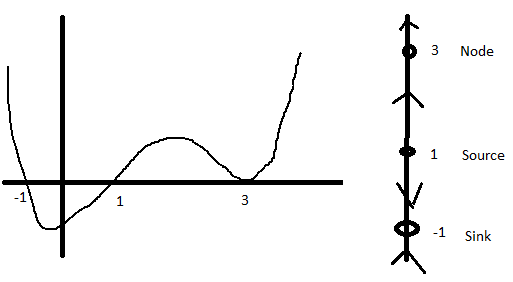
\includegraphics[width=\linewidth]{images/1.6-Classif-1.png}
\end{image}%
 Here, node means semistable, sink means stable, and source means unstable.%
\end{example}
\begin{example}{}{g:example:idm45282411945712}%
Suppose we only know the graph of \(f(y)\) not the actual formula. \begin{image}{0}{1}{0}%
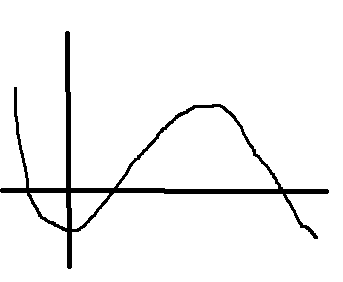
\includegraphics[width=\linewidth]{images/1.6-f(y).png}
\end{image}%
 Then draw phase line : \(\left[\ominus c\oplus b\ominus a\oplus\right]\) \(\begin{array}{c}
\vee\\
c\\
\wedge\\
b\\
\vee\\
a\\
\wedge
\end{array}\) Now sketch some solution curves.%
%
\end{example}
\end{subsectionptx}
\end{sectionptx}
%
%
\typeout{************************************************}
\typeout{Section 2.8 Exact equations}
\typeout{************************************************}
%
\begin{sectionptx}{Exact equations}{}{Exact equations}{}{}{x:section:ch2-8}
\begin{introduction}{}%
This section introduces a family of equations that arise naturally in physical contexts. For example, suppose that we had a detailed temperature map of a hot metal sheet. Can we predict how the heat will flow? The answer to this question is provided by the gradient, studied in multi-variable calculus. But what about the opposite scenario? Given a heat flow map, can we reconstruct the original temperature distribution? To answer this question, we'll consider what are known as \terminology{exact equations}. First, we recall some multivariable calculus.%
\end{introduction}%
%
%
\typeout{************************************************}
\typeout{Subsection 2.8.1 Partial derivatives and the gradient}
\typeout{************************************************}
%
\begin{subsectionptx}{Partial derivatives and the gradient}{}{Partial derivatives and the gradient}{}{}{g:subsection:idm45282411939024}
Suppose that \(z = f(x,y)\) is a function of two independent variables. Just as in one variable, we want to understand how the graph of \(f\) changes at a point, but now we have lots of different directions to look at. To compute the rate of change in the \(x\) and \(y\) directions, we can use the \terminology{partial derivative} in those directions. When we take a partial derivative with respect to a variable, we treat all other variables as constant so that we're isolating our view to change in that specific direction.%
\begin{definition}{}{g:definition:idm45282411935200}%
Let \(z = f(x,y)\). The partial derivative of \(f\) with respect to \(x\) is%
\begin{equation*}
\frac{\partial f}{\partial x} = \lim_{h \to 0} \frac{f(x + h, y) - f(x,y)}{h}.
\end{equation*}
The partial derivative of \(f\) with respect to \(y\) is%
\begin{equation*}
\frac{\partial f}{\partial y} = \lim_{h\to 0}\frac{f(x, y+h) - f(x,y)}{h}.
\end{equation*}
%
\end{definition}
In practice, we can use the single variable differentiation rules, treating the other variable like it is a fixed number. For example,%
\begin{equation*}
\frac{\partial}{\partial x} x^2 + x \cos y + y^2 = 2x + \cos y + 0.
\end{equation*}
%
\par
Frequently, when given a function \(z = f(x,y)\), we wish to know the direction of greatest slope or rate of change. For example, if \(z = f(x,y)\) represents the height of a mountain, the direction that water flows downhill will be in the direction of sleepest descent. We can use the partial derivatives to define a \terminology{vector field} that at each point \((x,y)\) gives the direction of greatest slope of the graph of \(f\).%
\begin{definition}{}{g:definition:idm45282411927248}%
The \terminology{gradient} of \(z = f(x,y)\) is the vector-valued function%
\begin{equation*}
\nabla f = \langle \frac{\partial f}{\partial x}, \frac{\partial f}{\partial y}\rangle.
\end{equation*}
This is written shorthand as \(\nabla f = \langle f_x, f_y\rangle\).%
\end{definition}
You should think of the gradient in this context as a slope field - at every point in the \(x-y\) plane, the gradient attaches a vector that indicates the direction of greatest slope.%
\par
If we think of \(z = f(x,y)\) as a voltage map or a temperature map or a height map, a standard visualization is to use curves to represent points that have equal heights. Such curves are called \terminology{isotherms} or \terminology{equipotential lines} or altitude lines.%
\begin{example}{Equipotentials and surfaces.}{g:example:idm45282411921440}%
Let \(f(x, y) = -x^2 + 3y - y^2\). The following code will plot some equipotentials of \(f\). In particular, we will plot the curves corresponding to \(z = 0, 1, 2\).%
\begin{sageinput}
x,y = var('x,y')
g = Graphics()
g+= implicit_plot(-x^2  + 3*y - y^2, (x, -2,2), (y, 0,3), color = "red" )
g+=implicit_plot(-x^2  + 3*y - y^2 - 1, (x, -2,2), (y, 0,3), color="yellow" )
g+= implicit_plot(-x^2  + 3*y - y^2-2, (x, -2,2), (y, 0,3), color="green" )
g.show()
\end{sageinput}
 Now compare to the surface itself: \begin{sageinput}
var('x y z')
f(x, y) = -x^2  + 3*y - y^2
P = implicit_plot3d(f-z, (x ,-1, 3), (y, 0, 3), (z, -2, 3))
Q = plot3d(0, (-1,3), (0,3), color="red", opacity=".4")
R = plot3d(1, (-1,3), (0,3), color="yellow", opacity = ".4")
S = plot3d(2, (-1,3), (0,3), color ="green", opacity = ".4")
P + Q +R +S
\end{sageinput}
\end{example}
\begin{example}{Relationship between equipotentials and gradients.}{g:example:idm45282411916272}%
One of the most important geometric facts about the relationship between the \terminology{potential function} \(f\) and the gradient field \(\nabla f\) is that \emph{equipotentials are perpendicular to gradients.} Using our previous example:%
\begin{sageinput}
x,y = var('x,y')
g = Graphics()
g+= implicit_plot(-x^2  + 3*y - y^2, (x, -2,2), (y, 0,3), color = "red" )
g+=implicit_plot(-x^2  + 3*y - y^2 - 1, (x, -2,2), (y, 0,3), color="yellow" )
g+= implicit_plot(-x^2  + 3*y - y^2-2, (x, -2,2), (y, 0,3), color="green" )
g+= plot_vector_field((-2*x, 3 - 2*y), (-2,2), (0,3))
g.show()
\end{sageinput}
\end{example}
In summary, given a \terminology{potential function} \(z = f(x,y)\),%
\begin{enumerate}
\item{}We can find the equipotential lines (lines of constant height)%
\begin{equation*}
C = f(x,y);
\end{equation*}
%
\item{}we can find the gradient field%
\begin{equation*}
\nabla f = \langle f_x, f_y \rangle;
\end{equation*}
%
\item{}and we know that at a given point, the equipotential and the gradient line are perpendicular.%
\end{enumerate}
%
\end{subsectionptx}
%
%
\typeout{************************************************}
\typeout{Subsection 2.8.2 From gradient field to potential function}
\typeout{************************************************}
%
\begin{subsectionptx}{From gradient field to potential function}{}{From gradient field to potential function}{}{}{g:subsection:idm45282411907568}
How do we know when we can go the other direction? That is, as we asked at the top of the section, when given a vector field \(F(x,y) = (M(x,y), N(x,y))\), how can we recover a potential function \(f\)? Essentially, this is asking us to find a function so that \(\nabla f = F\) (the ``antiderivative of \(F\) is \(f\)''). Like integration problems, this may not always exist.%
\begin{definition}{}{g:definition:idm45282411903568}%
A vector field \(F\) is called \terminology{conservative} if there exists a potential function \(f\) so that \(\nabla f = F\).%
\end{definition}
One marker of nice functions in two variables is the conclusion of \terminology{Clairaut's theorem}, which states that the \terminology{mixed partial derivatives} of \(f\) are equal - that is, for a nice \(f\),%
\begin{equation*}
\frac{\partial^2 f}{\partial x \partial y} = \frac{\partial^2 f}{\partial y \partial x}.
\end{equation*}
Suppose for the moment that a vector field%
\begin{equation*}
F = \langle M, N \rangle = \nabla f = \langle f_x, f_y \rangle
\end{equation*}
and that the derivatives \(f_{xx}, f_{yy}, f_{xy}, f_{yx}\) all exist and are continuous. Clairaut's theorem will force%
\begin{equation*}
\frac{\partial M}{\partial y} = f_{xy} = f_{yx} = \frac{\partial N}{\partial x}\text{.}
\end{equation*}
It turns out to be the case that this condition, \(M_y = N_x\), is not only necessary but sufficient on nice enough domains like rectangles.%
\begin{theorem}{}{}{g:theorem:idm45282411895872}%
Let \(F = \langle M(x,y), N(x,y) \rangle\) be a vector field so that the partial derivatives of \(M\) and \(N\) exist and are continuous on a rectangle \(a \leq x \leq b, c \leq y \leq d\). Then there exists a potential function \(f\) so that \(\nabla f = F\) if%
\begin{equation*}
M_y = N_x.
\end{equation*}
%
\end{theorem}
\end{subsectionptx}
%
%
\typeout{************************************************}
\typeout{Subsection 2.8.3 Differential equations and equipotentials}
\typeout{************************************************}
%
\begin{subsectionptx}{Differential equations and equipotentials}{}{Differential equations and equipotentials}{}{}{g:subsection:idm45282411891536}
The \terminology{total derivative} of a function \(z = f(x,y)\) is given by the expression%
\begin{equation*}
df = f_x \, dx + f_y \, dy.
\end{equation*}
Notice that the functions that appear as components in \(df\) are the components of the gradient \(\nabla f\). If we were given the equation of an equipotential for \(f\), say%
\begin{equation*}
f(x, y) = C,
\end{equation*}
then the total derivative of the equation is%
\begin{align*}
\amp df = dC \\
\Rightarrow \amp f_x \, dx + f_y \, dy = 0\\
\Rightarrow \amp M \, dx + N \, dy = 0.
\end{align*}
If we have further that \(f\) has continuous second partial derivatives on a rectangle \(a \leq x \leq b, c \leq y \leq d\), then Clairaut's theorem gives%
\begin{equation*}
M_y = f_{xy} = f_{yx} = N_x.
\end{equation*}
%
\par
The upshot of all of this is that we can view an equation of the form%
\begin{equation*}
M \, dx + N \, dy = 0
\end{equation*}
as a differential equation that seeks to find the equipotentials \(f(x,y) = C\) for some unknown function \(f\) with \(\nabla f = \langle M, N \rangle\).%
\end{subsectionptx}
%
%
\typeout{************************************************}
\typeout{Subsection 2.8.4 Exact equations}
\typeout{************************************************}
%
\begin{subsectionptx}{Exact equations}{}{Exact equations}{}{}{g:subsection:idm45282411881120}
Consider an equation \(M(x,y)dx+N(x,y)dy=0.\) We say this equation is \terminology{exact} if \(\frac{\partial M}{\partial y}=\frac{\partial N}{\partial x};\) that is, as discussed in the previous section, the equation represents a differential equation that seeks to find equipotentials of a function \(f\) so that \(\nabla f = \langle M, N \rangle\).%
\begin{example}{}{g:example:idm45282411877440}%
Suppose \(\frac{dy}{dx}=\frac{-2x-y^{2}}{2xy}.\) We can rewrite this as \(\left(2x+y^{2}\right)dx+2xydy=0\) then \(M=2x+y^{2}\) and \(N=2xy\). Computing the partial derivatives,%
\begin{align*}
M_{y} \amp =2y\\
N_{x} \amp =2y
\end{align*}
are \(M_{y}=N_{x}\). Thus this equation is exact.\end{example}
\begin{theorem}{}{}{g:theorem:idm45282411873280}%
If \(M,N,M_{y},N_{x}\) are all continuous on a rectangle \([a,b]\times[c,d]\) and%
\begin{equation*}
M\,dx+N\,dy=0
\end{equation*}
is exact then there exists a function \(\psi\) such that%
\begin{equation*}
\psi_{x}(x,y)=M(x,y)\text{ and }\psi_{y}(x,y)=N(x,y)
\end{equation*}
and such that \(\psi(x,y)=C\) gives an implicit solution to the ODE.%
\end{theorem}
\begin{proofptx}{}{g:proof:idm45282411869696}
If \(\psi\) satisfies \(\psi_{x}=M\) and \(\psi_{y}=N\) such that \(\psi(x,y)=C\) then \(\psi\) defines a function \(y=\phi(x)\) implicitly. Then we show \(\phi(x)\) solves the ODE. Note that \(0=M(x,y)+N(x,y)y^{\prime}=\frac{\partial\psi}{\partial x}+\frac{\partial\psi}{\partial y}\frac{dy}{dx}=\frac{d}{dx}\left(\psi\left(x,\phi(x)\right)\right)\) by the multivariable chain rule. Thus if we integrate both sides%
\begin{align*}
\amp 0 =\frac{d}{dx}\left(\psi\left(x,\phi(x)\right)\right) \\
\iff\amp \int0dx=\int\frac{d}{dx}\left(\psi\left(x,\phi(x)\right)\right)dx\\
\iff \amp c=\psi\left(x,\phi(x)\right),
\end{align*}
as needed.\end{proofptx}
\alert{Solving exact equations:} If \(Mdx+Ndy=0\) is exact then%
\begin{align*}
\amp \psi_{x}=M(x,y) \amp \implies \amp \psi=\int M(x,y)dx+h(y)\\
\amp \amp \amp \Downarrow\\
\amp \psi_{y}=N(x,y) \amp \amp \psi_{y}=\frac{\partial}{\partial y}\left(\int M(x,y)dx\right)+h^{\prime}(y)
\end{align*}
and then solve for \(h(y)\).%
\par
\alert{Another way:} One may also solve it by starting with the second equation:%
\begin{align*}
\amp \psi_{x}=M(x,y) \amp \amp \psi_{x}=\frac{\partial}{\partial x}\left(\int N(x,y)dx\right)+g^{\prime}(x)\\
\amp \amp \amp \Uparrow\\
\amp\psi_{y}=N(x,y)\implies \amp \amp\psi=\int N(x,y)dy+g(x).
\end{align*}
%
\begin{example}{}{g:example:idm45282411857232}%
We know \(\left(2x+y^{2}\right)dx+2xydy=0\) is exact.%
\begin{enumerate}
\item{}Show it's exact(done earlier) and follow the arrows until you close the diagram:%
\begin{align*}
\text{Start here:} \amp \psi_{x}=2x+y^{2} \amp \implies \amp \psi=\int\left(2x+y^{2}\right)dx+h(y)\\
\amp  \amp  \amp \boldsymbol{\psi=x^{2}+y^{2}x+h(y)}\\
\amp  \amp  \amp \Downarrow\\
\amp \psi_{y}=2xy \amp \Longleftarrow \amp \psi_{y}=2xy+h^{\prime}(y)
\end{align*}
%
\item{}Solve for \(h(y)\) by noting that since%
\begin{align*}
2xy=2xy+h^{\prime}(y)\implies \amp h^{\prime}(y)=0\\
\implies \amp h(y)=C.
\end{align*}
%
\item{}Put it all together and get \(\psi(x,y)=x^{2}+y^{2}x+C\) and hence the \emph{implicit solution} is \(x^{2}+y^{2}x=C.\)%
\end{enumerate}
%
\end{example}
\begin{example}{}{g:example:idm45282411848816}%
Solve \(\left(y\cos x+2xe^{y}\right)+\left(\sin x+x^{2}e^{y}-y^{2}\right)y^{\prime}=0.\)%
\par
%
\begin{enumerate}
\item{}To show it's exact note that \(\left(y\cos x+2xe^{y}\right)dx+\left(\sin x+x^{2}e^{y}-y^{2}\right)dy=0,\) and not hard to see that%
\begin{align*}
M_{y} \amp =\cos x+2xe^{y}\\
N_{x} \amp =\cos x+2xe^{y}
\end{align*}
and they are equal, thus this ODE is exact. Follow the arrows until close the diagram:%
\begin{align*}
\text{Start here:} \amp \psi_{x}=y\cos x+2xe^{y} \amp \implies \amp \psi=\int\left(y\cos x+2xe^{y}\right)dx+h(y)\\
\amp  \amp  \amp \boldsymbol{\psi=y\sin x+x^{2}e^{y}+h(y)}\\
\amp  \amp  \amp \Downarrow\\
\amp \psi_{y}=\sin x+x^{2}e^{y}-y^{2} \amp \Longleftarrow \amp \psi_{y}=\sin x+x^{2}e^{y}+h^{\prime}(y)
\end{align*}
%
\item{}Solve for \(h(y)\) by noting that since%
\begin{align*}
\sin x+x^{2}e^{y}-y^{2}=\sin x+x^{2}e^{y}+h^{\prime}(y)\implies \amp h^{\prime}(y)=-y^{2}\\
\implies \amp h(y)=-\frac{y^{3}}{3}
\end{align*}
%
\item{}Put it all together and get \(\psi(x,y)=y\sin x+x^{2}e^{y}-y\) and hence the \emph{implicit solution} is \(y\sin x+x^{2}e^{y}-\frac{y^{3}}{3}=C.\)%
\end{enumerate}
%
\begin{sageinput}
var('x,y')
P = plot_vector_field((y*cos(x) + 2*x*e^y, sin(x) + x^2*e^y - y^2), (-3,3),(-3,3))
Q = implicit_plot(y *sin(x) + x^2*e^y - y^3/3 - 5,(-3,3),(-3,3), color="red")
R = implicit_plot(y *sin(x) + x^2*e^y - y^3/3 - 3,(-3,3),(-3,3), color ="orange")
S = implicit_plot(y *sin(x) + x^2*e^y - y^3/3,(-3,3),(-3,3), color ="blue")
P + Q +R +S
\end{sageinput}
\end{example}
\begin{example}{}{g:example:idm45282411837152}%
Find the value of \(b\) for which the given equation is exact, and then solve it using that \(b\): \(\left(xy^{2}+bx^{2}y\right)dx+\left(x+y\right)x^{2}dy\)%
\begin{enumerate}
\item{}If this equation is exact then \(M_{y}=N_{x}\),%
\begin{align*}
M_{y} \amp =2xy+bx^{2}\\
N_{x} \amp =3x^{2}+2yx
\end{align*}
and are only equal when \(b=3\). Follow the arrows until close the diagram:%
\begin{align*}
\text{Start here:} \amp \psi_{x}=xy^{2}+3x^{2}y \amp \implies \amp \psi=\int\left(xy^{2}+3x^{2}y\right)dx+h(y)\\
\amp  \amp  \amp \boldsymbol{\psi=\frac{1}{2}x^{2}y^{2}+x^{3}y+h(y)}\\
\amp  \amp  \amp \Downarrow\\
\amp \psi_{y}=x^{3}+x^{2}y \amp \Longleftarrow \amp \psi_{y}=x^{2}y+x^{3}+h^{\prime}(y)
\end{align*}
%
\item{}Solve for \(h(y)\) by noting that since%
\begin{align*}
x^{3}+x^{2}y=x^{2}y+x^{3}+h^{\prime}(y)\implies \amp h^{\prime}(y)=0\\
\implies \amp h(y)=C
\end{align*}
%
\item{}Put it all together and get \(\psi(x,y)=\frac{1}{2}x^{2}y^{2}+x^{3}y+C\) and hence the \emph{implicit solution} is \(\frac{1}{2}x^{2}y^{2}+x^{3}y=C.\)%
\end{enumerate}
\end{example}
\begin{example}{}{g:example:idm45282411826032}%
Solve \(\left(x\cos x+e^{y}\right)dx+xe^{y}dy\)%
%
\begin{enumerate}
\item{}If this equation is exact then \(M_{y}=N_{x}\), and%
\begin{align*}
M_{y} \amp =e^{y}\\
N_{x} \amp =e^{y}
\end{align*}
Now note that it is actually easier to integrate \(N\) with respect to \(y\): Thus we can start the diagram in the other direction%
\begin{align*}
\amp \psi_{x}=x\cos x+e^{y} \amp \Longleftarrow \amp =\psi_{x}=e^{y}+g^{\prime}(x)\\
\amp  \amp  \amp \boldsymbol{\psi=xe^{y}+g(x)}\\
\amp  \amp  \amp \Uparrow\\
\text{Start here:} \amp \psi_{y}=xe^{y} \amp \implies \amp \psi_{y}=\int\left(xe^{y}\right)dy+g(x)
\end{align*}
%
\item{}Solve for \(g(x)\) by noting that since%
\begin{align*}
x\cos x+e^{y}=e^{y}+g^{\prime}(x)\implies \amp g^{\prime}(x)=x\cos x
\end{align*}
but at the end of the day we can't avoid the harder integration, as we still need to integration by parts to \(g(x)=x\sin x+\cos x\)%
\item{}Put it all together and get \(\psi(x,y)=xe^{y}+x\sin x+\cos x\) and hence the \emph{implicit solution} is \(xe^{y}+x\sin x+\cos x=C.\)%
\end{enumerate}
\begin{sageinput}
var('x,y')
P = plot_vector_field((x*cos(x) + e^y, x*e^y), (-3,3),(0,5))
Q = implicit_plot(x*e^y + x*sin(x) + cos(x) - 120,(-3,3),(0,5), color="red")
R = implicit_plot(x*e^y + x*sin(x) + cos(x) - 50,(-3,3),(0,5), color ="orange")
S = implicit_plot(x*e^y + x*sin(x) + cos(x) - 10,(-3,3),(0,5), color ="blue")
P + Q +R +S
\end{sageinput}
\end{example}
\end{subsectionptx}
\end{sectionptx}
%
%
\typeout{************************************************}
\typeout{Section 2.9 Euler's method}
\typeout{************************************************}
%
\begin{sectionptx}{Euler's method}{}{Euler's method}{}{}{x:section:ch2-9}
\begin{introduction}{}%
In practice, many if not most differential equations do not have explicit solutions. If an equation does happen to fall into a form that we have a solution method for, there is no guarantee that we can integrate the result. Thus, it is important to have approaches that can sketch curves and approximate solutions in the absence of explicit formulas.%
\par
One of the most straightforward approaches to first order equations of the form%
\begin{equation*}
\frac{dy}{dt} = f(t,y)
\end{equation*}
is \terminology{Euler's method}, which approximates a solution to an initial value problem with small pieces of tangent line.%
\par
Suppose we are given an initial value problem%
\begin{equation*}
\frac{dy}{dt}=f(t,y)\qquad y(t_{0})=y_{0}.
\end{equation*}
%
%
\begin{itemize}[label=\textbullet]
\item{}Let \(h=\) step size. These are our \(t-\)axis increments.%
\item{}Let \(t_{0}=\) our starting point. Then our next point will be \(t_{1}=t_{0}+h\), then \(t_{2}=t_{1}+h\). Notice that this means%
\begin{equation*}
t_{k+1} - t_k = h.
\end{equation*}
%
\end{itemize}
For example suppose \(t_{0}=1\) and \(h=.5\), then \(t_{0}=1,t_{1}=1.5,t_{2}=2,\dots\). So how do we find the explicit values for \(y_{k}\) other than just guessing?%
\begin{observation}{}{g:observation:idm45282411802080}%
For small step size \(h\), the slope of the tangent line at \((t_0, y_0)\) is a reasonable approximation for the secant line connecting \((t_0, y(t_0))\) to the point \((t_1), y(t_1)\). That is,%
\begin{equation*}
\frac{y(t_{k+1}) - y(t_k)}{t_{k+1} - t_k} = \frac{y(t_{k+1}) - y(t_k)}{h} \approx f(t_k, y(t_k)).
\end{equation*}
\end{observation}
Let \(y_0 = y(t_0)\). Now, denote by \(y_1\) the \emph{approximation} of \(y(t_1)\) given by%
\begin{equation*}
y(t_1) \approx y_1 := y_0 + f(t_0, y_0) h.
\end{equation*}
Iteration of this idea to produce a larger approximate graph of a solution is the key idea of Euler's method.%
\end{introduction}%
%
%
\typeout{************************************************}
\typeout{Subsection 2.9.1 Euler's method}
\typeout{************************************************}
%
\begin{subsectionptx}{Euler's method}{}{Euler's method}{}{}{g:subsection:idm45282411796240}
\begin{definition}{}{g:definition:idm45282411795504}%
Given an initial condition \(y(t_{0})=y_{0}\) and step size \(h\), compute \(\left(t_{k+1},y_{k+1}\right)\) from the preceding point \((t_{k},y_{k})\) as follows:%
\begin{align*}
t_{k+1} \amp = \amp t_{k}+h\\
y_{k+1} \amp = \amp y_{k}+f\left(t_{k},y_{k}\right)h.
\end{align*}
%
\end{definition}
\begin{example}{}{g:example:idm45282411791520}%
Suppose we have the autonomous equation%
\begin{align*}
\frac{dy}{dt}=2y-1 \amp  \amp ,y(0)=1,
\end{align*}
with \(h=0.1\) and \(0\leq t\leq1\).%
%
\begin{enumerate}
\item{}Our first point is \((t_{0},y_{0})=\left(0,1\right)\).%
\item{}We can compute the formula for this and get \(t_{k+1}=t_{k}+.1\) and notice that \(f\left(t,y\right)=2y-1\).%
\begin{equation*}
y_{k+1}=y_{k}+f\left(t_{k},y_{k}\right)h=y_{k}+\left(2y_{k}-1\right)(.1).
\end{equation*}
%
\item{}Make a table:%
\begin{equation*}
\begin{array}{|c|c|c|c|}
\hline
k \amp t_{k} \amp y_{k}=y_{k-1}+f\left(t_{k-1},y_{k-1}\right)h \amp f\left(t_{k},y_{k}\right)=2y_{k}-1\\
\hline
\hline
0 \amp 0 \amp 1 \amp 1\\
\hline
1 \amp 0.1 \amp y_{1}=1+1\cdot(.1)=\mathbf{1.1} \amp f\left(t_{1},y_{1}\right)=2(1.1)-1=\mathbf{1.20}\\
\hline
2 \amp 0.2 \amp y_{2}=1.1+(1.20)\cdot(.1)=\mathbf{1.22} \amp f\left(t_{2},y_{2}\right)=2(1.22)-1=\mathbf{1.44}\\
\hline
3 \amp 0.3 \amp y_{3}=1.22+(1.20)\cdot(.1)=\mathbf{1.364} \amp f\left(t_{3},y_{3}\right)=2(1.22)-1=\mathbf{1.73}\\
\hline
4 \amp 0.4 \amp 1.537 \amp 2.07\\
\hline
\amp .5 \amp 1.744 \amp 2.49\\
\hline
\amp .6 \amp 1.993 \amp 2.98\\
\hline
\amp .7 \amp 2.292 \amp 3.58\\
\hline
\amp .8 \amp 2.65 \amp 4.3\\
\hline
\amp 0.9 \amp 3.080 \amp 5.16\\
\hline
\amp 1.0 \amp 3.596 \amp 3.596\\
\hline
\end{array}
\end{equation*}
%
\end{enumerate}
Notice that actual value is \(y(1)=\frac{e^{2}+1}{2}=4.195\) and our approximation is \(y(1)\approx3.596\), which is a little short, but it makes sense all the slopes are always below the graph.%
\end{example}
\begin{example}{}{g:example:idm45282411782272}%
Our previous example didn't have any \(t\)s to plug in. So suppose we have%
\begin{equation*}
\frac{dy}{dt}=-2ty^{2},\quad y(0)=1,\quad h=\frac{1}{2}
\end{equation*}
%
%
\begin{enumerate}
\item{}Our first point is \((t_{0},y_{0})=\left(0,1\right)\).%
\item{}We can compute the formula for this and get \(t_{k+1}=t_{k}+.5\) and notice that \(f\left(t,y\right)=-2ty^{2}\).%
\begin{equation*}
y_{k+1}=y_{k}+f\left(t_{k},y_{k}\right)h=y_{k}+\left(-2t_{k}y_{k}^{2}\right)(\frac{1}{2}).
\end{equation*}
%
\item{}Make a table:%
\begin{equation*}
\begin{array}{|c|c|c|c|}
\hline
k \amp t_{k} \amp y_{k}=y_{k-1}+f\left(t_{k-1},y_{k-1}\right)h \amp f\left(t_{k},y_{k}\right)=-2t_{k}y_{k}^{2}\\
\hline
\hline
0 \amp 0 \amp 1 \amp 0\\
\hline
1 \amp \frac{1}{2} \amp y_{1}=1+0\cdot(\frac{1}{2})=\mathbf{1} \amp f\left(t_{1},y_{1}\right)=-2\frac{1}{2}1^{1}=\mathbf{-1}\\
\hline
2 \amp 1 \amp y_{2}=1+(-1)\cdot(\frac{1}{2})=\mathbf{\frac{1}{2}} \amp f\left(t_{2},y_{2}\right)=-2(1)(\frac{1}{2})^{2}=\mathbf{-\frac{1}{2}}\\
\hline
3 \amp 1.5=\frac{3}{2} \amp y_{3}=\frac{1}{2}+(-\frac{1}{2})\cdot(\frac{1}{2})=\frac{1}{4} \amp f\left(t_{3},y_{3}\right)=-2(\frac{3}{2})(\frac{1}{4})^{2}=\mathbf{-\frac{3}{16}}\\
\hline
4 \amp 2 \amp \frac{1}{4}+\left(-\frac{3}{16}\right)\cdot\left(\frac{1}{2}\right)=.15625 \amp \\
\hline
\end{array}
\end{equation*}
%
\end{enumerate}
A plot of our approximate solution is given below:%
\begin{image}{0}{1}{0}%
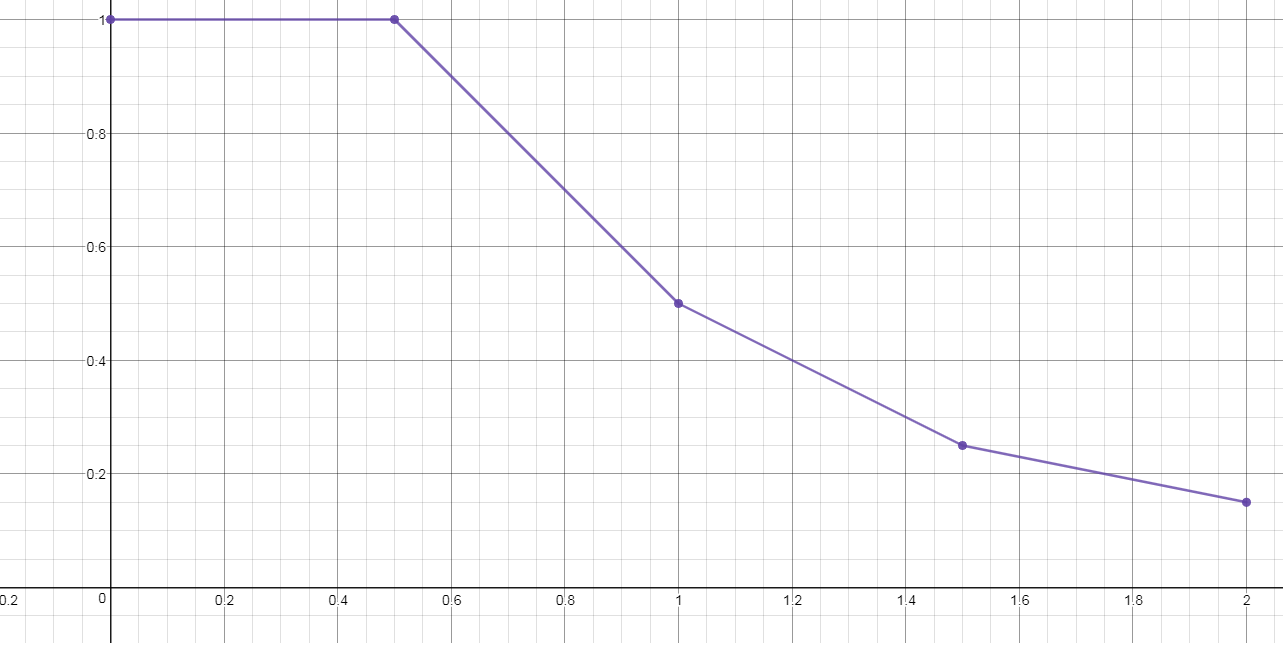
\includegraphics[width=\linewidth]{images/1.4-1.png}
\end{image}%
In code, this might look like%
\begin{sageinput}
var('t,y')
f(t, y) = -2*t*y^2
t0 = 0
y0 = 1
A = plot_slope_field(f, (0,3), (-1,3))

#approximate solution by Euler's method
h = .5
time = [t0 + n*h for n in range(5)]
yk = [y0]
def ynext(n):
    return yk[n-1] + f(time[n-1], yk[n-1])*h
for i in range(1,5):
    yk.append(ynext(i))
L = [[time[i], yk[i]] for i in range(5)]
B = line(L)

#actual solution
g(t) = 1/(t^2 + 1)
C = plot(g, (0,2), color = "red")
A + B + C
\end{sageinput}
\end{example}
\end{subsectionptx}
\end{sectionptx}
\end{chapterptx}
%
%
\typeout{************************************************}
\typeout{Chapter 3 Second Order Linear Equations}
\typeout{************************************************}
%
\begin{chapterptx}{Second Order Linear Equations}{}{Second Order Linear Equations}{}{}{x:chapter:ch3}
%
%
\typeout{************************************************}
\typeout{Section 3.1 Motivation - mass-spring systems.}
\typeout{************************************************}
%
\begin{sectionptx}{Motivation - mass-spring systems.}{}{Motivation - mass-spring systems.}{}{}{x:section:ch3-1}
\begin{introduction}{}%
This chapter is concerned with \terminology{second order differential equations}, and in particular those with \terminology{constant coefficients}. That is, we're going to be spending quite a bit of time thinking about equations of the form%
\begin{equation*}
a y'' + b y' + c y = 0
\end{equation*}
and%
\begin{equation*}
a y'' + b y' + c y = f(t).
\end{equation*}
At first glance, these equations seem artificially simple in structure. However, some of the most useful differential equations in the physical sciences and mathematics have this form, which motivates our close attention to second order linear equations with constant coefficients.%
\end{introduction}%
%
%
\typeout{************************************************}
\typeout{Subsection 3.1.1 Undamped mass-spring systems}
\typeout{************************************************}
%
\begin{subsectionptx}{Undamped mass-spring systems}{}{Undamped mass-spring systems}{}{}{g:subsection:idm45282412763312}
\begin{image}{0}{1}{0}%
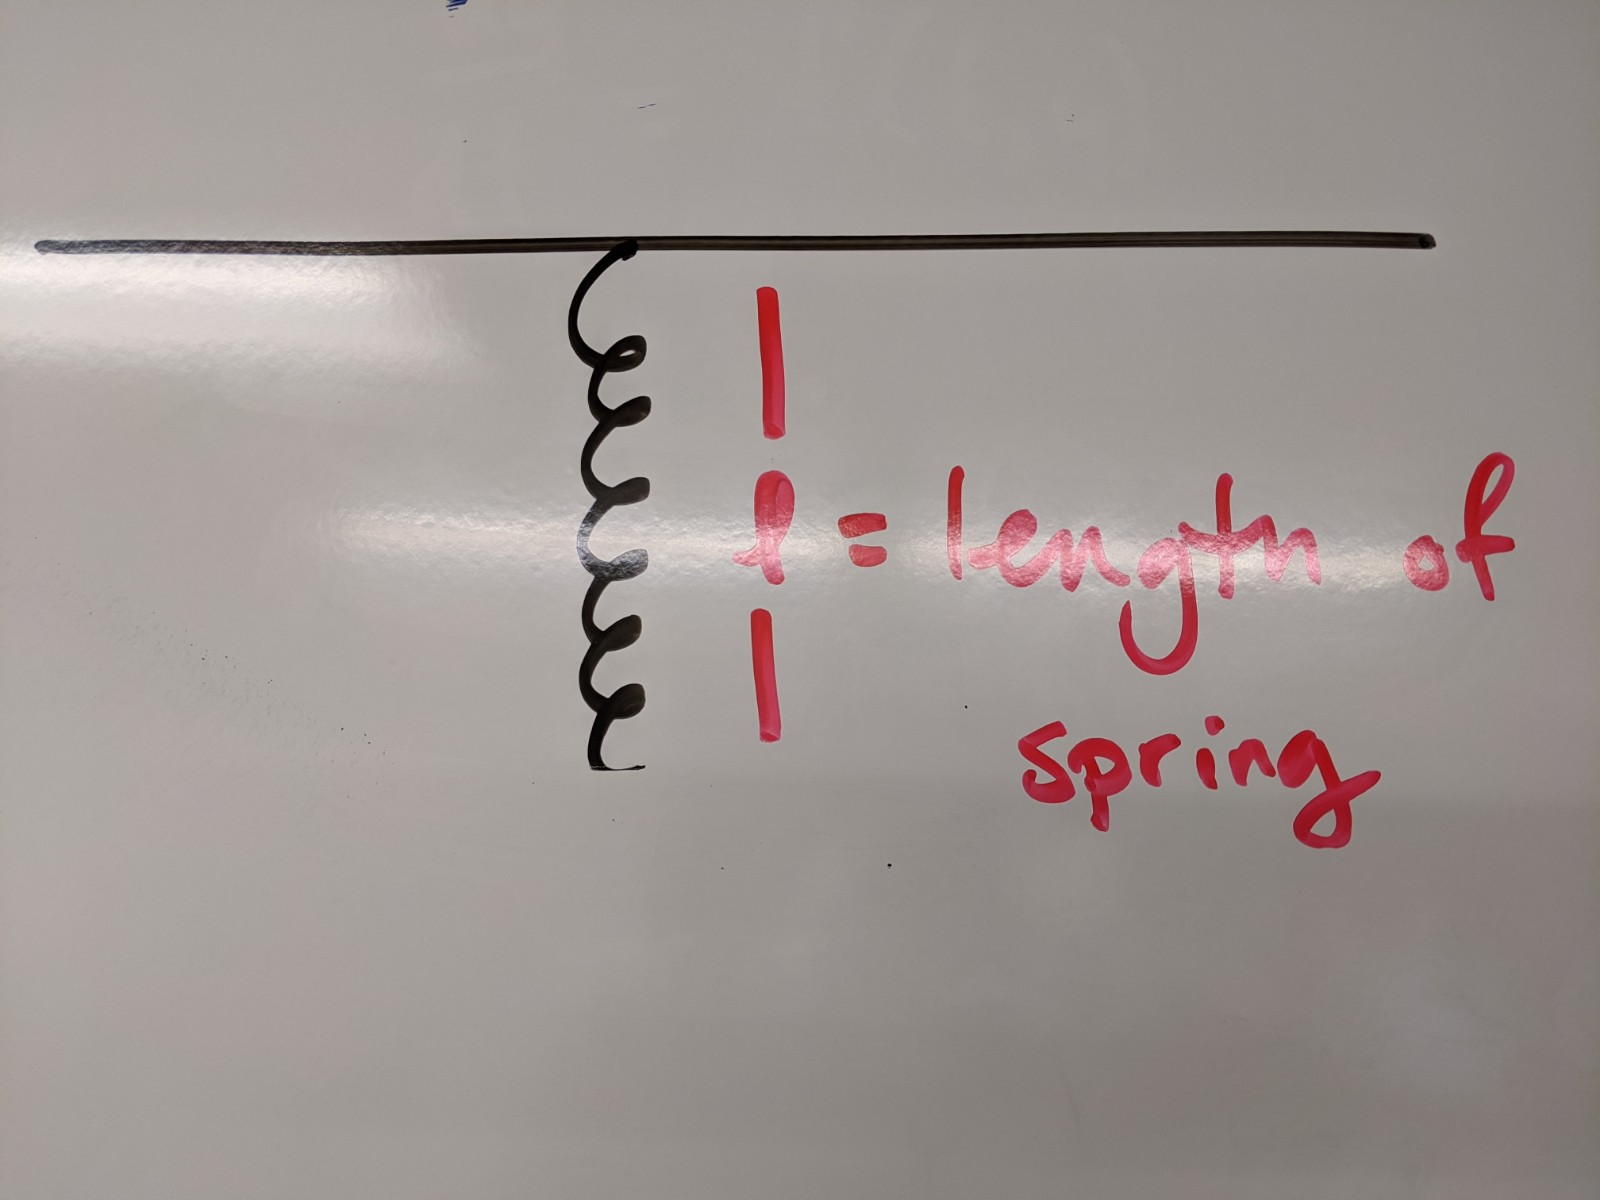
\includegraphics[width=\linewidth]{images/spring_no_mass.jpg}
\end{image}%
\begin{image}{0}{1}{0}%
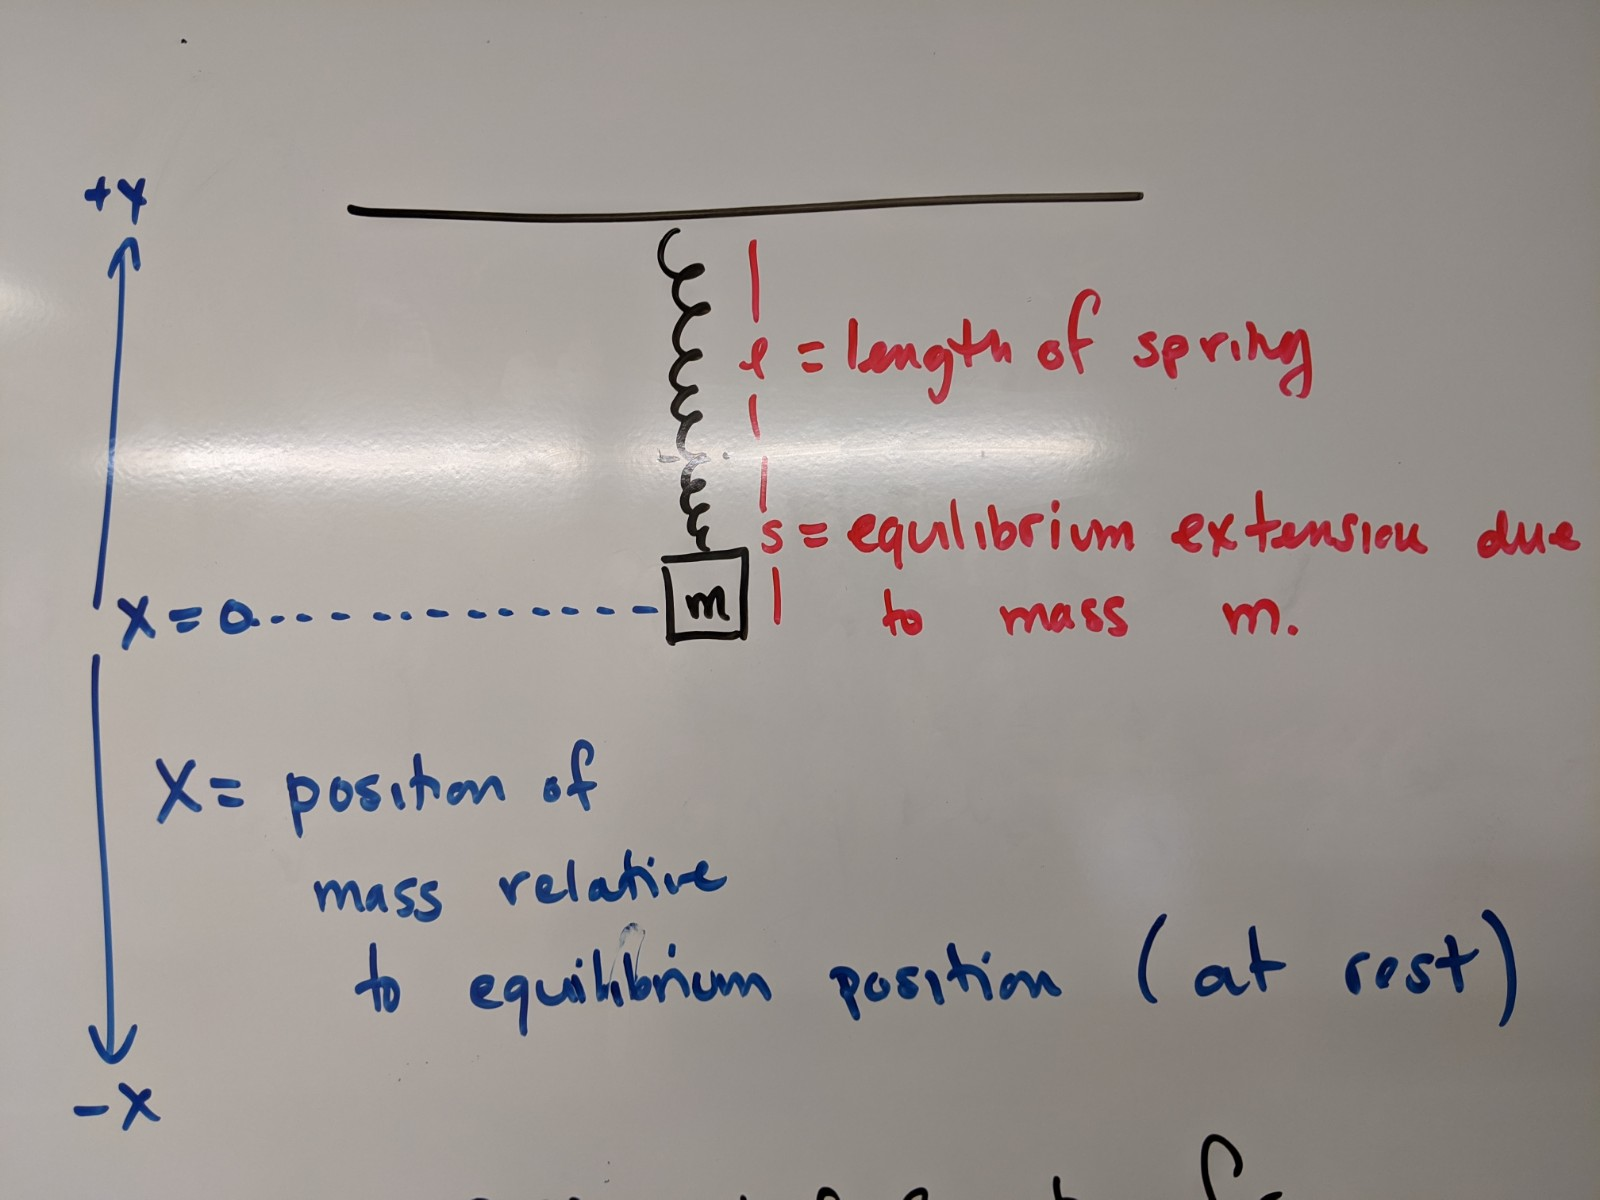
\includegraphics[width=\linewidth]{images/spring_eq.jpg}
\end{image}%
\begin{image}{0}{1}{0}%
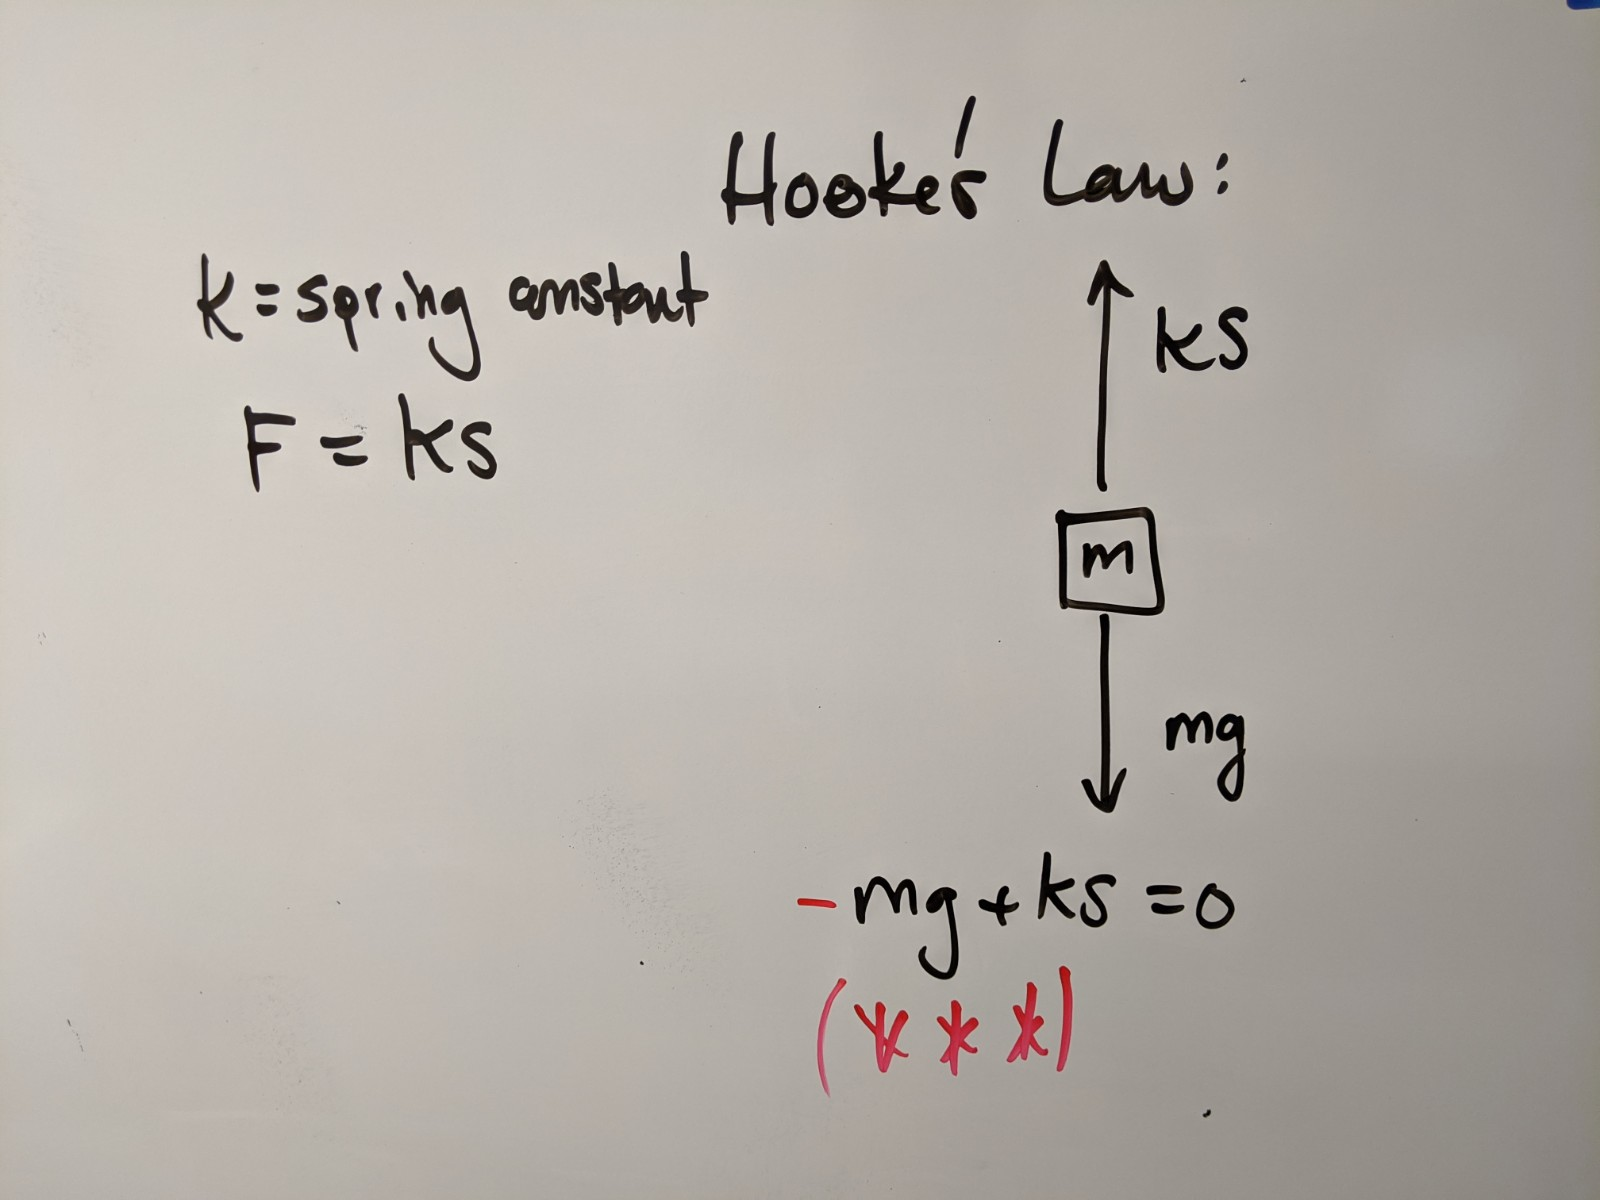
\includegraphics[width=\linewidth]{images/hookes.jpg}
\end{image}%
\begin{image}{0}{1}{0}%
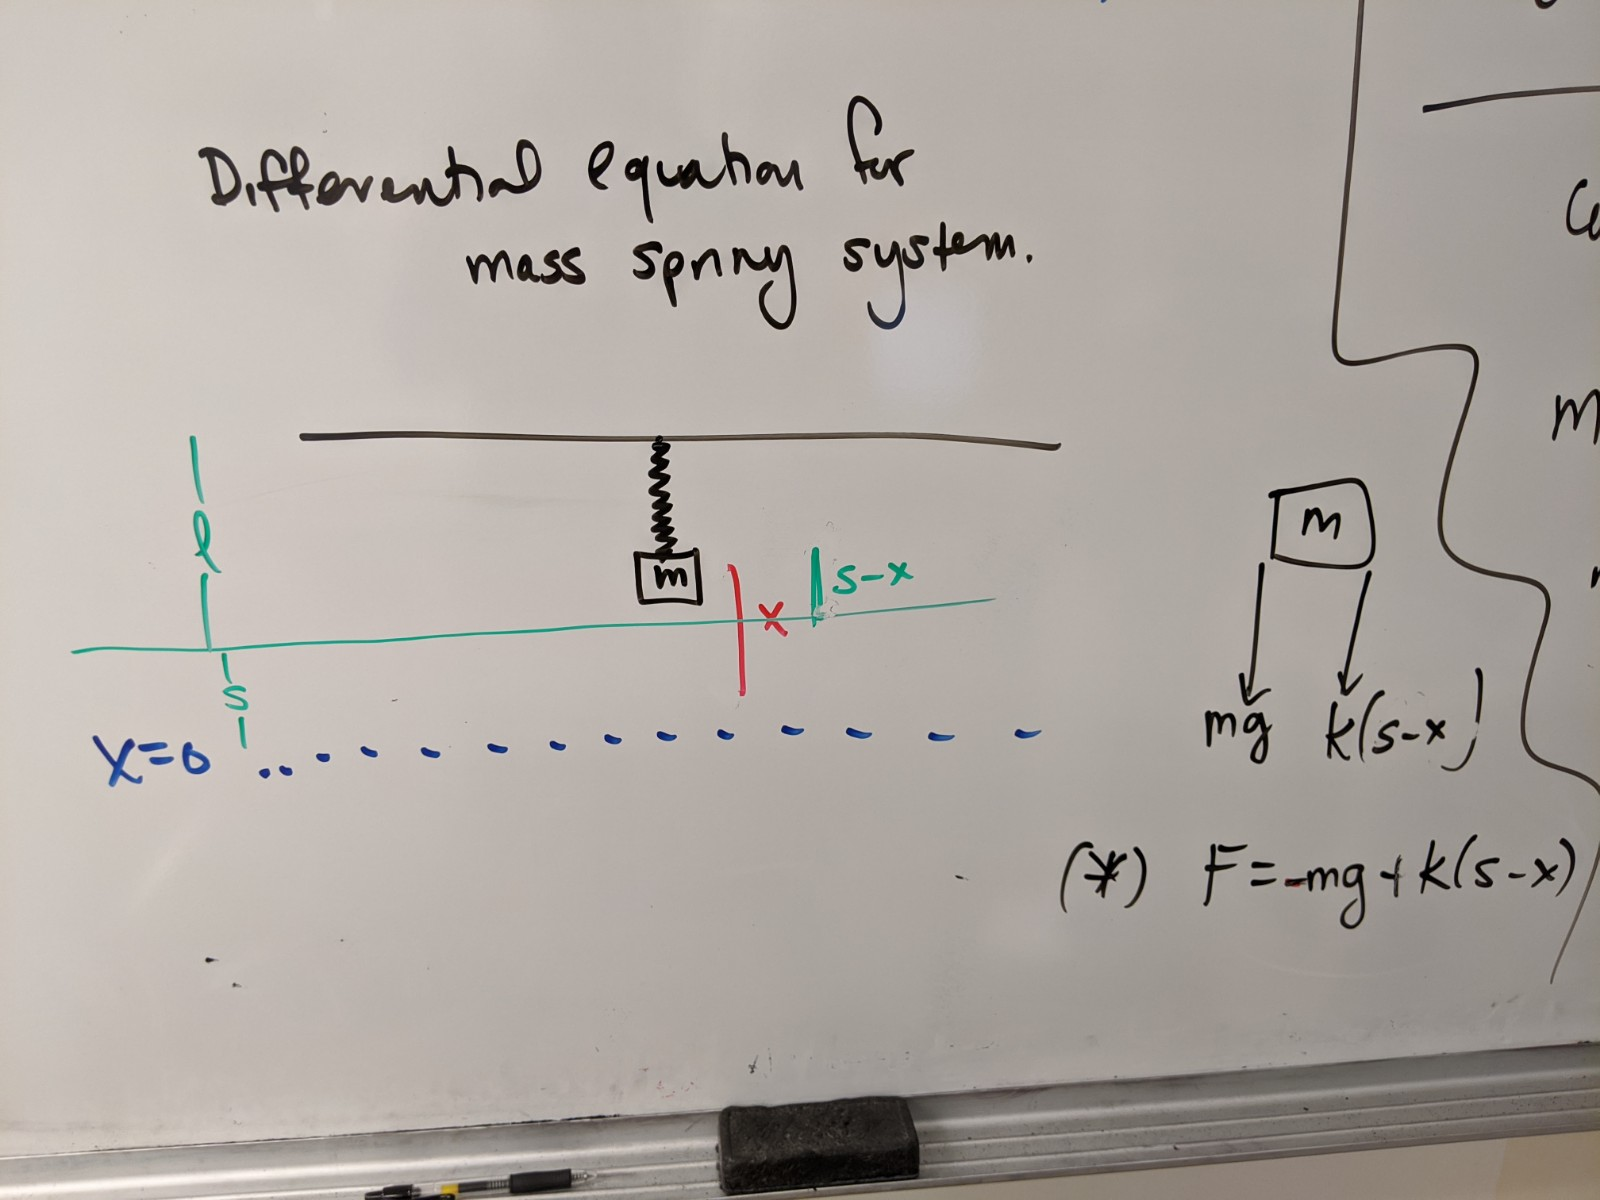
\includegraphics[width=\linewidth]{images/spring_diff_1.jpg}
\end{image}%
\begin{image}{0}{1}{0}%
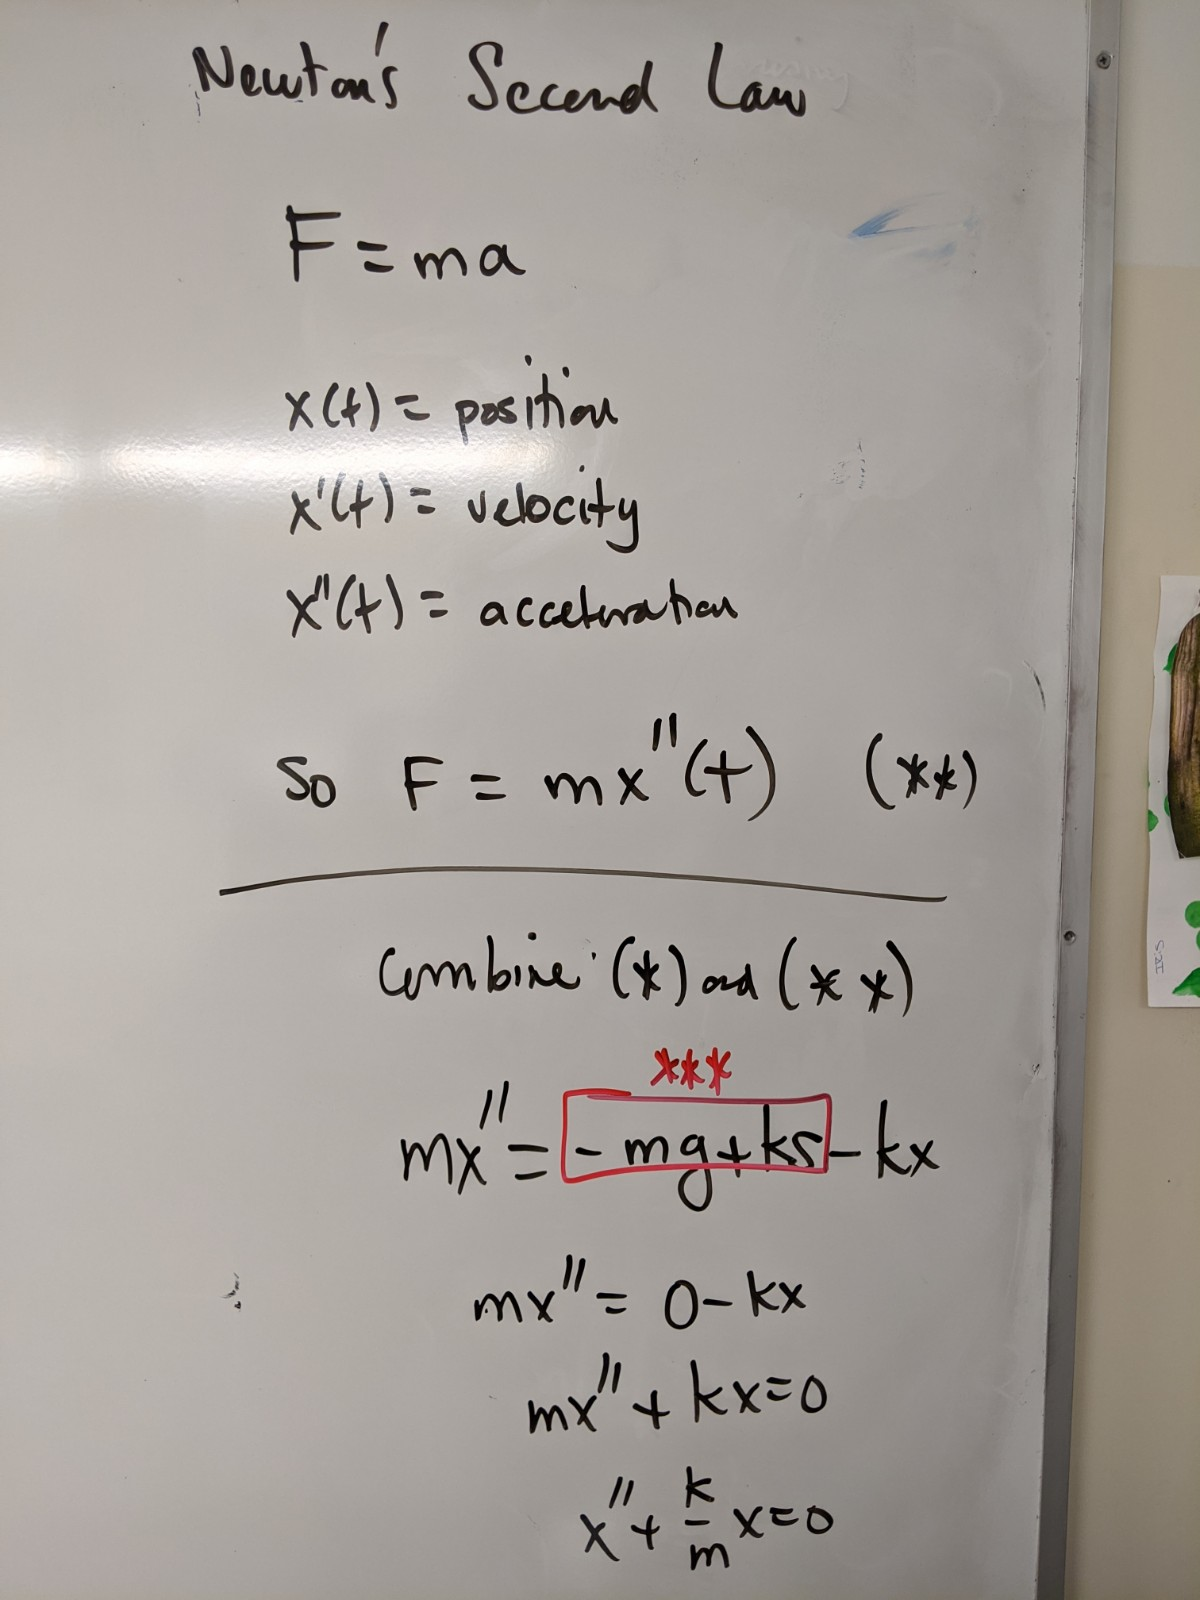
\includegraphics[width=\linewidth]{images/spring_diff_2.jpg}
\end{image}%
The pictures above are a derivation of the differential equation for a simple \terminology{mass-spring system}. Notice that the resulting equation has a second derivative \(x''\) in it - thus, this is a second order equation where the position of the mass \(x(t)\) relative to the equilibrium position is a function of time \(t\):%
\begin{equation*}
x'' + \frac{k}{m} x = 0.
\end{equation*}
Also, note the important fact that the equation is linear and has constant coefficients. If we want to describe how the solutions to this equation behave, we should study second order equations with constant coefficients.%
\end{subsectionptx}
%
%
\typeout{************************************************}
\typeout{Subsection 3.1.2 Damped mass-spring systems}
\typeout{************************************************}
%
\begin{subsectionptx}{Damped mass-spring systems}{}{Damped mass-spring systems}{}{}{g:subsection:idm45282412837472}
One way to model more complicated situations with a mass-spring system is to include a \terminology{damper} that applies force against the direction of motion. The spring\slash{}shock absorber system in a car wheel is an example of a \terminology{damped mass-spring system}. The pictures below derive the equation for this in the case that we assume that the damper exerts a force proportional to and in the opposite direction from the velocity of the mass.%
\begin{image}{0}{1}{0}%
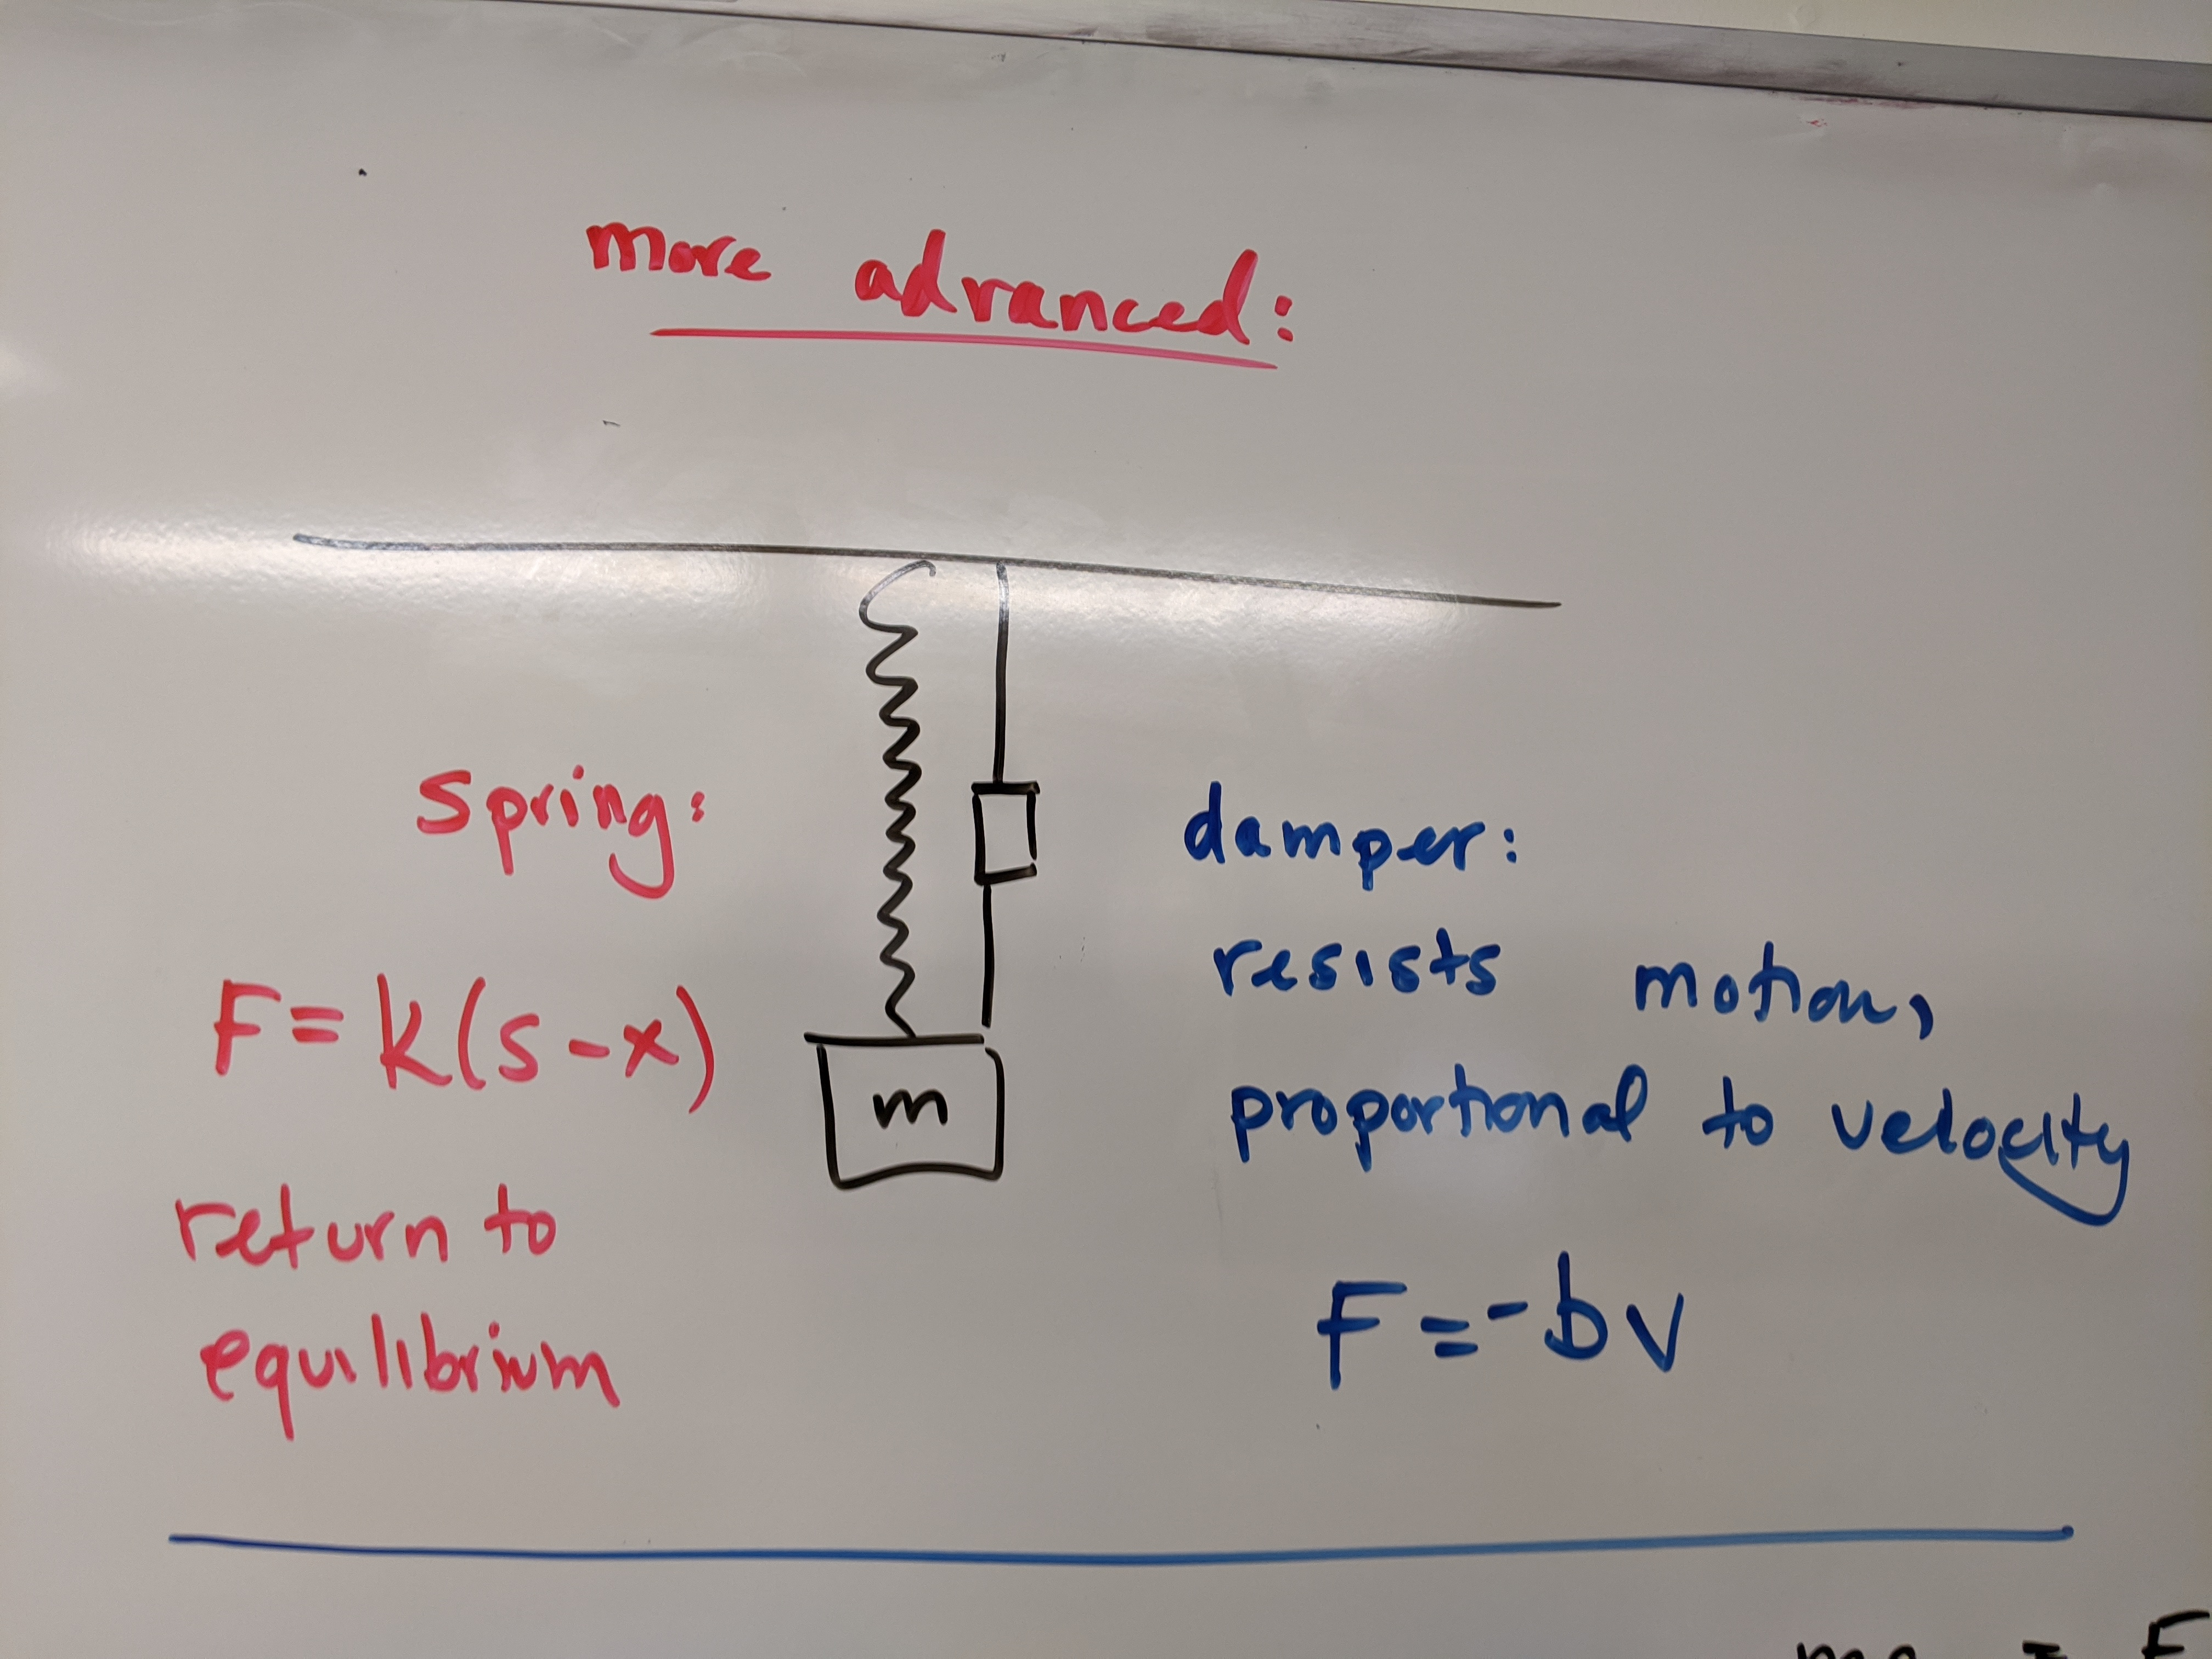
\includegraphics[width=\linewidth]{images/damped1.jpg}
\end{image}%
\begin{image}{0}{1}{0}%
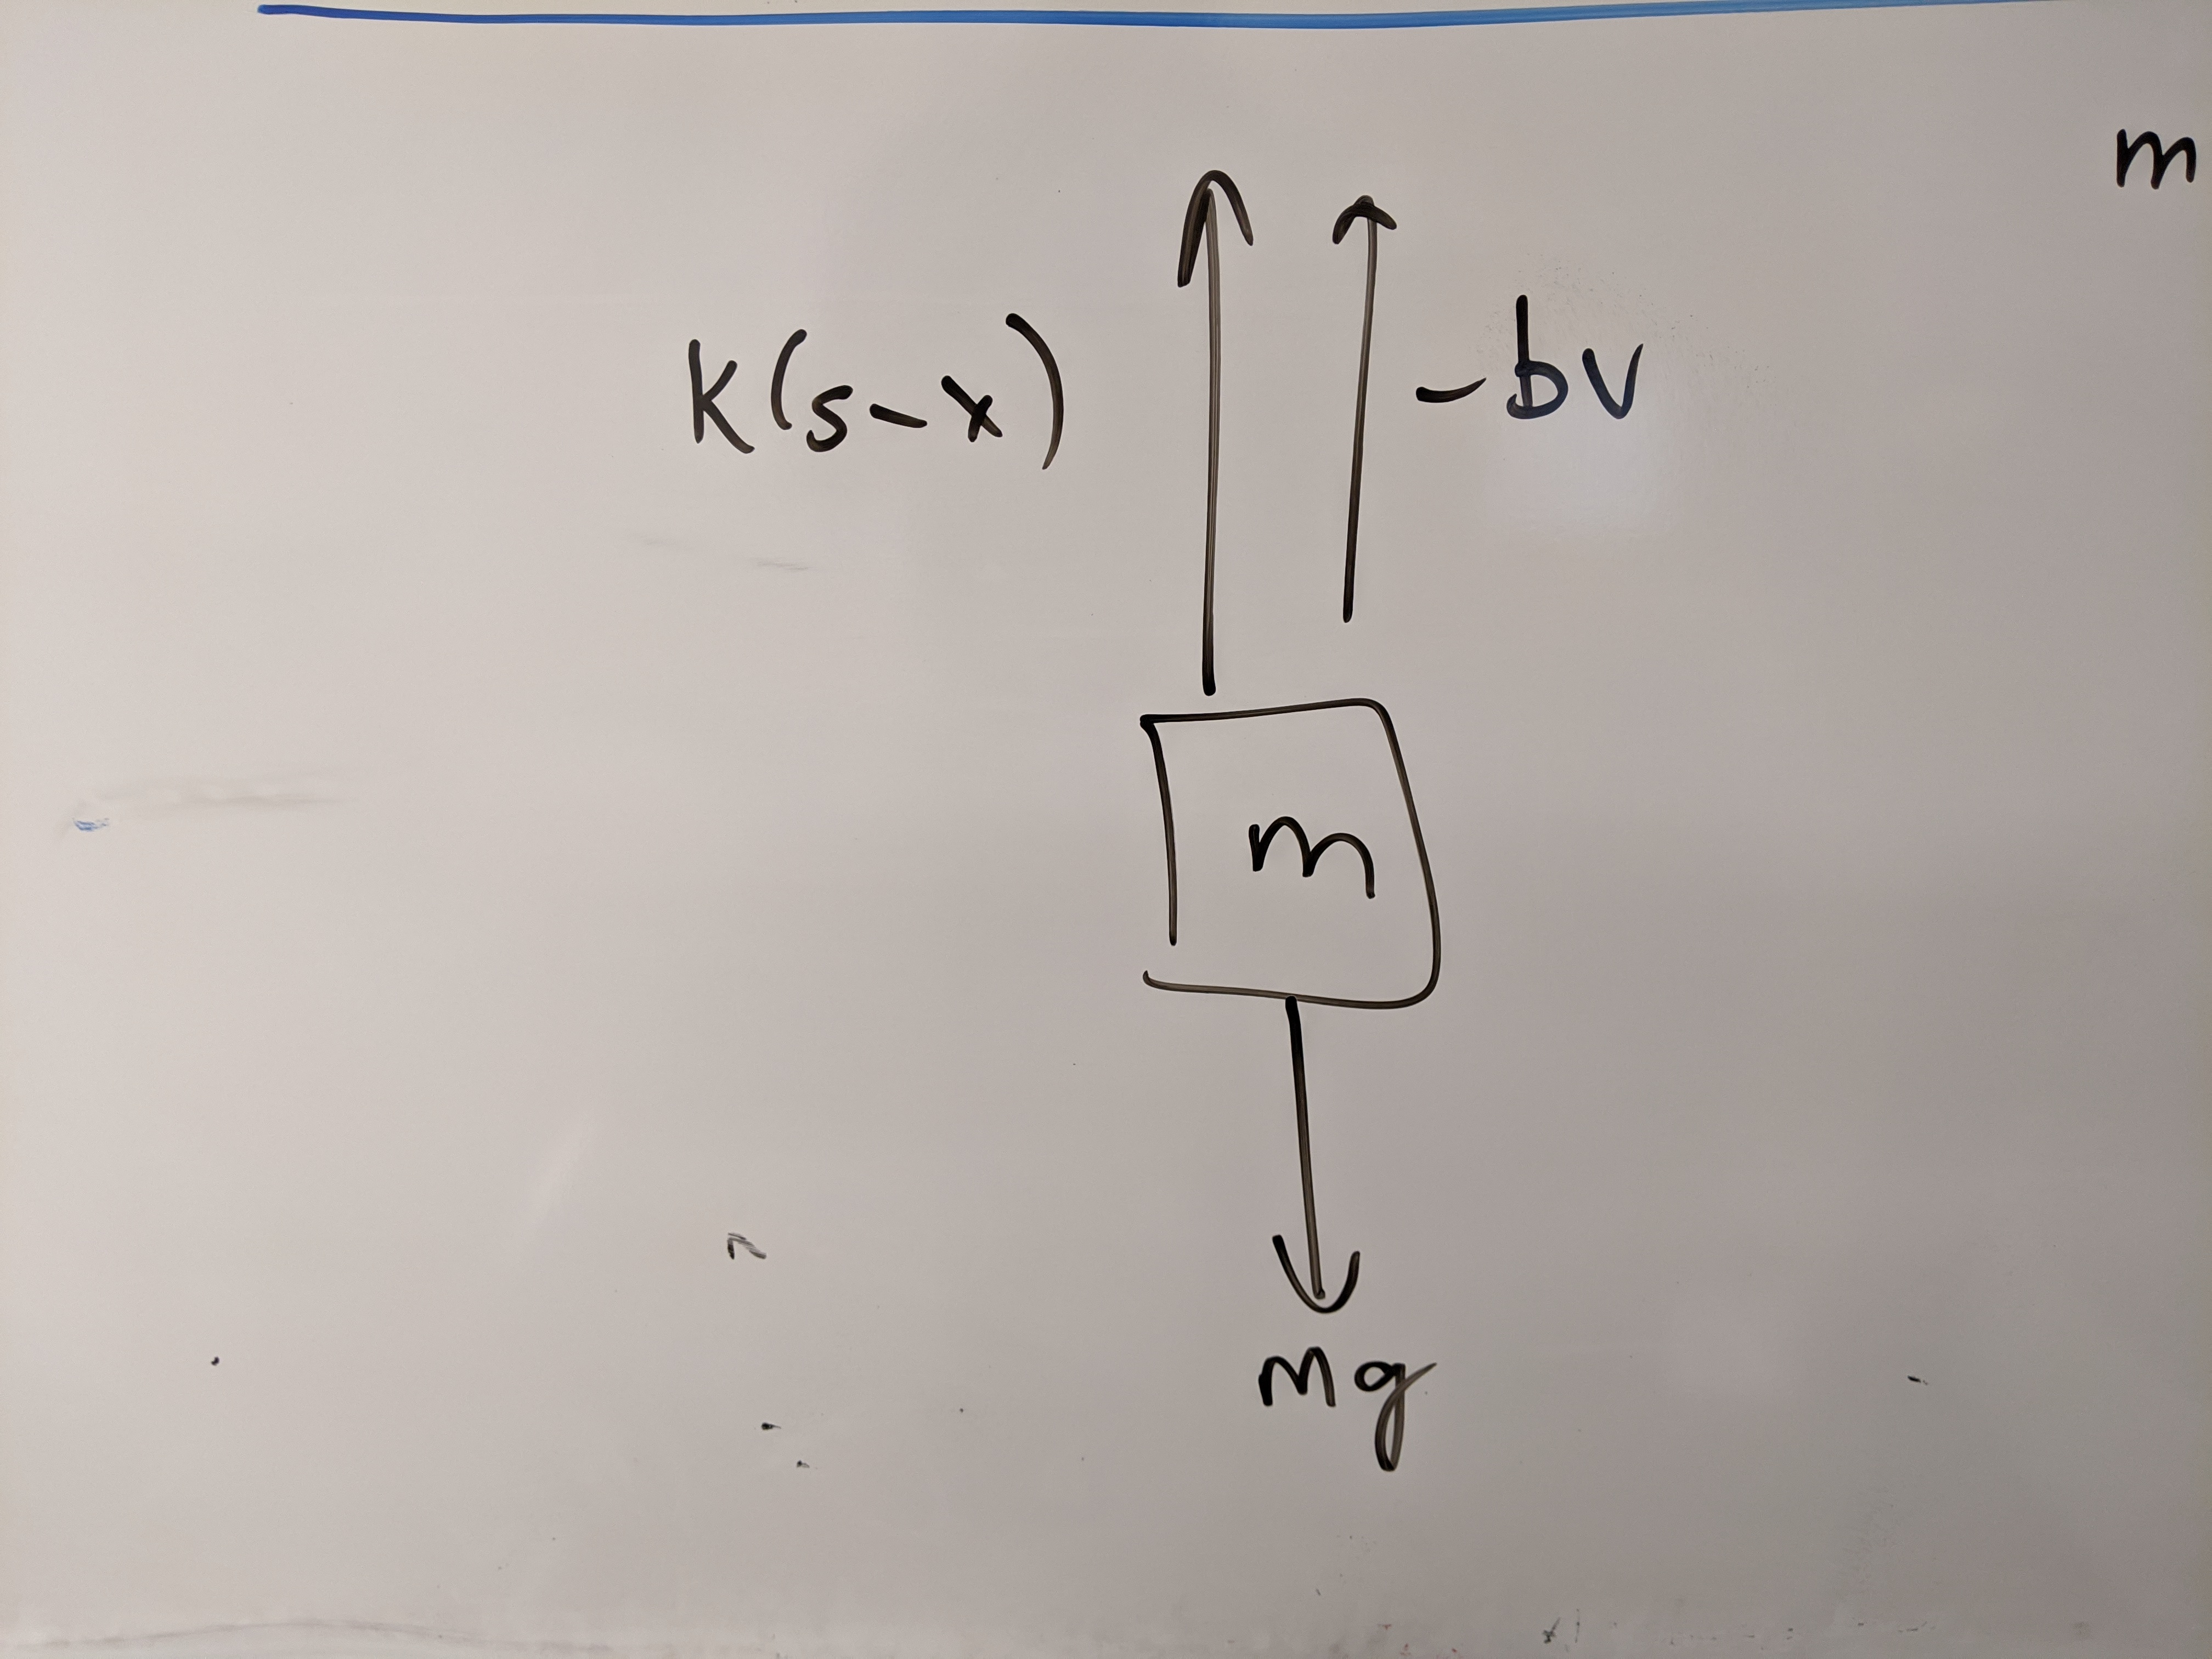
\includegraphics[width=\linewidth]{images/damped2.jpg}
\end{image}%
\begin{image}{0}{1}{0}%
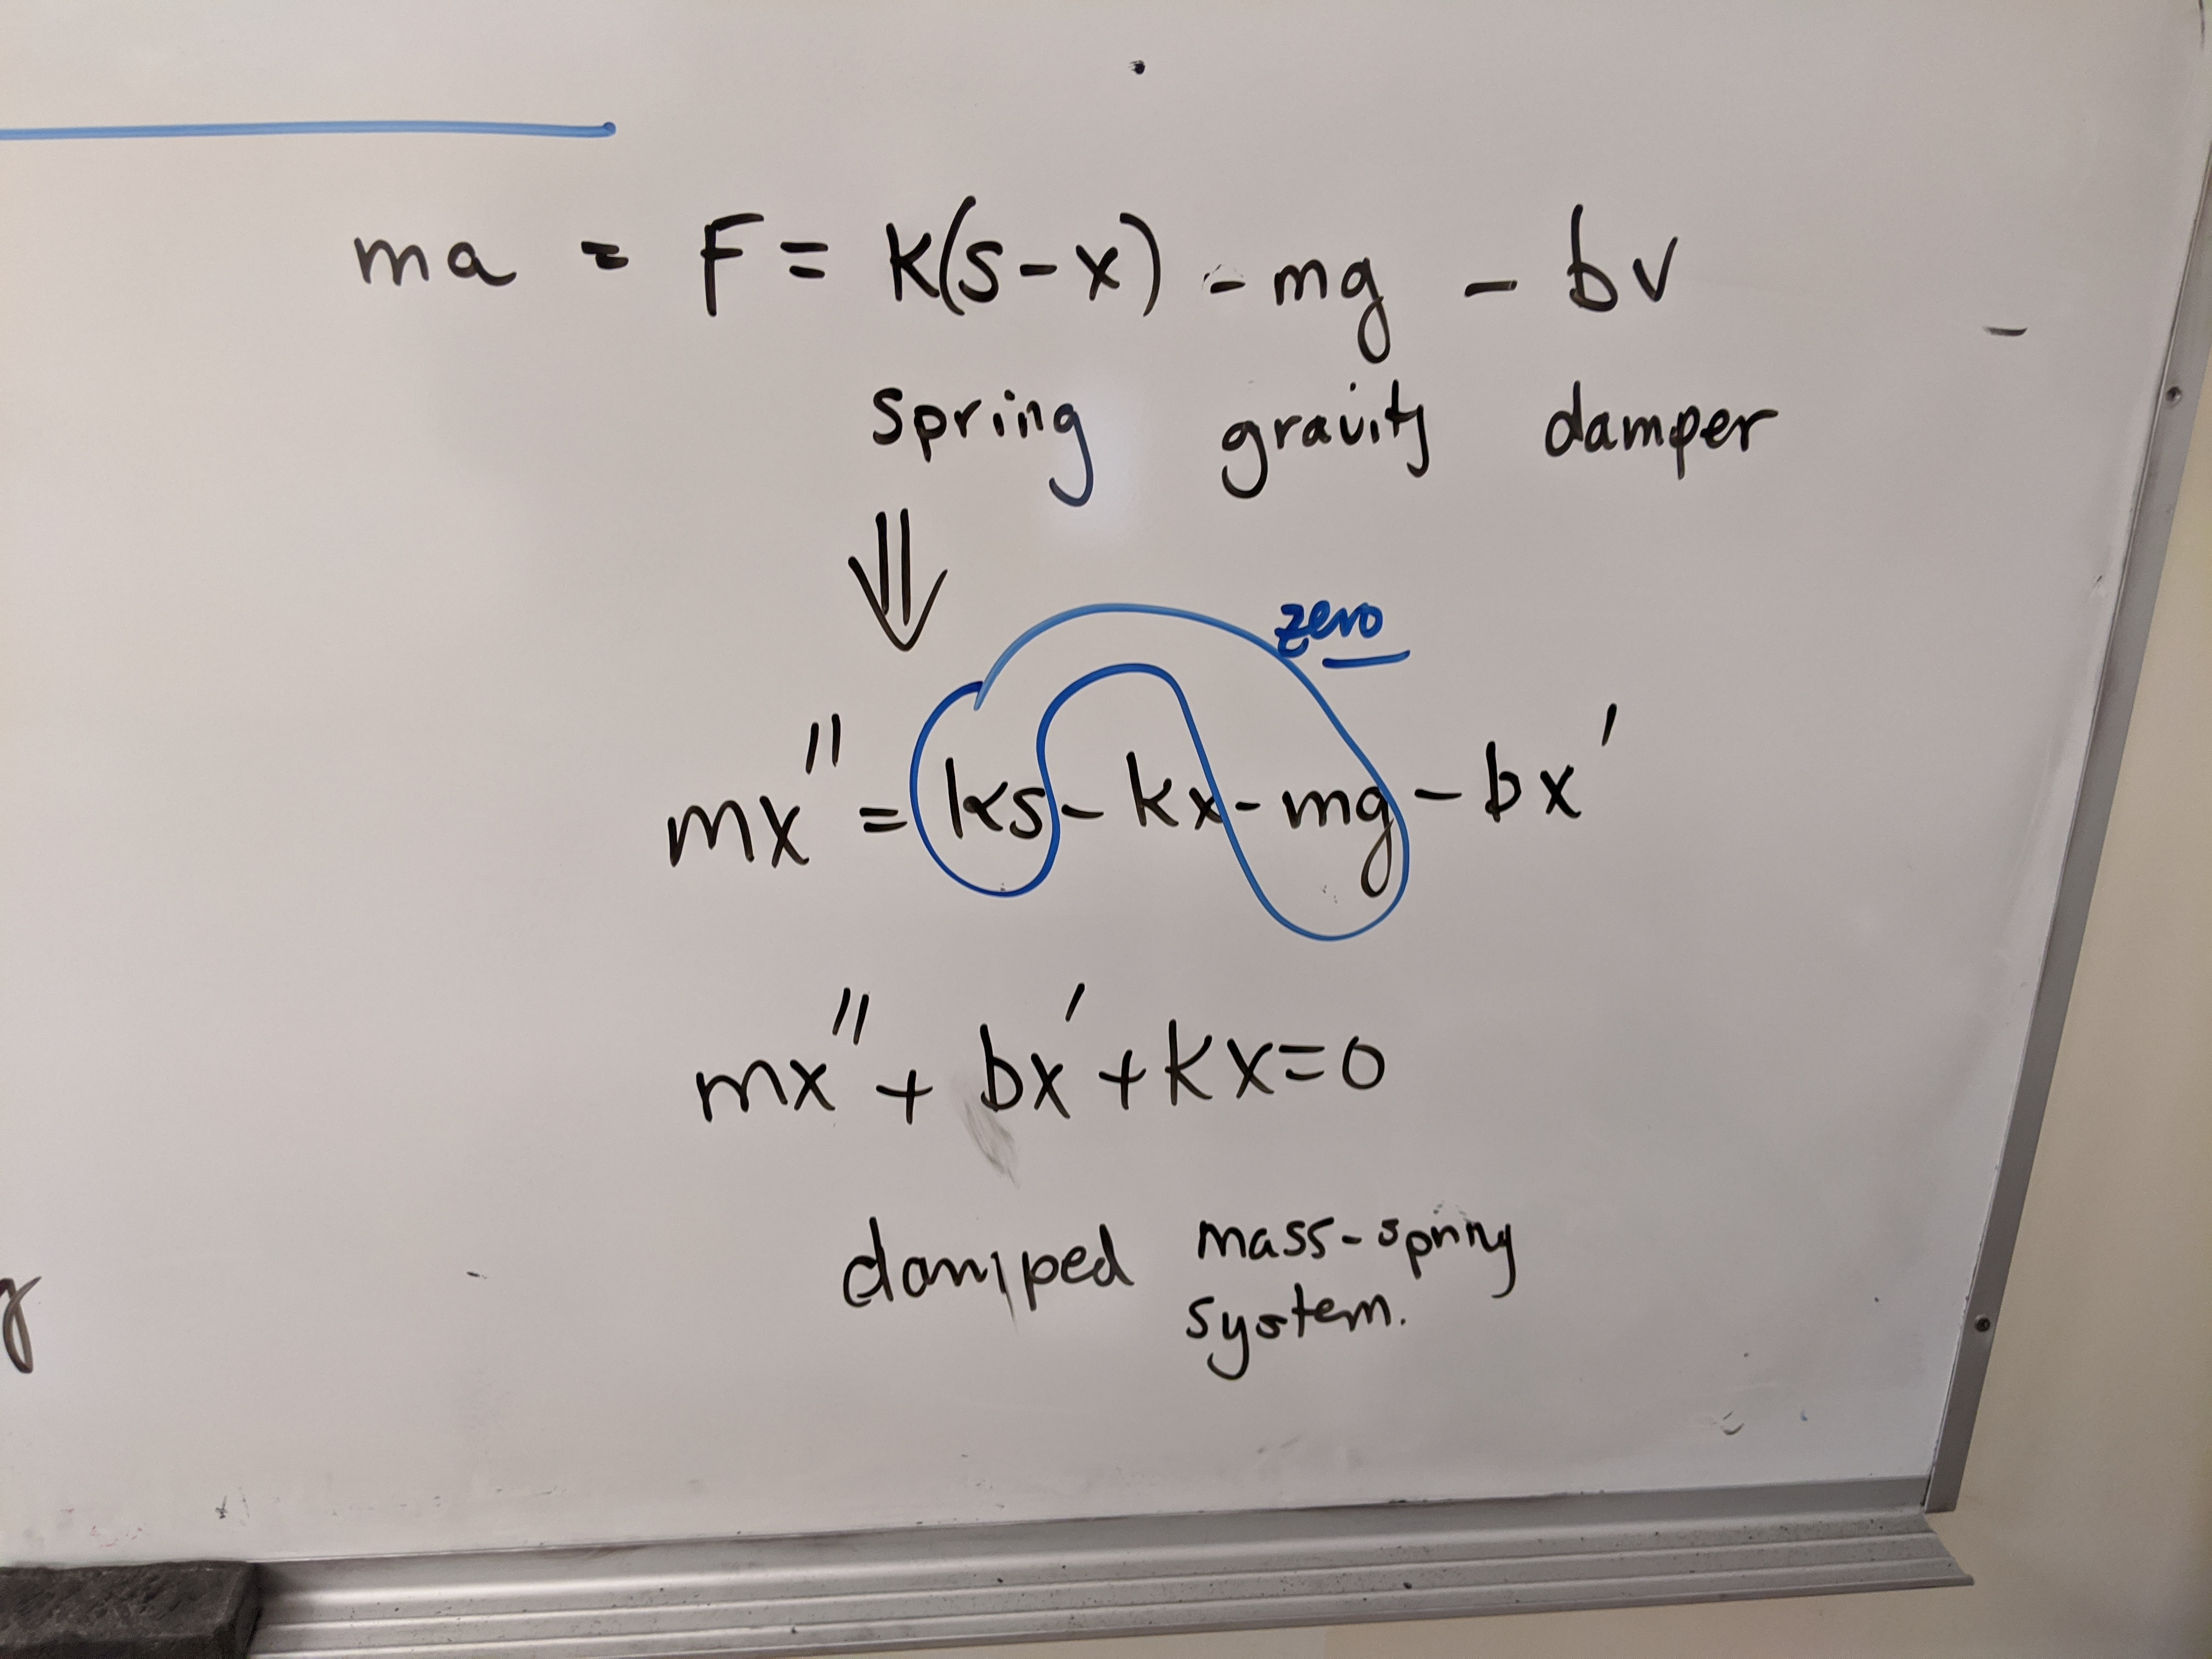
\includegraphics[width=\linewidth]{images/damped3.jpg}
\end{image}%
Thus, the equation for a damped mass-spring system is%
\begin{equation*}
x'' + \frac{b}{m} x' + \frac{k}{m} x = 0
\end{equation*}
which is also a second order linear equation with constant coefficients.%
\par
The mass-spring system is one of the most useful models in all of science. For example, RLC circuits (resistor\slash{}inductor\slash{}capacitor) are typically modeled as mass-spring systems.%
\par
This motivates the study of second order linear differential equations with constant coefficients, even though that might seem like an extremely restricted family of problems to think about. In later sections, we will extend our ideas to consider what happens if an external \emph{driving} or \emph{forcing function} is applied to the system.%
\par
We should already have an idea about the sorts of functions that solve these systems.%
\begin{enumerate}
\item{}Physical intuition tells us that when we release a mass attached to a spring from a non-equilibrium starting position, the mass oscillates up and down around the equilibrium position. This suggests that sine or cosine waves might be involved in the solution.%
\item{}Mathematical intuition tells us that functions that are related to their second derivatives by constant factors are also sines and cosines. That is, \((\sin x)'' = - \sin x\).%
\end{enumerate}
We will see that, indeed, this intuition is correct for undamped systems with no external forces.%
\end{subsectionptx}
\end{sectionptx}
%
%
\typeout{************************************************}
\typeout{Section 3.2 Second order linear equations}
\typeout{************************************************}
%
\begin{sectionptx}{Second order linear equations}{}{Second order linear equations}{}{}{x:section:ch3-2}
\begin{introduction}{}%
A \terminology{general second order ODE} is of the form%
\begin{equation*}
\frac{d^{2}y}{dt^{2}}=f\left(t,y,\frac{dy}{dt}\right).
\end{equation*}
As is the case with first order equations, we can describe a more structured family of equations. A \terminology{\(2^{nd}\) order linear ODE} is of the form%
\begin{equation*}
a(t)y^{\prime\prime}+b(t)y^{\prime}+c(t)y=d(t)
\end{equation*}
which can be rewritten as%
\begin{equation*}
y^{\prime\prime}+p(t)y^{\prime}+q(t)y=g(t).
\end{equation*}
A 2nd order ODE is called \terminology{homogeneous} if%
\begin{equation*}
a(t)y^{\prime\prime}+b(t)y^{\prime}+c(t)y=0
\end{equation*}
and \terminology{nonhomogeneous} if%
\begin{equation*}
a(t)y^{\prime\prime}+b(t)y^{\prime}+c(t)y=d(t)
\end{equation*}
for some \(d(t)\) that is NOT identically zero.%
\par
An intial value problem for a second order ODE needs to have \alert{two} initial conditions:%
\begin{align*}
y(t_{0}) \amp =y_{0},\\
y^{\prime}(t_{0}) \amp =y_{0}^{\prime}.
\end{align*}
%
\end{introduction}%
%
%
\typeout{************************************************}
\typeout{Subsection 3.2.1 Second order linear homogeneous ODEs with constant coefficients (characteristic equation)}
\typeout{************************************************}
%
\begin{subsectionptx}{Second order linear homogeneous ODEs with constant coefficients (characteristic equation)}{}{Second order linear homogeneous ODEs with constant coefficients (characteristic equation)}{}{}{g:subsection:idm45282413060032}
We will begin with the \terminology{2nd order linear homogeneous ODEs with constant coefficients} that we introduced and motivated in the previous section:%
\begin{equation*}
ay''+by^{\prime}+cy=0
\end{equation*}
where \(a,b,c\) are real constants.%
\par
Consider \(y^{\prime\prime}-y=0\) or%
\begin{equation*}
y^{\prime\prime}=y.
\end{equation*}
Can we think of a solution to this ODE from Calculus 1? A function where its second derivative is equal to itself?%
\par
A moment of thought should lead us to conclude that there are two obvious solutions: \(y_{1}(t)=e^{t}\) and \(y_{2}(t)=e^{-t}\). But it not hard to check that the larger family of functions \(y = c_{1}e^{t}\) and \(y = c_{2}e^{-t}\) are also solutions for any constants \(c_1, c_2\).%
\par
Now consider the general ODE%
\begin{equation*}
ay^{\prime\prime}+by^{\prime}+cy=0.
\end{equation*}
%
\par
Guided by our observation about the solutions to the previous equation, let us assume solutions are of the form \(y(t)=e^{rt}\). (If this is an unsatisfying assumption, another appoach will be explained shortly).  Then%
\begin{align*}
y(t) \amp =e^{rt}\\
y^{\prime}(t) \amp =re^{rt}\\
y^{\prime\prime}(t) \amp =r^{2}e^{rt},
\end{align*}
and plugging this into the ODE we have%
\begin{align*}
LHS=ar^{2}e^{rt}+bre^{rt}+ce^{rt} \amp \overset{?}{=}0\\
e^{rt}\left(ar^{2}+br+c\right) \amp \overset{?}{=}0.
\end{align*}
and since \(e^{rt}\neq0\) then%
\begin{equation*}
ar^{2}+br+c=0.
\end{equation*}
Using standard methods for quadratic equations, we can solve for the roots \(r=r_{1},r_{2}\).%
\par
This is called the \terminology{characteristic equation} of this ODE. If the roots \(r_1, r_2\) are \emph{real and distinct}, then the \terminology{general solution to the homogeneous equation} is of the form%
\begin{equation*}
y(t)=c_{1}e^{r_{1}t}+c_{2}e^{r_{2}t}.
\end{equation*}
%
\par
The justification for gluing together the solutions will be presented in the next section as the ``principle of superposition''.%
\begin{example}{}{g:example:idm45282412787984}%
Let's find the general solution of%
\begin{equation*}
y^{\prime\prime}+5y^{\prime}+6y=0.
\end{equation*}
%
%
\begin{enumerate}
\item{}We'll guess that the solution to a solution is \(y(t)=e^{rt}\) for some \(r\). Then get%
\begin{equation*}
\left(r^{2}+5r+6\right)e^{rt}=0
\end{equation*}
so that we must have \(r^{2}+5r+6=\left(r+2\right)\left(r+3\right)=0\) so that \(r=-2,-3\).%
\item{}So \(y_{1}(t)=e^{-2t}\) and \(y_{2}(t)=e^{-3t}\) are solutions and%
\begin{equation*}
y(t)=c_{1}e^{-2t}+c_{2}e^{-3t}
\end{equation*}
is the general solution.%
\end{enumerate}
\end{example}
\begin{example}{}{g:example:idm45282412781616}%
Let's find the solution to the following IVP%
\begin{equation*}
y^{\prime\prime}+5y^{\prime}+6y=0\,\,\,\,y(0)=2,y^{\prime}(0)=-1.
\end{equation*}
%
\par
Solving for the particular solution. We have \(y(0)=2\) and \(y^{\prime}(0)=-1\). Differentiating \(y(t)=c_{1}e^{-2t}+c_{2}e^{-3t}\) we get \(y^{\prime}(t)=-2c_{1}e^{-2t}-3c_{2}e^{-3t}\) and set up the following system:%
\begin{align*}
c_{1}+c_{2} \amp = \amp 2\\
-2c_{1}-3c_{2} \amp = \amp -1
\end{align*}
and get \(c_{1}=5,c_{2}=-3\). So the particular solution is%
\begin{equation*}
y(t)=5e^{-2t}-3e^{-3t}.
\end{equation*}
%
\end{example}
\begin{example}{}{g:example:idm45282412775792}%
Let's find the general solution of%
\begin{equation*}
2\frac{d^{2}y}{dt^{2}}+7\frac{dy}{dt}-4y=0.
\end{equation*}
%
%
\begin{enumerate}
\item{}We'll guess that the solution to a solution is \(y(t)=e^{rt}\) for some \(r\). Then get%
\begin{equation*}
\left(2r^{2}+7r-4\right)e^{rt}=0
\end{equation*}
so that we must have \(2r^{2}+7r-4=\left(2r-1\right)\left(r+4\right)=0\) so that \(r=\frac{1}{2},-4\).%
\item{}So \(y_{1}(t)=e^{t/2}\) and \(y_{2}(t)=e^{-4t}\) are solutions and%
\begin{equation*}
y(t)=c_{1}e^{t/2}+c_{2}e^{-4t}
\end{equation*}
is the general solution.%
\end{enumerate}
\end{example}
\end{subsectionptx}
%
%
\typeout{************************************************}
\typeout{Subsection 3.2.2 Derivatives as linear operators and the characteristic equation}
\typeout{************************************************}
%
\begin{subsectionptx}{Derivatives as linear operators and the characteristic equation}{}{Derivatives as linear operators and the characteristic equation}{}{}{g:subsection:idm45282412769264}
It might seem unsatisfying to assume the form of an answer and then show that our guess worked. Is there a mathematical justification for making this guess? The answer is yes, if we're willing to push our understanding of differentiation slightly.%
\par
Define the \terminology{differential operator} \(D\) to be the operation of applying \(\frac{d}{dx}\) to a function \(y(x)\). The operator \(D\) can be thought of as a function on functions:%
\begin{equation*}
D(\text{function}) = \text{ derivative}.
\end{equation*}
Any order of derivative can be thought of this way. For example,%
\begin{equation*}
y''' = \frac{d^3 y}{dx^3} = \frac{d^3}{dx^3} y = D^3 y.
\end{equation*}
We need a notion of \(D^0\) - what should that mean? It makes sense to set \(D^0(y) = y\) - that is, take no derivatives of \(y\). We will use the symbol \(1\) to represent this function, the \terminology{identity function} that leaves \(y\) unchanged.%
\par
In Calculus, we learn that derivatives follow certain rules. Two of the most important are%
\begin{equation*}
D(f + g) = Df + Dg
\end{equation*}
and%
\begin{equation*}
D(cf) = cD(f).
\end{equation*}
These two properties together show that \(D\) is a \terminology{linear function}.%
\par
Using differential operator notation allows us to transform an ODE and use algebraic techniques to solve it using first order methods. Consider the equation%
\begin{equation*}
y'' + 3 y ' + 2 y = 0.
\end{equation*}
This can be written%
\begin{equation*}
D^2 y + 3 D y + 2 y = 0
\end{equation*}
using operator notation. But since each operator is applied to the same input, \(y\), we can use function notation to write%
\begin{equation*}
(D^2 + 3D + 2)(y) = 0.
\end{equation*}
%
\par
The operator expression \(D^2 + 3D + 2\) can be factored as symbols into \((D + 2)(D + 1)\) (that this is equal to the original equation applied to \(y\) is a consequence of linearity). Now, using the fact that the derivative of 0 is 0, we assert that the solutions to the equation%
\begin{equation*}
(D + 1)(D + 2)y = (D + 2)(D+1)y = 0
\end{equation*}
are the solutions to \((D + 1)(y) = 0\) and \((D + 2)y = 0\), which are just the first order equations%
\begin{gather*}
y' + y = 0\\
y' + 2y = 0
\end{gather*}
These are separable, with solutions \(y_1 = c_1 e^{-x}\) and \(y_2 = c_2 e^{-2x}\). So the general solution (justified by the principle of superposition, covered in the next section) to the ODE is%
\begin{equation*}
y = c_1 e^{-x} + c_2 e^{-2x}.
\end{equation*}
%
\par
Note that the operator polynomial \(D^2 + 3D + 2\) is precisely equivalent to the characteristic polynomial \(r^2 + 3r + 2\).%
\end{subsectionptx}
\end{sectionptx}
%
%
\typeout{************************************************}
\typeout{Section 3.3 Solutions to Linear Equations; the Wronskian}
\typeout{************************************************}
%
\begin{sectionptx}{Solutions to Linear Equations; the Wronskian}{}{Solutions to Linear Equations; the Wronskian}{}{}{x:section:ch3-3}
\begin{introduction}{}%
In this section, we will consider equations of the form%
\begin{equation*}
y^{\prime\prime}+p(t)y^{\prime}+q(t)y=0,\,\,\,\,\,y(t_{0})=y_{0},\,\,\,\,y^{\prime}(t_{0})=y_{0}^{\prime}.
\end{equation*}
where \(a,b,c\) are constants. This is a second order, linear, homogeneous equation. Our goal is to find the general solution of these equations.%
\begin{theorem}{(Existence and Uniqueness for \(2\)nd order linear ODES).}{}{x:theorem:thm2ndexist}%
Consider the IVP%
\begin{equation*}
y^{\prime\prime}+p(t)y^{\prime}+q(t)y=g(t),\,\,\,\,\,y(t_{0})=y_{0},\,\,\,\,y^{\prime}(t_{0})=y_{0}^{\prime}
\end{equation*}
where \(p,q,g\) are continuous on an open interval \(I\) that contains \(t_{0}\). Then there exists a unique solution \(y=\phi(t)\), and the solution exists throughout all of \(I\).%
\end{theorem}
Recall that this theorem implies that a solution to this IVP%
\begin{enumerate}
\item{}exists,%
\item{}is unique%
\item{}and the solution \(\phi\) is defined throughout all of \(I\).%
\end{enumerate}
In fact it says more, namely that \(\phi\) is at least twice differentiable on \(I\).%
\begin{example}{}{g:example:idm45282413018880}%
Find the longest interval in which the solution to the IVP is certain to exist by \hyperref[x:theorem:thm2ndexist]{Theorem~\ref{x:theorem:thm2ndexist}}:%
\begin{equation*}
\left(t^{4}-4t^{2}\right)y^{\prime\prime}+\cos ty^{\prime}-e^{t}y=0,\,\,\,\,\,\,y(1)=2,\,\,\,y^{\prime}(1)=1.
\end{equation*}
%
\par
\alert{Solution:} Rewrite the equation as%
\begin{equation*}
y^{\prime\prime}+\frac{\cos t}{t^{2}\left(t^{2}-4\right)}y^{\prime}-\frac{e^{t}}{t^{2}\left(t^{2}-4\right)}y=0.
\end{equation*}
so that \(p(t)=\frac{\cos t}{t^{2}\left(t^{2}-4\right)}\) and \(q(t)=-\frac{e^{t}}{t^{2}\left(t^{2}-4\right)}\) which are both continuous on \(\left(-\infty,-2\right)\cup\left(-2,0\right)\cup\left(0,2\right)\cup\left(2,\infty\right)\). Since \(t_{0}=1\in\left(0,2\right)\) then \(I=\left(0,2\right)\) is the longest interval where \(p(t)\) and \(q(t)\) are both continuous that contains \(t_{0}\).%
\end{example}
\end{introduction}%
%
%
\typeout{************************************************}
\typeout{Subsection 3.3.1 Principle of Superposition}
\typeout{************************************************}
%
\begin{subsectionptx}{Principle of Superposition}{}{Principle of Superposition}{}{}{g:subsection:idm45282413011632}
We now give a name to idea that linear combinations of solutions to a linear homogeneous differential equation remain solutions. (Again, the underlying principle is the linearity of the differential operator.)%
\begin{theorem}{Superposition of solutions to linear homogeneous ODE.}{}{g:theorem:idm45282413010240}%
If \(y_{1}\) and \(y_{2}\) are two solutions to an ODE%
\begin{equation*}
y^{\prime\prime}+p(t)y^{\prime}+q(t)y=0,
\end{equation*}
then the linear combination \(y(t)=c_{1}y_{1}(t)+c_{2}y_{2}(t)\) is also a solution for any values \(c_{1},c_{2}\).%
\end{theorem}
\alert{Warning:} The principle of superposition holds only if the equation is \emph{linear} and \emph{homogeneous}.%
\begin{example}{}{g:example:idm45282413004976}%
Suppose \(y_{1}(t)=e^{-t}\) and \(y_{2}(t)=e^{t}\) are two solutions to \(y^{\prime\prime}-y=0\). Since this is a linear homogeneous ODE then the principle of superposition says that the function%
\begin{equation*}
y(t)=2e^{-t}+3e^{t}
\end{equation*}
is also a solution.%
\end{example}
\begin{example}{}{g:example:idm45282412673632}%
It is not hard to check that \(y_{1}(t)=1\) and \(y_{2}(t)=t^{\frac{1}{2}}\) are solutions to%
\begin{equation*}
yy^{\prime\prime}+\left(y^{\prime}\right)^{2}=0,\,\,\,t>0.
\end{equation*}
%
\par
Part (a): Show \(y(t)=1+2t^{\frac{1}{2}}\) is not a solution to this ODE:%
\par
Solution: First compute%
\begin{align*}
y(t) \amp =1+2t^{\frac{1}{2}}\\
y^{\prime}(t) \amp =t^{-\frac{1}{2}}\\
y^{\prime\prime}(t) \amp =-\frac{1}{2}t^{-\frac{3}{2}}
\end{align*}
To show this simply check if the LHS equal to \(0\):%
\begin{align*}
LHS \amp =yy^{\prime\prime}+\left(y^{\prime}\right)^{2}=\left(1+2t^{\frac{1}{2}}\right)\left(-\frac{1}{2t^{3/2}}\right)+\left(\frac{1}{t^{\frac{1}{2}}}\right)^{2}\\
\amp =-\frac{1}{2t^{3/2}}-\frac{1}{t}+\frac{1}{t}=-\frac{1}{2t^{3/2}}\neq0,
\end{align*}
%
\par
Part (b): Why does this not contradict the Principle of Superposition?%
\par
Solution: To apply the principle, the equation needs to be linear. The term \(\left(y^{\prime}\right)^{2}\) in the ODE makes this nonlinear, hence we can't even use the principle in the first place.%
\end{example}
\end{subsectionptx}
%
%
\typeout{************************************************}
\typeout{Subsection 3.3.2 Fundamental sets of solutions}
\typeout{************************************************}
%
\begin{subsectionptx}{Fundamental sets of solutions}{}{Fundamental sets of solutions}{}{}{g:subsection:idm45282412664512}
Suppose that \(y_{1}(t)\) and \(y_{2}(t)\) are two solutions to a second order linear homogeneous equation. When do we know that%
\begin{equation*}
y(t)=c_{1}y_{1}(t)+c_{2}y_{2}(t)
\end{equation*}
is the \terminology{general solution} to the ODE? That is, when do we know that we can obtain \emph{every single solution} to an IVP? To answer that we need to define some machinery.%
\begin{definition}{}{g:definition:idm45282412660864}%
The determinant of a matrix \(\left(\begin{array}{cc}
a \amp b\\
c \amp d
\end{array}\right)\) is%
\begin{equation*}
\left|\begin{array}{cc}
a \amp b\\
c \amp d
\end{array}\right|=ad-bc.
\end{equation*}
\end{definition}
\begin{definition}{}{g:definition:idm45282412659344}%
The \terminology{Wronskian} of the solutions \(y_{1}(t)\) and \(y_{2}(t)\) to a second order linear homogeneous ODE is the function%
\begin{equation*}
W=W(y_{1},y_{2})(t)=\left|\begin{array}{cc}
y_{1}(t) \amp y_{2}(t)\\
y_{1}^{\prime}(t) \amp y_{2}^{\prime}(t)
\end{array}\right|.
\end{equation*}
\end{definition}
The Wronskian computes a function that can be used to check of a solution set is sufficient to construct every possible solution.%
\begin{theorem}{General solution theorem.}{}{x:theorem:thmgensol}%
Suppose \(y_{1}\) and \(y_{2}\) are two solutions to the ODE%
\begin{equation*}
y^{\prime\prime}+p(t)y^{\prime}+q(t)y=0
\end{equation*}
in some interval \(I\) where \(p,q\) are continuous. Then the family of solutions%
\begin{equation*}
y(t)=c_{1}y_{1}(t)+c_{2}y_{2}(t)
\end{equation*}
for arbtitrary \(c_{1},c_{2}\) is the general solution if and only if the Wronskian \(W\left(y_{1},y_{2}\right)\) is not zero for at least one point \(t_{0}\) in \(I\).%
\end{theorem}
\begin{example}{}{g:example:idm45282412649824}%
Find the general solution to%
\begin{equation*}
y^{\prime\prime}+4y^{\prime}-5y=0.
\end{equation*}
%
\par
Solution: In the last section we showed that to find solutions to this ODE we simply need to solve the characteristic equation%
\begin{equation*}
r^{2}+4r-5=\left(r-1\right)\left(r+5\right)=0
\end{equation*}
and get \(r=1,-5\) so that%
\begin{equation*}
y(t)=c_{1}e^{t}+c_{2}e^{-5t}
\end{equation*}
gives other solutions to the ODE. To show this gives all of them, we simply need to show the Wronksian is not always zero:%
\begin{align*}
W\left(e^{t},e^{-5t}\right) \amp =\left|\begin{array}{cc}
y_{1}(t) \amp y_{2}(t)\\
y_{1}^{\prime}(t) \amp y_{2}^{\prime}(t)
\end{array}\right|=\left|\begin{array}{cc}
e^{t} \amp e^{-5t}\\
e^{t} \amp -5e^{-5t}
\end{array}\right|\\
\amp =-5e^{-4t}-e^{-4t}\\
\amp =-6e^{-4t}\\
\amp \neq0.
\end{align*}
%
\end{example}
To find the general solution of \(y^{\prime\prime}+p(t)y^{\prime}+q(t)y=g(t)\), we only need to find two (\(y_{1},y_{2}\)) solutions whose Wronskian is nonzero:%
\begin{enumerate}
\item{}First find two solutions \(y_{1},y_{2}\).%
\item{}Then check \(W(y_{1},y_{2})\neq0\) for at least one point in the interval.%
\end{enumerate}
%
\begin{definition}{}{g:definition:idm45282412640480}%
The solutions \(y_{1}\) and \(y_{2}\) are said to form a \terminology{fundamental set of solutions} to%
\begin{equation*}
y^{\prime\prime}+p(t)y^{\prime}+q(t)y=0
\end{equation*}
if \(W\left(y_{1},y_{2}\right)\neq0\).%
\end{definition}
\begin{example}{}{g:example:idm45282412637232}%
Verify that \(y_{1}(t)=t^{\frac{1}{2}}\) and \(y_{2}(t)=t^{-1}\) form a fundamental set of solutions of%
\begin{equation*}
2t^{2}y^{\prime\prime}+3ty^{\prime}-y=0,\,\,\,\,\,t>0.
\end{equation*}
%
\par
Solution:%
\par
Part (a): First we verify these are indeed solutions by plugging them into the LHS and checking that they equal zero. First computer some derivatives%
\begin{equation*}
\begin{array}{ccc}
y_{1}(t)=t^{\frac{1}{2}} \amp  \amp y_{2}(t)=t^{-1}\\
y_{2}^{\prime}(t)=\frac{1}{2}t^{-\frac{1}{2}} \amp  \amp y_{2}^{\prime}(t)=-t^{-2}\\
y_{3}^{\prime}(t)=-\frac{1}{4}t^{-\frac{3}{2}} \amp  \amp y_{2}^{\prime\prime}(t)=-t^{-2}.
\end{array}
\end{equation*}
Plugging \(y_{1}\) into LHS we get%
\begin{align*}
LHS \amp =2t^{2}y_{1}^{\prime\prime}+3ty_{1}^{\prime}-y_{1}\\
\amp =2t^{2}\left(-\frac{1}{4}t^{-\frac{3}{2}}\right)+3t\left(\frac{1}{2}t^{-\frac{1}{2}}\right)-\left(t^{\frac{1}{2}}\right)\\
\amp =-\frac{1}{2}t^{\frac{1}{2}}+\frac{3}{2}t^{\frac{1}{2}}-t^{\frac{1}{2}}\\
\amp =0.
\end{align*}
Thus \(y_{1}\) is a solution. It is very similar to show \(y_{2}\) is a solution.%
\par
Part (b): To show \(y_{1}y_{2}\) form a fundamental set of solutions, we simply need to show that \(W(y_{1},y_{2})\) is nonzero:%
\begin{equation*}
W(y_{1},y_{2})=\left|\begin{array}{cc}
t^{\frac{1}{2}} \amp t^{-1}\\
\frac{1}{2}t^{-\frac{1}{2}} \amp -t^{-2}
\end{array}\right|=-\frac{3}{2}t^{-3/2}\neq0
\end{equation*}
which is nonzero for \(t>0\).%
\end{example}
\end{subsectionptx}
\end{sectionptx}
%
%
\typeout{************************************************}
\typeout{Section 3.4 Complex roots of the characteristic equation}
\typeout{************************************************}
%
\begin{sectionptx}{Complex roots of the characteristic equation}{}{Complex roots of the characteristic equation}{}{}{x:section:ch3-4}
%
%
\typeout{************************************************}
\typeout{Subsection 3.4.1 Complex numbers:}
\typeout{************************************************}
%
\begin{subsectionptx}{Complex numbers:}{}{Complex numbers:}{}{}{g:subsection:idm45282412625376}
Complex numbers are of the form \(z = a+bi\) where \(a,b\in\mathbb{R}\) and \(i=\sqrt{-1}\). Thus \(i^{2}=-1\). Complex numbers have a \terminology{polar representation} \(z = r e^{i\theta}\), where \(r = \sqrt{a^2 + b^2}\) and \(\theta = \arctan\frac{y}{x}\). In the polar representation, we should think about \(r\) as a radius and \(e^{i\theta}\) as a point on the unit circle.%
\par
We should think about the exponential part as representing motion on a circle. The unit circle from trigonometry gives \((x,y) = (\cos \theta, \sin \theta)\) for an angle \(\theta\) on the unit circle. This connection is made explicit in what is known as \terminology{Euler's formula:}%
\begin{equation*}
e^{i\theta}=\cos \theta+i\sin \theta.
\end{equation*}
So%
\begin{equation*}
e^{a+ib}=e^{a}e^{ib}=e^{a}\left(\cos b+i\sin b\right)=e^{a}\cos b+ie^{a}\sin b.
\end{equation*}
%
\end{subsectionptx}
%
%
\typeout{************************************************}
\typeout{Subsection 3.4.2 Complex roots to the characteristic equation}
\typeout{************************************************}
%
\begin{subsectionptx}{Complex roots to the characteristic equation}{}{Complex roots to the characteristic equation}{}{}{g:subsection:idm45282412719904}
Suppose we are solving the constant coefficient 2nd order linear differential equation%
\begin{equation*}
ay^{\prime\prime}+by^{\prime}+cy=0.
\end{equation*}
and that solving the characteristic equation%
\begin{equation*}
ar^{2}+br+c=0
\end{equation*}
gives that the roots are%
\begin{equation*}
r_1=a + ib \text{ and }r_2=a - ib.
\end{equation*}
(Remember that complex roots of real polynomials always come in conjugate pairs.)%
\par
These roots are distinct, so we can apply the form of solutions we developed in the previous section. So for the root \(r_1 = a + ib\), the solution is of the form%
\begin{align*}
y(t) \amp =e^{r_1t}=e^{\left(a+ib \right)t}=e^{a t}e^{ib t}\\
\amp =e^{a t}\left(\cos\left(b t\right)+i\sin\left(b t\right)\right)\\
\amp =e^{a t}\cos\left(b t\right)+ie^{a t}\sin\left(b t\right)\\
\amp =u(t)+iv(t)
\end{align*}
where \(u(t)=e^{a t}\cos\left(b t\right)\) is the real part and \(v(t)=e^{a t}\sin\left(b t\right)\) is the imaginary part.%
\par
The complex form of the solution is frequently useful for computational purposes, but in practice (and for non-mathematicians) we prefer real solutions. Because the differential operator is linear, we have the following theorem:%
\begin{theorem}{}{}{g:theorem:idm45282412712128}%
If \(y(t)=u(t)+iv(t)\) is a complex solution to an ODE of the form \(ay^{\prime\prime}+by^{\prime}+cy=0\), then so are \(u(t)\) and \(v(t)\).%
\end{theorem}
Therefore since \(u(t)=e^{a t}\cos\left(b t\right)\) and \(v(t)=e^{a t}\sin\left(b t\right)\) are solutions we can compute (after some tedious work) that the Wronskian of \(u\) and \(v\) are:%
\begin{equation*}
W\left(u,v\right)(t)=\mu e^{2a t}\neq0\text{ as long as }b\neq0.
\end{equation*}
Hence by the \hyperref[x:theorem:thmgensol]{Theorem~\ref{x:theorem:thmgensol}}, because the Wronskian is not zero we have that \(u(t)\) and \(v(t)\) form a fundamental set of solutions. In other words, the general solution to \(a y '' + by' + cy = 0\) is%
\begin{equation*}
y_g = e^{at} (c_1 \cos(bt) + c_2\sin(bt)).
\end{equation*}
%
\end{subsectionptx}
%
%
\typeout{************************************************}
\typeout{Subsection 3.4.3 Examples}
\typeout{************************************************}
%
\begin{subsectionptx}{Examples}{}{Examples}{}{}{g:subsection:idm45282412704048}
So far, we can solve two cases of second order linear constant coefficient homogeneous differential equations. For%
\begin{equation*}
a\frac{d^{2}y}{dt^{2}}+b\frac{dy}{dt}+cy=0
\end{equation*}
and roots \(r_1, r_2\) of%
\begin{equation*}
ar^{2}+br+c=0,
\end{equation*}
the general solutions are the following:%
\begin{equation*}
\begin{array}{|c|c|c|}
\hline
\text{Roots} \amp \text{General solution} \amp \text{Example}\\
\hline
r_{1},r_{2}= \text{real, distinct} \amp y(t)=c_{1}e^{r_{1}t}+c_{2}e^{r_{2}t} \amp \left(r+1\right)\left(r-1\right)=r^{2}-1=0\\
\hline
r=a \pm ib, \text{imaginary} \amp y(t)=c_{1}e^{a t}\cos b t+c_{2}e^{a t}\sin b t \amp r^{2}+1=0\\
\hline
\end{array}
\end{equation*}
%
\begin{example}{}{g:example:idm45282412700624}%
Let's find the general solution of%
\begin{equation*}
\frac{d^{2}y}{dt}+4\frac{dy}{dt}+13y=0
\end{equation*}
%
\par
Step 1: We can jump straight to the characteristic equation:%
\begin{equation*}
r^{2}+4r+13=0,
\end{equation*}
which we can solve this using the quadratic formula:%
\begin{equation*}
r=\frac{-4\pm\sqrt{16-4\cdot13}}{2}=-2\pm\frac{1}{2}\sqrt{4(4-13)}=-2\pm\sqrt{-9}=-2\pm3i.
\end{equation*}
(Or you can use a completing the square trick%
\par
Step 2: The general solution is%
\begin{equation*}
y(t)=c_{1}e^{-2t}\cos3t+c_{2}e^{-2t}\sin3t.
\end{equation*}
%
\end{example}
\begin{example}{}{g:example:idm45282412696784}%
Let's find the particular solution to the IVP:%
\begin{equation*}
y^{\prime\prime}+9y=0,\,\,\,\,\,\,y(0)=-2,\,\,\,y^{\prime}(0)=1
\end{equation*}
%
\par
Step 1: We can jump straight to the characteristic equation:%
\begin{equation*}
r^{2}+9=0
\end{equation*}
and get \(r=\pm3i\).%
\par
Step 2: The general solution is%
\begin{align*}
y(t) \amp =c_{1}e^{0t}\cos3t+c_{2}e^{0t}\sin3t.\\
\amp =c_{1}\cos3t+c_{2}\sin3t.
\end{align*}
%
\par
Step 3: Using the initial conditions \(y(0)=-2,\,\,\,y^{\prime}(0)=1\) we need to first take a derivative%
\begin{align*}
y(t) \amp =c_{1}\cos3t+c_{2}\sin3t\\
y^{\prime}(t) \amp =-3c_{1}\sin3t+3c_{2}\cos3t
\end{align*}
hence%
\begin{align*}
-2 \amp =y(0)=c_{1}+0\\
1 \amp =y^{\prime}(0)=0+3c_{2}
\end{align*}
so that%
\begin{equation*}
c_{1}=-2,c_{2}=\frac{1}{3}.
\end{equation*}
Thus the solution is%
\begin{equation*}
y(t)=-2\cos3t+\frac{1}{3}\sin3t.
\end{equation*}
%
\end{example}
\begin{example}{}{g:example:idm45282412687808}%
Suppose we get that the general solution comes out to%
\begin{equation*}
y(t)=c_{1}e^{3t}\cos t+c_{2}e^{3t}\sin t.
\end{equation*}
Then just remember when finding constants corresponding to initial conditions that we need to use product rule to find the derivative of \(y(t)\):%
\begin{equation*}
y^{\prime}(t)=3c_{1}e^{3t}\cos t-c_{1}e^{3t}\sin t+3c_{2}e^{3t}\sin t+c_{2}e^{3t}\cos t.
\end{equation*}
%
\end{example}
\end{subsectionptx}
\end{sectionptx}
%
%
\typeout{************************************************}
\typeout{Section 3.5 Repeated roots; Reduction of order}
\typeout{************************************************}
%
\begin{sectionptx}{Repeated roots; Reduction of order}{}{Repeated roots; Reduction of order}{}{}{x:section:ch3-5}
%
%
\typeout{************************************************}
\typeout{Subsection 3.5.1 Repeated roots}
\typeout{************************************************}
%
\begin{subsectionptx}{Repeated roots}{}{Repeated roots}{}{}{g:subsection:idm45282412683728}
Suppose that we are given the differential equation%
\begin{equation*}
ay'' + by' + cy = 0
\end{equation*}
and that \(b^2 - 4ac = 0\). Then the characteristic equation must have the form%
\begin{align*}
ar^2 + br + c \amp= ar^2 + br + \frac{b^2}{4a}\\
\amp= a(r + \frac{b}{2a})^2
\end{align*}
That is, the equation has just one root, \(r = -\frac{b}{2a}\). The results of the previous section say that the function \(y = e^{-\frac{b}{2a} t}\) is a solution to the equation. But this is just one solution. We can't use another copy of the function as a second solution because it isn't linearly independent from the first - we will not have a fundamental set, nor will we know the general equation.%
\par
So the question is how to get a second solution from only our knowledge of the first. Because the roots are repeated, we may well guess that some kind of modification of the first solution \(y_1 = e^{-\frac{b}{2a} t}\) will give us what we want, but we need to use more than a constant or again we'll fail to have a fundamental set. It seems reasonable to guess that the second solution should have the form%
\begin{equation*}
y_2 = u(t) y_1(t)
\end{equation*}
for some unknown (but non-constant) function \(u\).%
\par
So suppose that \(y_2 = u y_1\) solves the equation. We'll need to compute expressions for \(y_2''\) and \(y_2'\) so that we can plug our ``solution'' into the differential equation.%
\begin{align*}
y_2 \amp= u e^{-\frac{b}{2a}t}\\
y_2' \amp= u' e^{-\frac{b}{2a}t} -\frac{b}{2a} u e^{-\frac{b}{2a}t}\\
y_2'' \amp= u'' e^{-\frac{b}{2a} t} - \frac{b}{2a} u' e^{-\frac{b}{2a}t} - \frac{b}{2a} u' e^{-\frac{b}{2a}t} + \frac{b^2}{4a^2} u e^{-\frac{b}{2a}t}
\end{align*}
Then%
\begin{align*}
0 \amp= ay_2'' + b y_2' + cy_2\\
\amp= ay_2'' + by_2' + \frac{b^2}{4a}y\\
\amp= a(u'' e^{-\frac{b}{2a} t} - \frac{b}{a} u' e^{-\frac{b}{2a}t} + \frac{b^2}{4a^2} u e^{-\frac{b}{2a}t})\\
\amp\hspace{.5in} + b(u' e^{-\frac{b}{2a}t} -\frac{b}{2a} u e^{-\frac{b}{2a}t}) + \frac{b^2}{4a}(u e^{-\frac{b}{2a}t})\\
\amp = a u'' e^{-\frac{b}{2a}t}.
\end{align*}
%
\par
Since \(a \neq 0\) and \(e^{-\frac{b}{2a}t} \neq 0\), then it must be that%
\begin{equation*}
a u'' e^{-\frac{b}{2a} t} = 0 \Rightarrow u'' = 0.
\end{equation*}
Integrating twice gets us that \(u = Ct + D\) for arbitrary constants \(C, D\). Then our second solution is \(y_2 = u y_1 = (Ct + D)y_1\). Since we're working with linear differential equations, the principle of superposition allows us to set \(D = 0\) (since we already know that scalar multiples of \(y_1\) are solutions) and \(C = 1\) (since any scalar multiple of a solution is a solution). Thus, \(y_2 = t y_1\) is our proposed second solution.%
\par
To check that we have a fundamental set, we can compute the Wronskian \(W(y_1, t y_1)\):%
\begin{equation*}
W(y_1, t y_1) = \left| \begin{array}{cc} y_1 \amp t y_1 \\
y_1' \amp y_1 + t y_1' \end{array}\right| = y_1^2 = e^{-\frac{b}{a}t} \neq 0 \text{ for any } t.
\end{equation*}
We conclude that the set \(y_1 = e^{-\frac{b}{2a}t}, y_2 = t e^{-\frac{b}{2a}t}\) is a fundemental set of solutions, and so the general solution for an equation with repeated roots is%
\begin{equation*}
y(t) = c_1 e^{-\frac{b}{2a}t} + c_2t e^{-\frac{b}{2a}t}.
\end{equation*}
%
\begin{example}{}{g:example:idm45282412926016}%
Consider the equation%
\begin{equation*}
y'' + 6y' + 9y = 0.
\end{equation*}
The characteristic equation is%
\begin{equation*}
r^2 + 6r + 9 = (r + 3)^2
\end{equation*}
and so we have the repeated root \(r = -3\). Our first solution is \(y_1 = e^{-3t}\). By the argument above, our second linearly independent solution is \(y_2 = t e^{-3t}\) and the general solution is%
\begin{equation*}
y = c_1 e^{-3t} + c_2 t e^{-3}.
\end{equation*}
%
\end{example}
\begin{example}{}{g:example:idm45282412922336}%
Find the general solution of%
\begin{equation*}
y'' - 10 y' + 25 y = 0
\end{equation*}
%
\par
The characteristic equation is%
\begin{equation*}
r^2 - 10 r + 25 = (r - 5)^2 = 0,
\end{equation*}
and so we have the repeated root \(r = 5\). Then the general solution is%
\begin{equation*}
y = c_1 e^{5t} + c_2 te^{5t}.
\end{equation*}
%
\end{example}
\begin{assemblage}{}{g:assemblage:idm45282412919008}%
The table below summarizes the solutions for homogeneous linear second order differential equations with constant coefficients.%
\begin{equation*}
\begin{array}{|c|c|c|}
\hline
\text{roots}: \amp \text{general solution} \amp \text{example}\\
\hline
r_{1},r_{2}= \text{real, distinct} \amp y(t)=c_{1}e^{r_{1}t}+c_{2}e^{r_{2}t} \amp \left(r+1\right)\left(r-1\right)=0 \\
\hline
r=a\pm ib,\text{imaginary} \amp y(t)=c_{1}e^{a t}\cos b t+c_{2}e^{a t}\sin b t \amp r^{2}+1=0\\
\hline
r=r_{1},\text{real, repeated} \amp y(t)=c_{1}e^{r_{1}t}+c_{2}te^{r_{1}t}. \amp \left(r-2\right)^{2}=0\\
\hline
\end{array}
\end{equation*}
%
\end{assemblage}
\end{subsectionptx}
%
%
\typeout{************************************************}
\typeout{Subsection 3.5.2 Reduction of order}
\typeout{************************************************}
%
\begin{subsectionptx}{Reduction of order}{}{Reduction of order}{}{}{g:subsection:idm45282412917024}
In the previous examples, when we had only one solution \(y_{1}\), we found a second solution \(y_{2}=ty_{1}\) by multiplying by \(t\). We did this by making the guess that \(y_2 = u y_1\). This idea works for general second order homogenous linear equations, not just those with constant coefficients.%
\par
For example, suppose we know that \(y_{1}(t)=t\) is a solution to%
\begin{equation*}
t^{2}y^{\prime\prime}+2ty^{\prime}-2y=0,\,\,\,\,\,t>0.
\end{equation*}
To find the second solution \(y_{2}(t)\) of this ODE, we guess%
\begin{equation*}
y_{2}(t)=v(t)y_{1}(t)=v(t)t.
\end{equation*}
%
\par
First, take derivatives:%
\begin{align*}
y_{2}(t) \amp =v(t)t\\
y_{2}^{\prime}(t) \amp =v^{\prime}(t)t+v(t)\\
y_{2}^{\prime\prime}(t) \amp =v^{\prime\prime}(t)t+v^{\prime}(t)+v^{\prime}(t)\\
\amp =v^{\prime\prime}(t)t+2v^{\prime}(t).
\end{align*}
Then plug \(y_{2}\) and its derivatives into the LHS of the ODE:%
\begin{align*}
LHS\amp =t^{2}y_{2}^{\prime\prime}+2ty_{2}^{\prime}-2y_{2}\\
\amp =t^{2}\left(v^{\prime\prime}(t)t+2v^{\prime}(t)\right) +2t\left(v^{\prime}(t)t+v(t)\right) -2\left(v(t)t\right)\\
\amp =t^{3}v^{\prime\prime}(t)+2t^{2}v^{\prime}(t) +2t^{2}v^{\prime}(t)+2tv(t) -2tv(t)\\
\amp= t^{3}v^{\prime\prime}+4t^{2}v^{\prime}.
\end{align*}
%
\par
Setting the LHS equal to zero means%
\begin{equation*}
v^{\prime\prime}t+4v^{\prime}=0.
\end{equation*}
Now we notice that%
\begin{equation*}
t^{3}v^{\prime\prime}+4t^{2}v^{\prime}=0
\end{equation*}
is really a first order equation is disguise, using the substitution \(w=v^{\prime}\). \begin{assemblage}{}{g:assemblage:idm45282412904128}%
The equation%
\begin{equation*}
a(t)v^{\prime\prime}+b(t)v^{\prime}=0
\end{equation*}
using the substitution \(w=v^{\prime}\) becomes%
\begin{equation*}
a(t) w' + b(t) w = 0\text{,}
\end{equation*}
which is separable and first order.%
\end{assemblage}
 Then we need to solve%
\begin{equation*}
w^{\prime}+\frac{4}{t}w=0.
\end{equation*}
This equation is separable, and gives%
\begin{equation*}
w = \frac{k_{1}}{t^{4}}
\end{equation*}
Now we need to reverse the substitution to find \(v\).%
\begin{equation*}
v^{\prime}=w=k_{1}t^{-4}
\end{equation*}
hence%
\begin{equation*}
v=k_{1}t^{-3}+k_{2}.
\end{equation*}
%
\par
To finish we have that \(y_{2}=v\cdot t=\left(k_{1}t^{-3}+k_{2}\right)t=k_{1}t^{-2}+k_{2}t\). Set \(k_{2}=0\) and \(k_{1}=1\). Thus%
\begin{equation*}
y_{2}(t)=t^{-2}
\end{equation*}
is a linearly independent solution. Hence the general solution is given by%
\begin{align*}
y(t) \amp =c_{1}y_{1}(t)+c_{2}y_{2}(t)\\
\amp =c_{1}t+c_{2}t^{-2}.
\end{align*}
%
 This example illustrates the central ideas of reduction of order. \begin{assemblage}{}{g:assemblage:idm45282412895312}%
Given a second order linear differential equation%
\begin{equation*}
a(t) y'' + b(t) y' + c(t) y = r(t)
\end{equation*}
with a known solution \(y_1\), a second solution is given by%
\begin{equation*}
y_2 = v(t)y_1.
\end{equation*}
This substitution will reduce the order of the equation from second to first in terms of \(w = v'\).%
\end{assemblage}
\end{subsectionptx}
\end{sectionptx}
%
%
\typeout{************************************************}
\typeout{Section 3.6 Non-homogeneous equations - Undetermined coefficients}
\typeout{************************************************}
%
\begin{sectionptx}{Non-homogeneous equations - Undetermined coefficients}{}{Non-homogeneous equations - Undetermined coefficients}{}{}{x:section:ch3-6}
%
%
\typeout{************************************************}
\typeout{Subsection 3.6.1 Nonhomogeneous equations}
\typeout{************************************************}
%
\begin{subsectionptx}{Nonhomogeneous equations}{}{Nonhomogeneous equations}{}{}{g:subsection:idm45282412890960}
An equation is called \terminology{nonhomogeneous} if there is a \terminology{forcing term} - that is, a function of just the independent variable on the RHS of the equation. For example, consider the nonhomogeneous equation%
\begin{equation*}
y^{\prime\prime}+p(t)y^{\prime}+q(t)y=g(t)
\end{equation*}
where \(p,q,g\) are (continuous) functions on some open interval \(I\). The function \(g(t)\) is the forcing or driving function.%
\par
Consider the corresponding homogeneous equation%
\begin{equation*}
y^{\prime\prime}+p(t)y^{\prime}+q(t)y=0,.
\end{equation*}
whose general solution we'll call \(y_{h}\). Now suppose that the \terminology{particular solution} \(y_p(t)\) solves the nonhomogeneous equation. Then \(y_p + y_h\) also solves the equation, since%
\begin{align*}
\amp(y_p + y_h)'' + p(y_p + y_h)' + q(y_p + y_h)\\
\amp= y_p'' + py_p' +q y_p + y_h'' +p y_h' + qy_h \\
\amp= g(t) + 0 \\
\amp= g(t).
\end{align*}
We record this result in the following theorem.%
\begin{theorem}{}{}{x:theorem:thmnonhom}%
The general solution of%
\begin{equation*}
y^{\prime\prime}+p(t)y^{\prime}+q(t)y=g(t)
\end{equation*}
is given by%
\begin{equation*}
y(t)=c_{1}y_{1}(t)+c_{2}y_{2}(t)+y_{p}(t)
\end{equation*}
where \(y_{1},y_{2}\) are a fundamental set of solutions of the corresponding homogeneous equation, and \(y_{p}(t)\) is a particular solution to the nonhomogeneous equation.%
\end{theorem}
Steps to solving \(y^{\prime\prime}+p(t)y^{\prime}+q(t)y=g(t):\)%
\begin{enumerate}
\item{}We already know how to find the fundamental set of solutions \(y_{1},y_{2}\) for the homogeneous equation. We have that \(y_{h}=c_{1}y_{1}+c_{2}y_{2}\) is the general solution to the corresponding homogeneous equation.%
\item{}Find a particular solution \(y_{p}\) using the \terminology{method of undetermined coefficients}.%
\item{}The pieces can be summed into the general solution: \(y(t)=y_{h}+y_{p}=c_{1}y_{1}+c_{2}y_{2}+y_{p}\).%
\end{enumerate}
%
\end{subsectionptx}
%
%
\typeout{************************************************}
\typeout{Subsection 3.6.2 Method of undetermined coefficients}
\typeout{************************************************}
%
\begin{subsectionptx}{Method of undetermined coefficients}{}{Method of undetermined coefficients}{}{}{g:subsection:idm45282412873104}
The idea of the method of undetermined coefficients is to guess what the particular solution \(y_{p}\) should be, based on what \(g(t)\) looks like. If we think about the LHS of a differential equation as a machine that takes as input some function \(y\) and produces as output a function \(y'' + py' + qy\), we can guess the sort of input that will be required to produce the output \(g(t)\) as a sum of derivatives of \(y\).%
\par
Our guess of \(y_{p}\) will always be the general form of \(g(t)\), for nice function. For example, we will guess that polynomial inputs produce polynomial outputs, that exponential inputs produce exponential outputs, and that trigonometric inputs produce trigonometric outputs.%
\begin{equation*}
\begin{array}{|c|c|}
\hline
\text{If } g(t) \text{ looks like }  \amp \text{Then } y_{p}(t) \text{ is}\\
\hline
\hline
P_{n}(t)=a_{n}t^{n}+a_{n-1}t^{n-1}+\cdots+a_{0} \amp t^{s}\left[A_{m}t^{m}+A_{m-1}t^{m-1}+\cdots+A_{0}\right]\\
\hline
e^{\alpha t}P_{m}(t) \amp t^{s}e^{\alpha t}\left[A_{m}t^{m}+A_{m-1}t^{m-1}+\cdots+A_{0}\right]\\
\hline
P_{m}(t)e^{\alpha t}\cos\beta t \text{ or } P_{m}(t)e^{\alpha t}\sin\beta t \amp t^{s}\left[\left(A_{m}t^{m}+\cdots+A_{0}\right)e^{\alpha t}\cos\beta t\right. \\
\amp \left.+\left(B_{m}t^{m}+\cdots+B_{0}\right)e^{\alpha t}\sin\beta t\right]\\
\hline
\end{array}
\end{equation*}
This looks more complicated that it actually is because there's a possibility that \(g(t)\) is actually a solution to the homogeneous equation. So \(s=\) the smallest nonnegative integer (\(s=0,1,\)or \(2\)) such that no term of \(y_{p}\) is a solution to the corresponding homogeneous equation. (For example, given the equation \(x'' + 4x' + 4x = e^{-2t}\), we can't guess \(y_p = A e^{-2t}\) because this solves the homogeneous equation.)%
\begin{example}{}{g:example:idm45282412599280}%
Find the solution to the following IVP:%
\begin{equation*}
y^{\prime\prime}+5y^{\prime}+6y=e^{-t}.\,\,\,\,\,\,\,\,\,y(0)=1,y^{\prime}(0)=\frac{1}{2}
\end{equation*}
Step 1: Find \(y_{h}(t)\) , which is simply the general solution of%
\begin{equation*}
y^{\prime\prime}+5y^{\prime}+6y=0.
\end{equation*}
Solving the charateristic polynomial \(r^{2}+5r+6=(r+2)(r+3)= 0,\) we get \(r=-2,-3\) so that the solution is%
\begin{equation*}
y_{h}(t)=c_{1}e^{-2t}+c_{2}e^{-3t}.
\end{equation*}
%
\par
Step 2: We find \(y_{p}(t)\) by making our guess and to find the undertermined coefficient. So we let \(y_{p}(t)=Ae^{-t}\) and plug \(y_{p}\) into the LHS:%
\begin{align*}
y_{p}^{\prime\prime}+5y_{p}^{\prime}+6y_{p} \amp = \amp Ae^{-t}-5Ae^{-t}+6Ae^{-t}\\
\amp = \amp 2Ae^{-t}
\end{align*}
%
\par
Step 3: Set the LHS equal to the RHS and solve for \(A\) to get%
\begin{equation*}
2Ae^{-t}=e^{-t}
\end{equation*}
so that \(A=\frac{1}{2}\).%
\par
Step 4: Plug \(A\) back in and get \(y_{h}(t)=\frac{1}{2}e^{-t}\) and a general solution of%
\begin{equation*}
y(t)=c_{1}e^{-2t}+c_{2}e^{-3t}+\frac{1}{2}e^{-t}.
\end{equation*}
%
\par
Final IVP step: Now we need to find \(c_{1}\) and \(c_{2}\) using \(y(0)=1\) and \(y^{\prime}(0)=\frac{1}{2}\) and set up the following system of equations:%
\begin{align*}
c_{1}+c_{2}+\frac{1}{2} \amp = \amp 1\\
-2c_{1}-3c_{2}-\frac{1}{2} \amp = \amp \frac{1}{2}
\end{align*}
which comes from \(y(t)=c_{1}e^{-2t}+c_{2}e^{-3t}+\frac{1}{2}e^{-t}\) and \(y^{\prime}(t)=-2k_{1}e^{-2t}-3k_{2}e^{-3t}-\frac{1}{2}e^{-t}.\) Solving this we get \(c_{1}=\frac{5}{2}\) and \(c_{2}=-2\) thus the solution to the IVP is%
\begin{equation*}
y(t)=\frac{5}{2}e^{-2t}-2e^{-3t}+\frac{1}{2}e^{-t}.
\end{equation*}
%
\end{example}
\begin{example}{}{g:example:idm45282412582864}%
Find the general solution of%
\begin{equation*}
\frac{d^{2}y}{dt}-5\frac{dy}{dt}+4y=e^{4t}.
\end{equation*}
Step 1: Find \(y_{h}(t)\). We solve \(r^{2}-5r+4=(r-1)(r-4)=0\) and get \(r=1,4\) so that the solution is%
\begin{equation*}
y_{h}(t)=c_{1}e^{t}+c_{2}e^{4t}.
\end{equation*}
%
\par
Step 2: \(y_{p}(t)=Ae^{4t}\) is the wrong guess because%
\begin{equation*}
\frac{d^{2}y_{p}}{dt}-5\frac{dy_{p}}{dt}+4y_{p}=16Ae^{4t}-20Ae^{4t}+4Ae^{4t}=0.
\end{equation*}
But we should have known that this wouldn't work. The term \(e^{4t}\) is part of the homogeneous solution, so plugging it into the LHS will give 0. We can modify our guess by multiplying by \(t\). Our second guess should be \(y_{p}(t)=Ate^{4t}\) . Find \(y_{p}^{\prime}\) and \(y_{p}^{\prime\prime}(t)\) on the side and plug into LHS and get%
\begin{align*}
\frac{d^{2}y_{p}}{dt}-5\frac{dy_{p}}{dt}+4y_{p} \amp = \amp \left(8Ae^{4t}+16Ate^{4t}\right)-5\left(Ae^{4t}+4Ate^{4t}\right)+4Ate^{4t}\\
\amp = \amp 3Ae^{4t}
\end{align*}
Now set LHS equal to RHS and get \(3Ae^{4t}=e^{4t}\) so that \(A=\frac{1}{3}\).%
\par
Step 3: Plug \(A\) back in and get \(y_{p}(t)=\frac{1}{3}e^{4t}\) and a general solution of%
\begin{equation*}
y(t)=c_{1}e^{t}+c_{2}e^{4t}+\frac{1}{3}te^{4t}.
\end{equation*}
%
\end{example}
\begin{example}{}{g:example:idm45282412571568}%
Find the general solution of%
\begin{equation*}
\frac{d^{2}y}{dt^{2}}+2\frac{dy}{dt}+10y=4\cos2t
\end{equation*}
Step 1: Find \(y_{h}\) which is the general solution to the unforced equation%
\begin{equation*}
\frac{d^{2}y}{dt^{2}}+2\frac{dy}{dt}+10y=0
\end{equation*}
which since \(r^{2}+2r+10=0\) gives \(r=-1\pm3i\) must be%
\begin{equation*}
y_{h}(t)=c_{1}e^{-t}\cos3t+c_{2}e^{-t}\sin3t.
\end{equation*}
%
\par
Step 2: Now as long as the RHS \(g(t)\) is not part of \(y_{c}\) then we can use that as our guess. So we let \(y_{p}(t)=A\cos2t+B\sin2t\).%
\par
Step 3: Plug into the LHS and set equal to RHS%
\begin{align*}
\frac{d^{2}y_{p}}{dt^{2}}+2\frac{dy_{p}}{dt}+10y \amp = \left[-4A\cos2t-4B\sin2t\right]\\
\amp +2\left[-2A\sin2t+2B\cos2t\right]+10\left[A\cos2t+B\sin2t\right]
\end{align*}
which gives us%
\begin{equation*}
\left[-4A+4B+10A\right]\cos2t+\left[-4B-4A+10B\right]\sin2t=4\cos2t
\end{equation*}
so that%
\begin{align*}
6A+4B \amp = \amp 4\\
-4A+6B \amp = \amp 0
\end{align*}
gives us \(A=\frac{6}{13},B=\frac{4}{13}\).%
\par
Step 4: Plug into general solution of \(y(t)=y_{h}(t)+y_{p}(t)\) and get%
\begin{equation*}
y(t)=c_{1}e^{-t}\cos3t+c_{2}e^{-t}\sin3t+\frac{6}{13}\cos2t+\frac{4}{13}\sin2t.
\end{equation*}
%
\end{example}
\begin{example}{}{g:example:idm45282412560288}%
Find the general form of a particular solution of%
\begin{equation*}
y^{\prime\prime}-2y^{\prime}-3y=5te^{-t}.
\end{equation*}
Step 1: Find \(y_{h}\) which is \(y_{h}=c_{1}e^{-t}+c_{2}e^{3t}\).%
\par
Step 2: Using our table our first guess will be%
\begin{equation*}
y_{p}=\left(At+B\right)e^{-t}
\end{equation*}
since \(At+B\) is the general form of a one degree polynomial. But this doesn't work because \(Be^{-t}\) is included in the \(y_{c}\) as \(c_{1}e^{-t}\)%
\par
Step 2 (Second guess): Now guess%
\begin{equation*}
y_{p}=t\left(At+B\right)e^{-t}
\end{equation*}
so that both \(At^{2}e^{-t}\) and \(Bte^{-t}\) are different than the terms in \(y_{c}\).%
\end{example}
\begin{example}{}{g:example:idm45282412552912}%
Find the general form of a particular solution of%
\begin{equation*}
y^{\prime\prime}+6y^{\prime}+9y=-7te^{-3t}+t^{3}
\end{equation*}
Step 1: The characteristic equation is \(r^{2}+6r+9=(r+3)^{2}=0\), which gives the repeated root of \(r_{1}=r_{2}=-3\). Hence%
\begin{equation*}
y_{h}(t)=c_{1}e^{-3t}+c_{2}te^{-3t}
\end{equation*}
%
\par
Using our table we make our first guess as%
\begin{equation*}
y_{p}=\left(At+B\right)e^{-3t}+Ct^{3}+Dt^{2}+Et+F
\end{equation*}
but this is wrong, since \(\left(At+B\right)e^{-3t}\) is included in the \(y_{h}\). So our second guess is to multiply \emph{only that part} by \(t\), and get%
\begin{equation*}
y_{p}=t\left(At+B\right)e^{-3t}+Ct^{3}+Dt^{2}+Et+F.
\end{equation*}
But this still doesn't work since \(Bte^{-3t}\) is included in the \(y_{c}\) as \(c_{2}te^{-3t}\). Our third guess is to multiply again only that part by \(t\) and get%
\begin{equation*}
y_{p}=t^{2}\left(At+B\right)e^{-3t}+Ct^{3}+Dt^{2}+Et+F,
\end{equation*}
which works since none of the terms in the \(y_{p}\) are included in the homogeneous solution \(y_{h}\).%
\end{example}
\begin{example}{}{g:example:idm45282412543488}%
Find the general form of a particular solution of%
\begin{equation*}
y^{\prime\prime}+y=t+t\sin t
\end{equation*}
%
\par
Step 1: As in Example 3 we know \(y_{h}(t)=c_{1}\cos t+c_{2}\sin t.\)%
\par
Our first guess would normally be \(y_{p}=At+B+\left[\left(Dt+E\right)\cos t+\left(Ft+G\right)\sin t\right]\) but notice that since \(E\cos t\) and \(G\sin t\) is included in the \(y_{h},\) we need to multiply by \(t\) and get our final guess of%
\begin{equation*}
y_{p}=At+B+t\left[\left(Dt+E\right)\cos t+\left(Ft+G\right)\sin t\right]
\end{equation*}
%
\end{example}
\begin{example}{}{g:example:idm45282412538256}%
Find the general form of a particular solution of%
\begin{equation*}
y^{\prime\prime}+2y^{\prime}+10y=4e^{-t}\cos3t+17
\end{equation*}
%
\par
Step 1: As in Example 3 we know \(y_{h}(t)=c_{1}e^{-t}\cos3t+c_{2}e^{-t}\sin3t.\)%
\par
Since \(e^{-t}\cos3t\) is already inside our \(y_{c}\) we need to multiply by \(t\) .%
\begin{equation*}
y_{p}=t\left(Ae^{-t}\cos3t+Be^{-t}\sin3t\right)+C.
\end{equation*}
Note that \(17\) is a zero degree polynomial , which is why we have the \(C\) in the \(y_{p}\).%
\end{example}
\end{subsectionptx}
\end{sectionptx}
\end{chapterptx}
%
%% A lineskip in table of contents as transition to appendices, backmatter
\addtocontents{toc}{\vspace{\normalbaselineskip}}
%
%
%
\typeout{************************************************}
\typeout{Appendix A A fast quadratic method}
\typeout{************************************************}
%
%
\appendix
%
\begin{appendixptx}{A fast quadratic method}{}{A fast quadratic method}{}{}{x:appendix:quadratic}
Consider the quadratic equation%
\begin{equation*}
ax^2 + bx + c = 0.
\end{equation*}
Students typically learn to solve this equation with the quadratic formula%
\begin{equation*}
x = \frac{-b \pm \sqrt{b^2 - 4ac}}{2a}
\end{equation*}
or with the method of completing the square.%
\par
A recently introduced method for solving quadratic equations makes this process much easier, particularly when complex numbers are involved. We'll first look at the theory behind the method, and then we'll give some examples that show how easy it is to do. Suppose that \(a = 1\). What we are looking for is two numbers, the \terminology{roots} \(R\) and \(S\) so that we can factor the equation as%
\begin{equation*}
(x - R)(x - S) = 0.
\end{equation*}
Multiplying out shows that%
\begin{equation*}
x^2 + bx + c = x^2 -(R +S)x + RS,
\end{equation*}
so that \(-b = (R + S)\) and \(c = RS\). Here is the key step: \(R+S\) will equal \(-b\) when the average of \(R\) and \(S\) is \(-b/2\). Because parabolas are symmetric about the vertex, the number \(-b/2\) is precisely halfway in between \(R\) and \(S\). So we get%
\begin{equation*}
R = -b/2 + z \text{ and } S = -b/2 - z.
\end{equation*}
Since \(RS = c\), we can compute%
\begin{equation*}
c = RS = (-b/2 + z)(-b/2 - z) = \frac{b^2}{4} - z^2
\end{equation*}
and so%
\begin{equation*}
z = \pm\sqrt{\frac{B^2}{4} - C},
\end{equation*}
which is the quadratic formula when \(a = 1\).%
\par
This might seem a bit complicated to parse, but the idea is very easy to use in practice. Consider the equation%
\begin{equation*}
x^2 + 5x - 6 = 0.
\end{equation*}
Then we have that the roots are \(5/2 \pm z\). Since the roots must multiply to \(c\), we get%
\begin{gather*}
(5/2 + z)(5/2 - z) = -6\\
\Rightarrow 25/4 - z^2 = -6 \\
\Rightarrow z^2 = 49/4 \\
\Rightarrow z = \pm 7/2
\end{gather*}
Then the roots are \(-5/2 \pm 7/2\), so \(R = -6\) and \(S = 1\), which means the equation factors as \((x + 6)(x -1) = 0\).%
\par
This works even better for complex roots. Consider the equation%
\begin{equation*}
x^2 + 2x + 10 = 0
\end{equation*}
so that the roots have the form \(-2/2 \pm z = -1 \pm z\). Then%
\begin{equation*}
(-1 - z)(-1 + z) = 10
\end{equation*}
and so%
\begin{equation*}
z^2 - 1 = -10
\end{equation*}
and%
\begin{equation*}
z = \pm 3i\text{.}
\end{equation*}
Then the solutions to the equation are \(-1 \pm 3i\).%
\end{appendixptx}
%
%
\typeout{************************************************}
\typeout{Appendix B Exercises for Chapter 1}
\typeout{************************************************}
%
\begin{appendixptx}{Exercises for Chapter 1}{}{Exercises for Chapter 1}{}{}{g:appendix:idm45282412978688}
xml:id="exercises"\textgreater{} %
%
\typeout{************************************************}
\typeout{Section B.1 Section~\ref*{x:section:ch1-1}}
\typeout{************************************************}
%
\begin{sectionptx}{Section~\ref*{x:section:ch1-1}}{}{Section~\ref*{x:section:ch1-1}}{}{}{g:section:idm45282412977952}
%
%
\typeout{************************************************}
\typeout{Exercises B.1 Exercises}
\typeout{************************************************}
%
\begin{exercises-subsection-numberless}{Exercises}{}{Exercises}{}{}{g:exercises:idm45282412977136}
\begin{divisionexercise}{1}{}{}{g:exercise:idm45282412976848}%
What does it mean to be a solution to a differential equation?\end{divisionexercise}%
\begin{divisionexercise}{2}{}{}{g:exercise:idm45282412976352}%
Check if the function \(y(t)=t+1\) a particular solution to the following differential equation:%
\begin{equation*}
\frac{dy}{dt}=\frac{y^{2}-1}{t^{2}+2t}.
\end{equation*}
\end{divisionexercise}%
\begin{divisionexercise}{3}{}{}{g:exercise:idm45282412975168}%
Check if the function \(y(x)=x+x\ln x\) solves the following initial value problem:%
\begin{equation*}
x\frac{dy}{dx}=x+y,\,\,\,\,\,\,y(1)=3.
\end{equation*}
\end{divisionexercise}%
\begin{divisionexercise}{4}{}{}{g:exercise:idm45282412738208}%
Find the equilibrium solutions to the equation%
\begin{equation*}
\frac{dy}{dt}=y^{2}+2y
\end{equation*}
\end{divisionexercise}%
\begin{divisionexercise}{5}{}{}{g:exercise:idm45282412737424}%
Find the equilibrium solutions to the equation%
\begin{equation*}
\frac{dy}{dt}=y^{4}t-3y^{3}t+2y^{2}t.
\end{equation*}
\end{divisionexercise}%
\begin{divisionexercise}{6}{}{}{g:exercise:idm45282412736624}%
Classify the following equations as ODEs or PDEs. %
\begin{enumerate}[label=(\alph*)]
\item{}\(\frac{dy}{dt}=2yt\)%
\item{}\(\frac{\partial u}{\partial t}=\frac{\partial^{2}u}{\partial x^{2}}\)\emph{Fun Fact:} This particular PDE is a very famous PDE and is called the \emph{heat equation}. It models the flow of heat in a medium over time.%
\item{}\(\frac{\partial^{2}u}{\partial t^{2}}=\frac{\partial^{2}u}{\partial x^{2}}+\frac{\partial^{2}u}{\partial y^{2}}\)\emph{Fun Fact:} This particular PDE is a very famous PDE and is called the \emph{wave equation}. This PDE along with boundary conditions, describes the amplitude and phase of the wave.%
\item{}\(x\frac{d^{2}y}{dx^{2}}=y\frac{dy}{dx}+x^{2}y\)%
\item{}\(2y^{\prime\prime}-y^{\prime}+y=0\)%
\end{enumerate}
\end{divisionexercise}%
\begin{divisionexercise}{7}{}{}{g:exercise:idm45282412729216}%
Classify the order of the following differential equations. Also classify if it is linear or nonlinear. %
\begin{enumerate}[label=(\alph*)]
\item{}\(\frac{dy}{dt}=2yt\)%
\item{}\(y\frac{d^{2}y}{dt^{2}}=\cos t\)%
\item{}\(ty^{\prime\prime\prime}-y^{\prime\prime}-2y=0\)%
\item{}\(\frac{dy^{6}}{dt^{6}}-2\frac{dy}{dt}+y=t^{2}\)%
\item{}\(\cos y+y^{\prime}=t\)%
\item{}\(6y^{\prime\prime\prime}-y^{2}=y^{(5)}\)%
\item{}\(\frac{d^{2}y}{dt^{2}}=\frac{y}{y+t}\)%
\end{enumerate}
\end{divisionexercise}%
\end{exercises-subsection-numberless}
\end{sectionptx}
%
%
\typeout{************************************************}
\typeout{Section B.2 Section~\ref*{x:section:ch1-2}}
\typeout{************************************************}
%
\begin{sectionptx}{Section~\ref*{x:section:ch1-2}}{}{Section~\ref*{x:section:ch1-2}}{}{}{g:section:idm45282412996256}
%
%
\typeout{************************************************}
\typeout{Exercises B.2 Exercises}
\typeout{************************************************}
%
\begin{exercises-subsection-numberless}{Exercises}{}{Exercises}{}{}{g:exercises:idm45282412995440}
\begin{divisionexercise}{1}{}{}{g:exercise:idm45282412995152}%
Match the following slope fields with their equations. \begin{image}{0}{1}{0}%
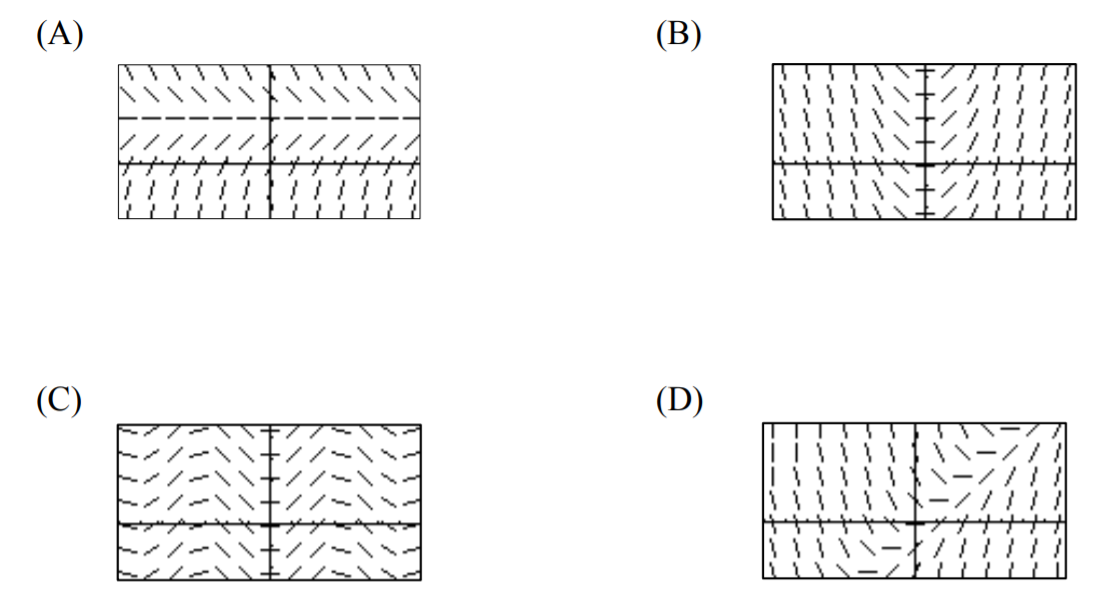
\includegraphics[width=\linewidth]{images/1.2-1.png}
\end{image}%
%
\begin{enumerate}[label=(\alph*)]
\item{}\(\frac{dy}{dt}=\sin t\)%
\item{}\(\frac{dy}{dt}=t-y\)%
\item{}\(\frac{dy}{dt}=2-y\)%
\item{}\(\frac{dy}{dt}=t\)%
\end{enumerate}
\end{divisionexercise}%
\begin{divisionexercise}{2}{}{}{g:exercise:idm45282412990864}%
Suppose the following ODE%
\begin{equation*}
\frac{dy}{dt}=y^{2}-t
\end{equation*}
has the following slope field: \begin{image}{0}{1}{0}%
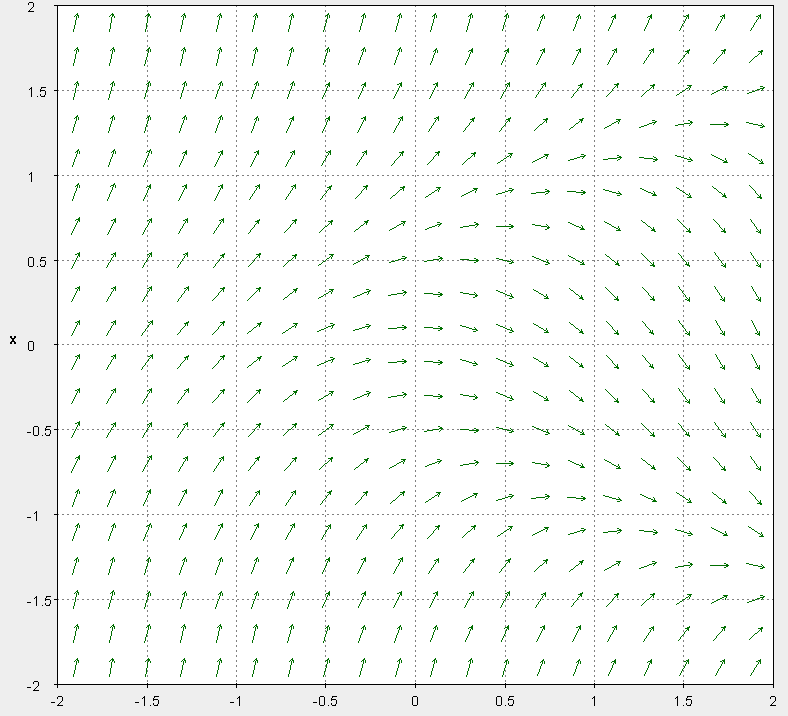
\includegraphics[width=\linewidth]{images/1.2-2.png}
\end{image}%
%
\begin{enumerate}[label=(\alph*)]
\item{}Suppose \(y(t)\) is a solution to this ODE and also you know that \(y\left(-1\right)=1\). Then based on the slope field, what is your prediction for the long term behavior of \(y(t)\). That is, what is your prediction of%
\begin{equation*}
\lim_{t\to\infty}y(t)?
\end{equation*}
%
\item{}Suppose \(y(t)\) is a solution to this ODE and also you know that \(y\left(1\right)=0\). Then based on the slope field, what is your prediction for the long term behavior of \(y(t)\), that is, what is your prediction of%
\begin{equation*}
\lim_{t\to\infty}y(t)=?
\end{equation*}
%
\end{enumerate}
\end{divisionexercise}%
\begin{divisionexercise}{3}{}{}{g:exercise:idm45282412984576}%
Let \(P(t)\) represent the population of the Phan fish breed. Suppose you come up with the following differential equation that models \(P(t)\):%
\begin{equation*}
\frac{dP}{dt}=P\left(P-100\right)\left(P+100\right)/100000
\end{equation*}
Its slope field is given by: \begin{image}{0}{1}{0}%
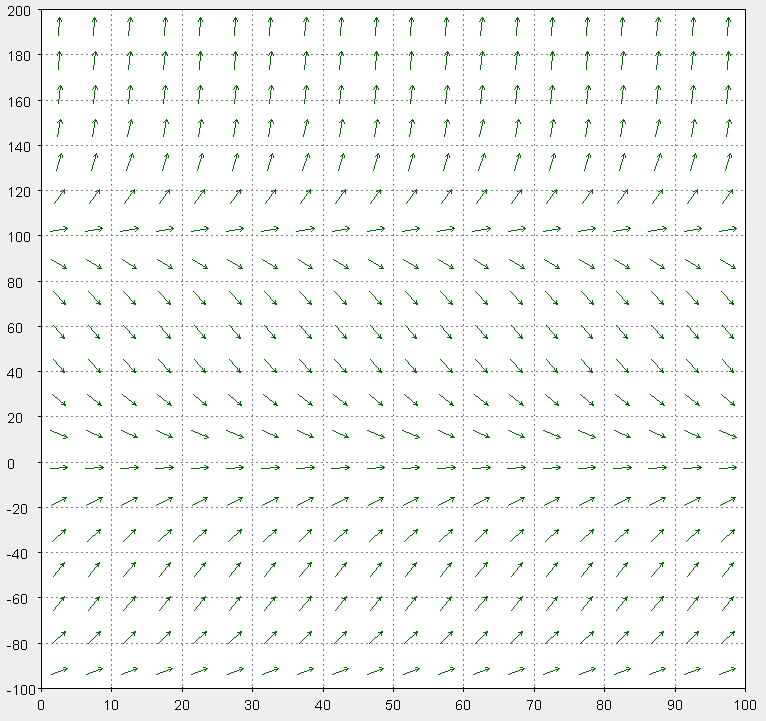
\includegraphics[width=\linewidth]{images/1.2-3b.png}
\end{image}%
%
\begin{enumerate}[label=(\alph*)]
\item{}Suppose that the population of the Phan fish is \(80\) at time \(t=0\). What is the long term behavior for the population of the Phan fish? Will it keep increasing\slash{}decreasing, stabilize to a certain number, or go extinct?%
\end{enumerate}
\end{divisionexercise}%
\end{exercises-subsection-numberless}
\end{sectionptx}
\end{appendixptx}
%
%
\typeout{************************************************}
\typeout{Appendix C Exercises for Chapter 2}
\typeout{************************************************}
%
\begin{appendixptx}{Exercises for Chapter 2}{}{Exercises for Chapter 2}{}{}{g:appendix:idm45282412860688}
%
%
\typeout{************************************************}
\typeout{Section C.1 Section~\ref*{x:section:ch2-1}}
\typeout{************************************************}
%
\begin{sectionptx}{Section~\ref*{x:section:ch2-1}}{}{Section~\ref*{x:section:ch2-1}}{}{}{g:section:idm45282412860112}
%
%
\typeout{************************************************}
\typeout{Exercises C.1 Exercises}
\typeout{************************************************}
%
\begin{exercises-subsection-numberless}{Exercises}{}{Exercises}{}{}{g:exercises:idm45282412859136}
\begin{divisionexercise}{1}{}{}{g:exercise:idm45282412858848}%
Use a computer app to draw the direction field for the given differential equations. Use the direction field to describe the long term behavior of the solution for large \(t\). (Meaning use the direction field to predict \(\lim_{t\to\infty}y(t)\) for different starting points). Find the general solution of the given differential equations, and use it to determine how solutions behave as \(t\to\infty\).%
%
\begin{enumerate}[label=(\alph*)]
\item{}\(y^{\prime}+3y=t+e^{-2t}\)%
\item{}\(y^{\prime}+y=te^{-t}+1\)%
\item{}\(ty^{\prime}-y=t^{2}e^{-t}\)%
\item{}\(2y^{\prime}+y=3t\)%
\end{enumerate}
\end{divisionexercise}%
\begin{divisionexercise}{2}{}{}{g:exercise:idm45282412852864}%
Find the particular solution to given initial value problem.%
%
\begin{enumerate}[label=(\alph*)]
\item{}\(y^{\prime}-y=2te^{2t}\), \(y(0)=1\)%
\item{}\(ty^{\prime}+2y=\sin t\), \(y\left(\pi/2\right)=1\), \(t>0\)%
\end{enumerate}
\end{divisionexercise}%
\begin{divisionexercise}{3}{}{}{g:exercise:idm45282412848656}%
Consider the following initial value problem:%
\begin{equation*}
ty^{\prime}+\left(t+1\right)y=2te^{-t},\,\,\,\,\,y(1)=a,\,\,\,\,t>0
\end{equation*}
where \(a\) is any real number. Find the particular solution that solves this IVP.%
\end{divisionexercise}%
\end{exercises-subsection-numberless}
\end{sectionptx}
%
%
\typeout{************************************************}
\typeout{Section C.2 Section~\ref*{x:section:ch2-2}}
\typeout{************************************************}
%
\begin{sectionptx}{Section~\ref*{x:section:ch2-2}}{}{Section~\ref*{x:section:ch2-2}}{}{}{g:section:idm45282412846400}
%
%
\typeout{************************************************}
\typeout{Exercises C.2 Exercises}
\typeout{************************************************}
%
\begin{exercises-subsection-numberless}{Exercises}{}{Exercises}{}{}{g:exercises:idm45282412845424}
\begin{divisionexercise}{1}{}{}{g:exercise:idm45282412845136}%
Find the general solutions for the following differential equations. Find the \emph{explicit} solutions if you can. If you can't solve for \(y\) exactly, then leave it as an \textbackslash{}emph\textbraceleft{}implicit\textbraceright{} solution:%
\begin{enumerate}[label=(\alph*)]
\item{}\(y^{\prime}=ky\) where \(k\) is a parameter.%
\item{}\({\displaystyle y^{\prime}=\frac{x^{2}}{y}}\)%
\item{}\({\displaystyle \frac{dy}{dx}=\frac{3x^{2}-1}{3+2y}}\)%
\item{}\(xy^{\prime}=\frac{\left(1-y^{2}\right)^{1/2}}{y}\)%
\item{}\({\displaystyle \frac{dy}{dx}=\frac{x^{2}}{1+y^{2}}}\)%
\item{}\({\displaystyle \frac{dy}{dx}=\frac{x}{\cos\left(y^{2}\right)y}}\)%
\end{enumerate}
%
\end{divisionexercise}%
\begin{divisionexercise}{2}{}{}{g:exercise:idm45282412970704}%
Consider the ODE%
\begin{equation*}
\frac{dy}{dt}=\frac{4y}{t}.
\end{equation*}
%
%
\begin{enumerate}[label=(\alph*)]
\item{}What kind of differential equation is this? Is it linear? Is it separable?%
\item{}If the ODE is both separable and Linear. Then use both methods to solve this equation. And check to make sure you get the same answer.%
\end{enumerate}
\end{divisionexercise}%
\begin{divisionexercise}{3}{}{}{g:exercise:idm45282412967712}%
Find the general solution to the following differential equation:%
\begin{equation*}
\frac{dy}{dt}=\left(y+1\right)\left(y-2\right).
\end{equation*}
(Hint: Use partial fractions!)%
\end{divisionexercise}%
\end{exercises-subsection-numberless}
\end{sectionptx}
%
%
\typeout{************************************************}
\typeout{Section C.3 Section~\ref*{x:section:ch2-3}}
\typeout{************************************************}
%
\begin{sectionptx}{Section~\ref*{x:section:ch2-3}}{}{Section~\ref*{x:section:ch2-3}}{}{}{g:section:idm45282412965936}
%
%
\typeout{************************************************}
\typeout{Exercises C.3 Exercises}
\typeout{************************************************}
%
\begin{exercises-subsection-numberless}{Exercises}{}{Exercises}{}{}{g:exercises:idm45282412964960}
\begin{divisionexercise}{1}{}{}{g:exercise:idm45282412964672}%
First check each if the following differential equations are homogeneous. Then find the general solutions for the following differential equations.%
\begin{enumerate}[label=(\alph*)]
\item{}\({\displaystyle x^{2}\frac{dy}{dx}=-\left(y^{2}-yx\right).}\)%
\item{}\({\displaystyle \frac{dy}{dx}=\frac{x+3y+2\frac{y^{2}}{x}}{3x+y}.}\)%
\item{}\({\displaystyle \frac{dy}{dx}=\frac{y}{x}-\frac{x^{2}-y^{2}}{2xy}.}\)%
\end{enumerate}
%
\end{divisionexercise}%
\begin{divisionexercise}{2}{}{}{g:exercise:idm45282412960992}%
Consider the following homogeneous equation:%
\begin{equation*}
\frac{dy}{dx}=\frac{y-x}{y+x}.
\end{equation*}
%
\begin{enumerate}[label=(\alph*)]
\item{}Use the substitution \(v=\frac{y}{x}\) to rewrite the equation only in terms of \(v\) and \(x\).%
\item{}Solve for the general solution.%
\end{enumerate}
%
\end{divisionexercise}%
\begin{divisionexercise}{3}{}{}{g:exercise:idm45282412956848}%
Consider the following homogeneous equation:%
\begin{equation*}
\frac{dy}{dx}=\frac{-y^{2}-yx}{x^{2}}.
\end{equation*}
%
\begin{enumerate}[label=(\alph*)]
\item{}Use the substitution \(v=\frac{y}{x}\) to rewrite the equation only in terms of \(v\) and \(x\).%
\item{}Solve for the general solution.%
\end{enumerate}
\end{divisionexercise}%
\begin{divisionexercise}{4}{}{}{g:exercise:idm45282412953152}%
Using the given substitution, solve the differential equation:%
%
\begin{enumerate}[label=(\alph*)]
\item{}Rewrite \({\displaystyle \frac{dy}{dx}+xy=x^{2}y^{2}}\) using the substitution \(u=\frac{1}{y}\), only in terms of \(u,x\).%
\item{}Rewrite \({\displaystyle \frac{dy}{dx}+y=\frac{x}{y^{2}}}\) using the substitution \(u=y^{3}\), only in terms of \(u,x\).%
\end{enumerate}
\end{divisionexercise}%
\end{exercises-subsection-numberless}
\end{sectionptx}
%
%
\typeout{************************************************}
\typeout{Section C.4 Section~\ref*{x:section:ch2-4}}
\typeout{************************************************}
%
\begin{sectionptx}{Section~\ref*{x:section:ch2-4}}{}{Section~\ref*{x:section:ch2-4}}{}{}{g:section:idm45282412947760}
%
%
\typeout{************************************************}
\typeout{Exercises C.4 Exercises}
\typeout{************************************************}
%
\begin{exercises-subsection-numberless}{Exercises}{}{Exercises}{}{}{g:exercises:idm45282412946944}
\begin{divisionexercise}{1}{}{}{g:exercise:idm45282412946656}%
Initially, a tank contains 100 L of water with 10 kg of sugar in solution. Water containing sugar flows into the tank at the rate of \(2\) L\slash{}min, and the well-stirred mixture in the tank flows out at the rate of \(5\) L\slash{}min. The concentration \(c(t)\) of sugar in the incoming water varies as \(c(t)=2+\cos(3t)\) kg\slash{}L. Let \(Q(t)\) be the amount of sugar (in kilograms) in the tank at time \(t\) (in minutes). Write the Initial Value Problem that \(Q(t)\) satisfies.%
\end{divisionexercise}%
\begin{divisionexercise}{2}{}{}{g:exercise:idm45282411768176}%
Initially, a tank contains \(500\) L (liters) of pure water. Water containing \(0.3\)kg of salt per liter is entering at a rate of \(2\) L\slash{}min, and the mixture is allowed to flow out of the tank at a rate of \(1\) L\slash{}min. Let \(Q(t)\) be the amount of salt at time \(t\) measured in kilograms (kg). What is the IVP that \(Q(t)\) satisfies?%
\end{divisionexercise}%
\begin{divisionexercise}{3}{}{}{g:exercise:idm45282411763936}%
Initially, a tank contains \(400\) L of water with \(10\) kg of salt in solution. Water containing \(0.1\) kg of salt per liter (L) is entering at a rate of \(1\) L\slash{}min, and the mixture is allowed to flow out of the tank at a rate of \(2\) L\slash{}min. Let \(Q(t)\) be the amount of salt at time \(t\) measured in kilograms. What is the IVP that \(Q(t)\) satisfies?%
\end{divisionexercise}%
\begin{divisionexercise}{4}{}{}{g:exercise:idm45282411759248}%
Consider a pond that initially constains \(10\) million gal of pure water. Water containing a polluted chemical flows into the pond at the rate of \(6\) million gal\slash{}year, and the mixture in the pond flows out at the rate of \(5\) million gal\slash{}year. The concentration \(\gamma(t)\) of chemical in the incoming water varies as \(\gamma(t)=2+\sin2t\) grams\slash{}gal. Let \(Q(t)\) be the amount of chemical at time \(t\) measured by millions of grams. What is the IVP that \(Q(t)\) satisfies?%
\end{divisionexercise}%
\begin{divisionexercise}{5}{}{}{g:exercise:idm45282411754464}%
A tank contains \(200\) gal of liquid. Initially, the tank contains pure water. At time \(t=0\), brine containing \(3\) lb\slash{}gal of salt begins to pour into the tank at a rate of \(2\) gal\slash{}min, and the well-stirred mixture is allowed to drain away at the same rate. How many minutes must elapse before there are \(100\) lb of salt in the tank?%
\end{divisionexercise}%
\begin{divisionexercise}{6}{}{}{g:exercise:idm45282411751088}%
A huge tank initially contains \(10\) gallons (gal) of water with \(6\) lb of salt in solution. Water containing \(1\) lb of salt per gallon is entering at a rate of \(3\) gal\slash{}min, and the well-stirred mixture is allowed to flow out of the tank at a rate of \(2\) gal\slash{}min. What is the amount of the salt in the tank after \(10\) min?%
\end{divisionexercise}%
\begin{divisionexercise}{7}{}{}{g:exercise:idm45282411747280}%
Initially a tank holds \(40\) gallons of water with \(10\) lb of salt in solution. A salt solution containing \(\frac{1}{2}\)b of salt per gallon runs into the tank at the rate of \(4\) gallons per minute. The well mixed solution runs out of the tank at a rate of 2 gallons per minute. Let \(y(t)\) be the amount of salt in the tank after \(t\) minutes. Then what is \(y(20)\).%
\end{divisionexercise}%
\end{exercises-subsection-numberless}
\end{sectionptx}
%
%
\typeout{************************************************}
\typeout{Section C.5 Section~\ref*{x:section:ch2-5}}
\typeout{************************************************}
%
\begin{sectionptx}{Section~\ref*{x:section:ch2-5}}{}{Section~\ref*{x:section:ch2-5}}{}{}{g:section:idm45282411742672}
%
%
\typeout{************************************************}
\typeout{Exercises C.5 Exercises}
\typeout{************************************************}
%
\begin{exercises-subsection-numberless}{Exercises}{}{Exercises}{}{}{g:exercises:idm45282411741696}
\begin{divisionexercise}{1}{}{}{g:exercise:idm45282411741408}%
A detective is called to the scene of a crime where a dead body has just been found.%
\begin{enumerate}[label=(\alph*)]
\item{}She arrives on the scene at 10:23 pm and begins her investigation. Immediately, the temperature of the body is taken and is found to be \(80^{\circ}\)F. The detective checks the programmable thermostat and finds that the room has been kept at a constant \(68^{\circ}\)F for the past 3 days.%
 \textbackslash{}\item{}After evidence from the crime scene is collected, the temperature of the body is taken once more and found to be \(78.5^{\circ}\) F. This last temperature reading was taken exactly one hour after the first one.%
\item{}The next day the detective is asked by another investigator, ``What time did our victim die?'' Assuming that the victim's body temperature was normal (\(98.6^{\circ}\)) prior to death, what is her answer to this question? Newton's Law of Cooling can be used to determine a victim's time of death.%
\end{enumerate}
%
\end{divisionexercise}%
\end{exercises-subsection-numberless}
\end{sectionptx}
%
%
\typeout{************************************************}
\typeout{Section C.6 Section~\ref*{x:section:ch2-6}}
\typeout{************************************************}
%
\begin{sectionptx}{Section~\ref*{x:section:ch2-6}}{}{Section~\ref*{x:section:ch2-6}}{}{}{g:section:idm45282411735584}
%
%
\typeout{************************************************}
\typeout{Exercises C.6 Exercises}
\typeout{************************************************}
%
\begin{exercises-subsection-numberless}{Exercises}{}{Exercises}{}{}{g:exercises:idm45282411734608}
\begin{divisionexercise}{1}{}{}{g:exercise:idm45282411734320}%
What is the largest open interval in which the solution to the IVPs in part (a) and part (b) are guaranteed to exist by the existence and uniqueness theorems?%
\begin{enumerate}[label=(\alph*)]
\item{}The IVP given by:%
\begin{equation*}
\begin{cases}
\left(t^{2}+t-2\right)y^{\prime}+e^{t}y=\frac{\left(t-4\right)}{\left(t-6\right)}\\
y(-3)=-1.
\end{cases}
\end{equation*}
%
\item{}The IVP given by:%
\begin{equation*}
\begin{cases}
\left(t^{2}+t-2\right)y^{\prime}+e^{t}y=\frac{\left(t-4\right)}{\left(t-6\right)}\\
y(5)=47.
\end{cases}
\end{equation*}
%
\end{enumerate}
%
\end{divisionexercise}%
\begin{divisionexercise}{2}{}{}{g:exercise:idm45282411731056}%
What is the largest open interval in which the solution of the initial value problem%
\begin{equation*}
\begin{cases}
\left(t-3\right)y^{\prime}+y=\frac{\left(t-3\right)\cdot\ln\left(t-1\right)}{t-10}\\
y(6)=-7.
\end{cases}
\end{equation*}
is guaranteed to exist by the existence and uniqueness Theorem?%
\end{divisionexercise}%
\begin{divisionexercise}{3}{}{}{g:exercise:idm45282411729456}%
What is the largest open interval in which the solution of the initial value problem%
\begin{equation*}
\begin{cases}
\left(t-1\right)y^{\prime}+\sqrt{t+2}y=\frac{3}{t-3}\\
y(2)=-5.
\end{cases}
\end{equation*}
is guaranteed to exist by the Existence and Uniqueness Theorem?%
\end{divisionexercise}%
\begin{divisionexercise}{4}{}{}{g:exercise:idm45282411727872}%
What is the largest open interval in which the solution of the initial value problem%
\begin{equation*}
\begin{cases}
t^{2}y^{\prime}+\ln\left|t-4\right|y=\frac{t-1}{\sin t}\\
y(5)=9.
\end{cases}
\end{equation*}
is guaranteed to exist by the existence and uniqueness Theorem?%
\end{divisionexercise}%
\begin{divisionexercise}{5}{}{}{g:exercise:idm45282411726288}%
Consider the IVP below%
\begin{equation*}
\frac{dy}{dt}=y^{1/5},\,\,\,\,y(0)=0.
\end{equation*}
%
%
\begin{enumerate}[label=(\alph*)]
\item{}Is this a linear or nonlinear equation? Can you use \hyperref[x:theorem:existencethm1]{Theorem~\ref{x:theorem:existencethm1}}?%
\item{}Using \hyperref[x:theorem:existencethm2]{Theorem~\ref{x:theorem:existencethm2}} (the general theorem), can you guarantee that there is a unique solution to this IVP? Why?%
\end{enumerate}
\end{divisionexercise}%
\end{exercises-subsection-numberless}
\end{sectionptx}
%
%
\typeout{************************************************}
\typeout{Section C.7 Section~\ref*{x:section:ch2-7}}
\typeout{************************************************}
%
\begin{sectionptx}{Section~\ref*{x:section:ch2-7}}{}{Section~\ref*{x:section:ch2-7}}{}{}{g:section:idm45282411722160}
%
%
\typeout{************************************************}
\typeout{Exercises C.7 Exercises}
\typeout{************************************************}
%
\begin{exercises-subsection-numberless}{Exercises}{}{Exercises}{}{}{g:exercises:idm45282411721344}
\begin{divisionexercise}{1}{}{}{g:exercise:idm45282411721056}%
Consider the following differential equation:%
\begin{equation*}
\frac{dy}{dt}=\left(y+2\right)\left(y-1\right)\left(y+5\right)
\end{equation*}
%
%
\begin{enumerate}[label=(\alph*)]
\item{}Draw a phase line. Classify the equilibrium solutions. \textbackslash{}item Draw all possible sketch of solutions of this differential equation.%
\item{}Consider the IVP%
\begin{equation*}
\frac{dy}{dt}=\left(y+2\right)\left(y-1\right)\left(y+5\right),\,\,\,\,\,\,y(0)=3.
\end{equation*}
Let \(y(t)\) be the unique solution that solves this IVP. Draw a sketch of \(y(t)\) and use it to find \(\lim_{t\to\infty}y(t)\) and \(\lim_{t\to-\infty}y(t)\)?%
\end{enumerate}
\end{divisionexercise}%
\begin{divisionexercise}{2}{}{}{g:exercise:idm45282411715936}%
Consider the following differential equation:%
\begin{equation*}
\frac{dy}{dt}=y\left(y-3\right)^{2}\left(y+4\right)
\end{equation*}
%
%
\begin{enumerate}[label=(\alph*)]
\item{}Draw a phase line. Classify the equilibrium solutions.%
\item{}Draw all possible sketch of solutions of this differential equation.%
\item{}Consider the IVP%
\begin{equation*}
\frac{dy}{dt}=y\left(y-3\right)^{2}\left(y+4\right),\,\,\,\,\,\,y(0)=-5.
\end{equation*}
Let \(y(t)\) be the unique solution that solves this IVP. Draw a sketch of \(y(t)\) and use it to find \(\lim_{t\to\infty}y(t)\) and \(\lim_{t\to-\infty}y(t)\)?%
\item{}Consider the IVP%
\begin{equation*}
\frac{dy}{dt}=y\left(y-3\right)^{2}\left(y+4\right),\,\,\,\,\,\,y(0)=1.
\end{equation*}
Let \(y(t)\) be the unique solution that solves this IVP. Draw a sketch of \(y(t)\) and use it to find \(\lim_{t\to\infty}y(t)\) and \(\lim_{t\to-\infty}y(t)\)?%
\end{enumerate}
\end{divisionexercise}%
\begin{divisionexercise}{3}{}{}{g:exercise:idm45282411707808}%
Let \(y(t)\) be the unique solution to the IVP given by%
\begin{equation*}
\frac{dy}{dt}=y^{2}\sin y,\,\,\,\,\,\,y(0)=1.
\end{equation*}
Draw a phase line for the ODE to find out \(\lim_{t\to\infty}y(t)\) for the unique solution of the IVP above.%
\end{divisionexercise}%
\begin{divisionexercise}{4}{}{}{g:exercise:idm45282411705424}%
Consider the differential equation%
\begin{equation*}
\frac{dy}{dt}=f\left(y\right)
\end{equation*}
where \(f(y)\) is given by the following graph (in \(y\) versus \(f(y)\)):%
\begin{image}{0}{1}{0}%
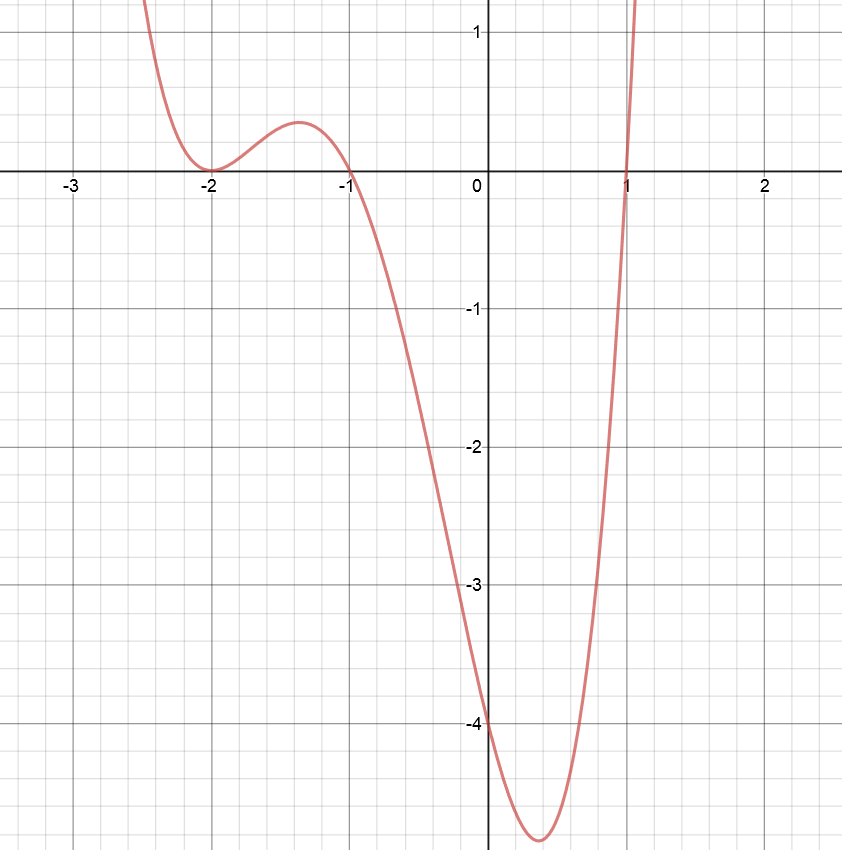
\includegraphics[width=\linewidth]{images/2.7-4.png}
\end{image}%
Draw the phase line and classify the equilibrium solutions.%
\end{divisionexercise}%
\end{exercises-subsection-numberless}
\end{sectionptx}
%
%
\typeout{************************************************}
\typeout{Section C.8 Section~\ref*{x:section:ch2-8}}
\typeout{************************************************}
%
\begin{sectionptx}{Section~\ref*{x:section:ch2-8}}{}{Section~\ref*{x:section:ch2-8}}{}{}{g:section:idm45282411701280}
%
%
\typeout{************************************************}
\typeout{Exercises C.8 Exercises}
\typeout{************************************************}
%
\begin{exercises-subsection-numberless}{Exercises}{}{Exercises}{}{}{g:exercises:idm45282411700464}
\begin{divisionexercise}{1}{}{}{g:exercise:idm45282411700176}%
Determine whether each of the following equations are exact. If it is exact, find the solution. Implicit solutions are fine. %
\begin{enumerate}[label=(\alph*)]
\item{}\({\displaystyle \left(2x+3\right)+\left(2y-2\right)y^{\prime}=0}\)%
\item{}\({\displaystyle \left(2x+4y\right)+\left(2x-2y\right)y^{\prime}=0}\)%
\item{}\(\left(3x^{2}-2xy+2\right)dx+\left(6y^{2}-x^{2}+3\right)dy=0\)%
\item{}\({\displaystyle \left(2xy^{2}+2y\right)+\left(2x^{2}y+2x\right)y^{\prime}=0}\)%
\item{}\({\displaystyle \frac{dy}{dx}=-\frac{ax+by}{bx+cy}}\)%
\item{}\({\displaystyle \left(e^{x}\sin y+3y\right)dx-\left(3x-e^{x}\sin y\right)dy=0}\)%
\item{}\({\displaystyle \left(\frac{y}{x}+6x\right)dx+\left(\ln x-2\right)dy=0},\)\(x>0\)%
\end{enumerate}
\end{divisionexercise}%
\begin{divisionexercise}{2}{}{}{g:exercise:idm45282411693520}%
Find the implicit particular solution to the initial value problem%
\begin{equation*}
\left(9x^{2}+y-1\right)dx-\left(4y-x\right)dy=0,\,\,\,\,\,\,y(1)=0.
\end{equation*}
\end{divisionexercise}%
\begin{divisionexercise}{3}{}{}{g:exercise:idm45282411692496}%
Find the values of \(b\) for which the given equation is exact.%
\begin{equation*}
\left(ye^{2xy}+x\right)dx+bxe^{2xy}dy=0.
\end{equation*}
\end{divisionexercise}%
\end{exercises-subsection-numberless}
\end{sectionptx}
%
%
\typeout{************************************************}
\typeout{Section C.9 Section~\ref*{x:section:ch2-9}}
\typeout{************************************************}
%
\begin{sectionptx}{Section~\ref*{x:section:ch2-9}}{}{Section~\ref*{x:section:ch2-9}}{}{}{g:section:idm45282411690768}
%
%
\typeout{************************************************}
\typeout{Exercises C.9 Exercises}
\typeout{************************************************}
%
\begin{exercises-subsection-numberless}{Exercises}{}{Exercises}{}{}{g:exercises:idm45282411689952}
\begin{divisionexercise}{1}{}{}{g:exercise:idm45282411689664}%
Find the approximate values of the solution of the given initial value problem at \(t=0.1,0.2,0.3\) and \(0.4\) using Euler's Method with \(h=0.1\).%
\begin{equation*}
\frac{dy}{dt}=t+y,\,\,\,\,\,y(0)=1.
\end{equation*}
%
\end{divisionexercise}%
\begin{divisionexercise}{2}{}{}{g:exercise:idm45282411687008}%
Find the approximate values of the solution of the given initial value problem at \(t=0.1,0.2,0.3\) and \(0.4\) using Euler's Method with \(h=0.05\).%
\begin{equation*}
\frac{dy}{dt}=t+y^{2},\,\,\,\,\,y(0)=1.
\end{equation*}
%
\end{divisionexercise}%
\begin{divisionexercise}{3}{}{}{g:exercise:idm45282411684336}%
Find the approximate value of \(y\left(2\right)\) using Euler's Method with \(h=0.5\) for the solution of the following IVP%
\begin{equation*}
\frac{dy}{dt}=y\left(3-ty\right),\,\,\,\,\,y(0)=0.5.
\end{equation*}
%
\end{divisionexercise}%
\begin{divisionexercise}{4}{}{}{g:exercise:idm45282411682144}%
Consider the solution \(y(t)\) to the IVP:%
\begin{equation*}
\frac{dy}{dt}=y\left(t+y\right)/10,\,\,\,\,\,y(0)=1.
\end{equation*}
Use the slope field below with Euler's Method (using \(h=.5\)) to estimate the value of \(y(3)\): \begin{image}{0}{1}{0}%
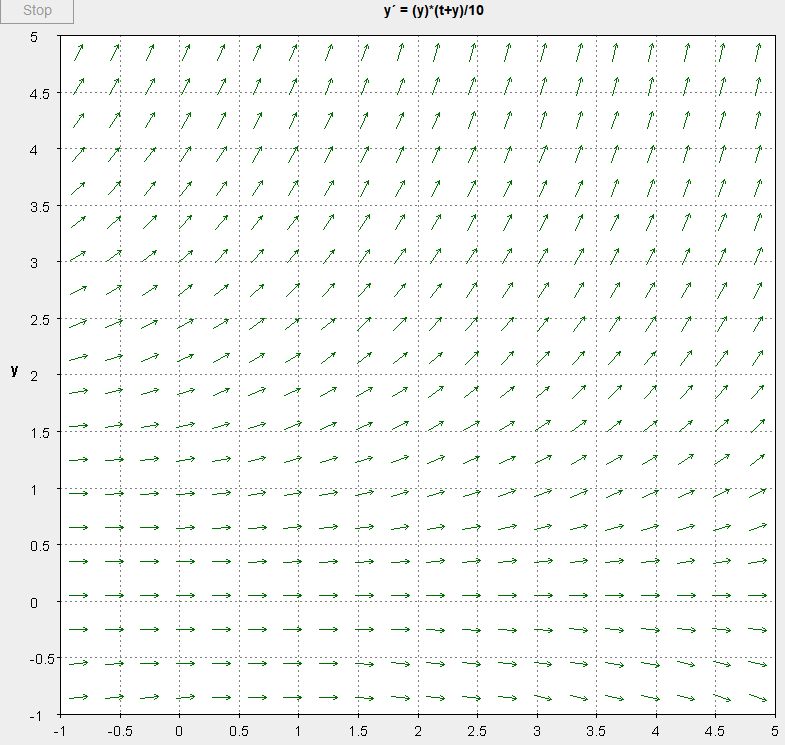
\includegraphics[width=\linewidth]{images/2.9-4.png}
\end{image}%
%
\end{divisionexercise}%
\end{exercises-subsection-numberless}
\end{sectionptx}
\end{appendixptx}
%
%
\typeout{************************************************}
\typeout{Appendix D Exercises for Chapter 3}
\typeout{************************************************}
%
\begin{appendixptx}{Exercises for Chapter 3}{}{Exercises for Chapter 3}{}{}{g:appendix:idm45282411678464}
%
%
\typeout{************************************************}
\typeout{Section D.1 Section~\ref*{x:section:ch3-2}}
\typeout{************************************************}
%
\begin{sectionptx}{Section~\ref*{x:section:ch3-2}}{}{Section~\ref*{x:section:ch3-2}}{}{}{g:section:idm45282411677888}
%
%
\typeout{************************************************}
\typeout{Exercises D.1 Exercises}
\typeout{************************************************}
%
\begin{exercises-subsection-numberless}{Exercises}{}{Exercises}{}{}{g:exercises:idm45282411677072}
\begin{divisionexercise}{1}{}{}{g:exercise:idm45282411676784}%
Check if the following function are solutions to the given EQ.%
\begin{enumerate}[label=(\alph*)]
\item{}Check directly if \(y_{1}=2e^{5t}\) is a solution or not to \(y^{\prime\prime}-6y^{\prime}+5y=0\).%
\item{}Check directly if \(y_{2}=2e^{t}\) is a solution or not to \(y^{\prime\prime}-6y^{\prime}+5y=t\).%
\end{enumerate}
%
\end{divisionexercise}%
\begin{divisionexercise}{2}{}{}{g:exercise:idm45282411672800}%
Recall that if \(y(t)=e^{rt}\) is a solution to the ODE given by%
\begin{equation*}
ay^{\prime\prime}+by^{\prime}+cy=0
\end{equation*}
for constant \(a,b,c\) where \(a\ne0\), then the exponent \(r\) in front the \(t\) must be a solution to the \emph{characteristic equation} \(ar^{2}+br+c=0\).%
\par
By yourself, rederive that if \(y(t)=Ae^{rt}\) is a solution to the equation above, then the number \(r\) must satisfy the characteristic equation \(ar^{2}+br+c=0\) or \(A=0\).%
\end{divisionexercise}%
\begin{divisionexercise}{3}{}{}{g:exercise:idm45282411665904}%
Use the method given in Section 3.1 to find the general solution to%
\begin{equation*}
y^{\prime\prime}+5y^{\prime}-6y=0
\end{equation*}
%
\end{divisionexercise}%
\begin{divisionexercise}{4}{}{}{g:exercise:idm45282411664624}%
Use the method given in Section 3.1 to find the general solution to%
\begin{equation*}
y^{\prime\prime}-7y^{\prime}=0
\end{equation*}
%
\end{divisionexercise}%
\begin{divisionexercise}{5}{}{}{g:exercise:idm45282411663344}%
Use the method given in Section 3.1 to find the particular solution to the IVP%
\begin{equation*}
y^{\prime\prime}+y^{\prime}-20y=0,\,\,\,\,\,y(0)=18,y^{\prime}(0)=9
\end{equation*}
%
\end{divisionexercise}%
\end{exercises-subsection-numberless}
\end{sectionptx}
%
%
\typeout{************************************************}
\typeout{Section D.2 Section~\ref*{x:section:ch3-3}}
\typeout{************************************************}
%
\begin{sectionptx}{Section~\ref*{x:section:ch3-3}}{}{Section~\ref*{x:section:ch3-3}}{}{}{g:section:idm45282411661696}
%
%
\typeout{************************************************}
\typeout{Exercises D.2 Exercises}
\typeout{************************************************}
%
\begin{exercises-subsection-numberless}{Exercises}{}{Exercises}{}{}{g:exercises:idm45282411660880}
\begin{divisionexercise}{1}{}{}{g:exercise:idm45282411660592}%
What is the largest open interval in which the solution of the initial value problem%
\begin{equation*}
\left(t-3\right)y^{\prime\prime}+\sin ty^{\prime}+y=\frac{\ln\left(t-1\right)}{t-10}, \hspace{.2in}
y(15)=-7,y^{\prime}(15)=10
\end{equation*}
is guaranteed to exist by \hyperref[x:theorem:thm2ndexist]{Theorem~\ref{x:theorem:thm2ndexist}}?%
\end{divisionexercise}%
\begin{divisionexercise}{2}{}{}{g:exercise:idm45282411658464}%
What is the largest open interval in which the solution of the initial value problem%
\begin{equation*}
t^{2}y^{\prime\prime}+e^{t}y^{\prime}+\left(t-1\right)y=\sqrt{t+2}, \hspace{.1in}
y(-1)=1,y^{\prime}(-1)=5
\end{equation*}
is guaranteed to exist by \hyperref[x:theorem:thm2ndexist]{Theorem~\ref{x:theorem:thm2ndexist}}?%
\end{divisionexercise}%
\begin{divisionexercise}{3}{}{}{g:exercise:idm45282411656352}%
Consider the equation%
\begin{equation*}
y^{\prime\prime}+p(t)y^{\prime}+q(t)y=0,
\end{equation*}
where \(p,q\) are continuous in some interval \(I\). What are the two things you have to do by \hyperref[x:theorem:thmgensol]{Theorem~\ref{x:theorem:thmgensol}} in order to find the general solution to the ODE above?\end{divisionexercise}%
\begin{divisionexercise}{4}{}{}{g:exercise:idm45282411653856}%
Consider the equation%
\begin{equation*}
2t^{2}y^{\prime\prime}+3ty^{\prime}-y=0,\,\,\,\,\,t>0.
\end{equation*}
%
%
\begin{enumerate}[label=(\alph*)]
\item{}Is the function \(y_{1}(t)=t^{\frac{1}{2}}\) a solution to this ODE?%
\item{}Is the function \(y_{2}(t)=t^{-1}\) a solution to this ODE?%
\item{}Use \hyperref[x:theorem:thmgensol]{Theorem~\ref{x:theorem:thmgensol}} to show that%
\begin{equation*}
y(t)=c_{1}t^{\frac{1}{2}}+c_{2}t^{-1}
\end{equation*}
gives the general solution to the ODE above.%
\end{enumerate}
\end{divisionexercise}%
\end{exercises-subsection-numberless}
\end{sectionptx}
%
%
\typeout{************************************************}
\typeout{Section D.3 Section~\ref*{x:section:ch3-4}}
\typeout{************************************************}
%
\begin{sectionptx}{Section~\ref*{x:section:ch3-4}}{}{Section~\ref*{x:section:ch3-4}}{}{}{g:section:idm45282411648480}
%
%
\typeout{************************************************}
\typeout{Exercises D.3 Exercises}
\typeout{************************************************}
%
\begin{exercises-subsection-numberless}{Exercises}{}{Exercises}{}{}{g:exercises:idm45282411647504}
\begin{divisionexercise}{1}{}{}{g:exercise:idm45282411647216}%
Find the general solution of the following second order linear ODEs with constant coefficients. %
\begin{enumerate}[label=(\alph*)]
\item{}\({\displaystyle y^{\prime\prime}+16y=0}\)%
\item{}\(y^{\prime\prime}-4y^{\prime}+9y=0\)%
\item{}\(y^{\prime\prime}-4y^{\prime}+29y=0\)%
\end{enumerate}
\end{divisionexercise}%
\begin{divisionexercise}{2}{}{}{g:exercise:idm45282411644448}%
Find the particular solution to the following IVP:%
\begin{equation*}
{\displaystyle y^{\prime\prime}-8y^{\prime}+17y=0},\,\,\,\,\,\,y(0)=-4,y^{\prime}(0)=-1.
\end{equation*}
\end{divisionexercise}%
\end{exercises-subsection-numberless}
\end{sectionptx}
%
%
\typeout{************************************************}
\typeout{Section D.4 Section~\ref*{x:section:ch3-5}}
\typeout{************************************************}
%
\begin{sectionptx}{Section~\ref*{x:section:ch3-5}}{}{Section~\ref*{x:section:ch3-5}}{}{}{g:section:idm45282411643104}
%
%
\typeout{************************************************}
\typeout{Subsection D.4.1 Repeated roots}
\typeout{************************************************}
%
\begin{subsectionptx}{Repeated roots}{}{Repeated roots}{}{}{g:subsection:idm45282411642128}
%
%
\typeout{************************************************}
\typeout{Exercises D.4.1 Exercises}
\typeout{************************************************}
%
\begin{exercises-subsubsection-numberless}{Exercises}{}{Exercises}{}{}{g:exercises:idm45282411641392}
\begin{divisionexercise}{1}{}{}{g:exercise:idm45282411641104}%
Find the general solution of the following 2nd Order Linear ODEs with constant coefficients. %
\begin{enumerate}[label=(\alph*)]
\item{}\({\displaystyle y^{\prime\prime}+14y^{\prime}+49y=0}\)%
\item{}\(y^{\prime\prime}-18y^{\prime}+81y=0\)%
\end{enumerate}
\end{divisionexercise}%
\begin{divisionexercise}{2}{}{}{g:exercise:idm45282411638576}%
Find the particular solution to the following IVP:%
\begin{equation*}
{\displaystyle y^{\prime\prime}-4y^{\prime}+4y=0},\,\,\,\,\,\,y(0)=12,y^{\prime}(0)=-3.
\end{equation*}
\end{divisionexercise}%
\end{exercises-subsubsection-numberless}
\end{subsectionptx}
%
%
\typeout{************************************************}
\typeout{Subsection D.4.2 Reduction of order}
\typeout{************************************************}
%
\begin{subsectionptx}{Reduction of order}{}{Reduction of order}{}{}{g:subsection:idm45282411637200}
%
%
\typeout{************************************************}
\typeout{Exercises D.4.2 Exercises}
\typeout{************************************************}
%
\begin{exercises-subsubsection-numberless}{Exercises}{}{Exercises}{}{}{g:exercises:idm45282411636464}
\begin{divisionexercise}{1}{}{}{g:exercise:idm45282411636176}%
Suppose you know that \(y_{1}(t)=t\) is a solution to%
\begin{equation*}
t^{2}y^{\prime\prime}-3ty^{\prime}+3y=0,\,\,\,\,\,t>0.
\end{equation*}
Find a second solution \(y_{2}(t)\) that makes \(y=c_{1}y_{1}+c_{2}y_{2}\) the general solution of this ODE.\end{divisionexercise}%
\begin{divisionexercise}{2}{}{}{g:exercise:idm45282411633792}%
Suppose you know that \(y_{1}(t)=t^{-1}\) is a solution to%
\begin{equation*}
2t^{2}y^{\prime\prime}+ty^{\prime}-3y=0,\,\,\,\,\,t>0.
\end{equation*}
Find a second solution \(y_{2}(t)\) that makes \(y=c_{1}y_{1}+c_{2}y_{2}\) the general solution of this ODE.\end{divisionexercise}%
\begin{divisionexercise}{3}{}{}{g:exercise:idm45282411631408}%
Suppose you know that \(y_{1}(t)=t\) is a solution to%
\begin{equation*}
t^{2}y^{\prime\prime}+2ty^{\prime}-2y=0,\,\,\,\,\,t>0.
\end{equation*}
Find a second solution \(y_{2}(t)\) that makes \(y=c_{1}y_{1}+c_{2}y_{2}\) the general solution of this ODE.\end{divisionexercise}%
\begin{divisionexercise}{4}{}{}{g:exercise:idm45282411629024}%
Suppose you know that \(y_{1}(t)=t^{2}\) is a solution to%
\begin{equation*}
t^{2}y^{\prime\prime}-3ty^{\prime}+4y=0,\,\,\,\,\,t>0.
\end{equation*}
Find a second solution \(y_{2}(t)\) that makes \(y=c_{1}y_{1}+c_{2}y_{2}\) the general solution of this ODE.\end{divisionexercise}%
\end{exercises-subsubsection-numberless}
\end{subsectionptx}
\end{sectionptx}
%
%
\typeout{************************************************}
\typeout{Section D.5 Section~\ref*{x:section:ch3-6}}
\typeout{************************************************}
%
\begin{sectionptx}{Section~\ref*{x:section:ch3-6}}{}{Section~\ref*{x:section:ch3-6}}{}{}{g:section:idm45282411626160}
%
%
\typeout{************************************************}
\typeout{Exercises D.5 Exercises}
\typeout{************************************************}
%
\begin{exercises-subsection-numberless}{Exercises}{}{Exercises}{}{}{g:exercises:idm45282411625184}
\begin{divisionexercise}{1}{}{}{g:exercise:idm45282411624896}%
Consider the following non-homogeneous 2nd order ODE:%
\begin{equation*}
y^{\prime\prime}+y^{\prime}-2y=e^{3t}.
\end{equation*}
%
\begin{enumerate}[label=(\alph*)]
\item{}Find the general solution.%
\item{}Find the particular solution to the IVP:%
\begin{equation*}
y^{\prime\prime}+y^{\prime}-2y=e^{3t},\,\,\,\,y(0)=\frac{1}{10},y^{\prime}(0)=\frac{13}{10}.
\end{equation*}
%
\end{enumerate}
\end{divisionexercise}%
\begin{divisionexercise}{2}{}{}{g:exercise:idm45282411621984}%
Find the general solution to the following non-homogeneous 2nd order ODE:%
\begin{equation*}
y^{\prime\prime}-2y^{\prime}+2y=e^{2t}.
\end{equation*}
\end{divisionexercise}%
\begin{divisionexercise}{3}{}{}{g:exercise:idm45282411620976}%
Find the general solution to the following non-homogeneous 2nd order ODE:%
\begin{equation*}
y^{\prime\prime}-4y^{\prime}+3y=4e^{3t}.
\end{equation*}
%
\end{divisionexercise}%
\begin{divisionexercise}{4}{}{}{g:exercise:idm45282411619696}%
Find the general solution to the following non-homogeneous 2nd order ODE:%
\begin{equation*}
y^{\prime\prime}-2y^{\prime}+y=e^{t}.
\end{equation*}
%
\end{divisionexercise}%
\begin{divisionexercise}{5}{}{}{g:exercise:idm45282411618416}%
Find the general solution to the following non-homogeneous 2nd order ODE:%
\begin{equation*}
y^{\prime\prime}+y^{\prime}-6y=52\cos\left(2t\right).
\end{equation*}
%
\end{divisionexercise}%
\begin{divisionexercise}{6}{}{}{g:exercise:idm45282411617120}%
Find the general solution to the following non-homogeneous 2nd order ODE:%
\begin{equation*}
y^{\prime\prime}+2y^{\prime}+3y=\sin\left(t\right).
\end{equation*}
%
\end{divisionexercise}%
\begin{divisionexercise}{7}{}{}{g:exercise:idm45282411615824}%
For the following ODEs. Use the method of undertermined coefficients (MOUC) to make the correct guess for the \(y_{p}\). You DO NOT have to solve for the coefficients, \(A,B,C\dots\). Simply make the correct guess for the \(y_{p}\).%
\begin{enumerate}[label=(\alph*)]
\item{}\(y^{\prime\prime}-2y^{\prime}+y=te^{t},\)%
\item{}\(y^{\prime\prime}+y^{\prime}-2y=t^{2}e^{t},\)%
\item{}\(y^{\prime\prime}+y^{\prime}=t^{2}+\cos t,\)%
\item{}\(y^{\prime\prime}+y^{\prime}-6y=e^{5t}+\sin(3t),\)%
\item{}\(y^{\prime\prime}+y^{\prime}-2y=te^{t}+t^{2},\)%
\end{enumerate}
%
\end{divisionexercise}%
\end{exercises-subsection-numberless}
\end{sectionptx}
\end{appendixptx}
%
\backmatter
%
\end{document}